\PassOptionsToPackage{unicode=true}{hyperref} % options for packages loaded elsewhere
\PassOptionsToPackage{hyphens}{url}
\PassOptionsToPackage{dvipsnames,svgnames*,x11names*}{xcolor}
%
\documentclass[12pt,]{krantz}
\usepackage{lmodern}
\usepackage{amssymb,amsmath}
\usepackage{ifxetex,ifluatex}
\usepackage{fixltx2e} % provides \textsubscript
\ifnum 0\ifxetex 1\fi\ifluatex 1\fi=0 % if pdftex
  \usepackage[T1]{fontenc}
  \usepackage[utf8]{inputenc}
  \usepackage{textcomp} % provides euro and other symbols
\else % if luatex or xelatex
  \usepackage{unicode-math}
  \defaultfontfeatures{Ligatures=TeX,Scale=MatchLowercase}
    \setmonofont[Mapping=tex-ansi,Scale=0.7]{Source Code Pro}
\fi
% use upquote if available, for straight quotes in verbatim environments
\IfFileExists{upquote.sty}{\usepackage{upquote}}{}
% use microtype if available
\IfFileExists{microtype.sty}{%
\usepackage[]{microtype}
\UseMicrotypeSet[protrusion]{basicmath} % disable protrusion for tt fonts
}{}
\IfFileExists{parskip.sty}{%
\usepackage{parskip}
}{% else
\setlength{\parindent}{0pt}
\setlength{\parskip}{6pt plus 2pt minus 1pt}
}
\usepackage{xcolor}
\usepackage{hyperref}
\hypersetup{
            pdftitle={blogdown: Creación de sitios web con R Markdown},
            pdfauthor={Yihui Xie, Amber Thomas, Alison Presmanes Hill},
            colorlinks=true,
            linkcolor=Maroon,
            citecolor=Blue,
            urlcolor=Blue,
            breaklinks=true}
\urlstyle{same}  % don't use monospace font for urls
\usepackage{color}
\usepackage{fancyvrb}
\newcommand{\VerbBar}{|}
\newcommand{\VERB}{\Verb[commandchars=\\\{\}]}
\DefineVerbatimEnvironment{Highlighting}{Verbatim}{commandchars=\\\{\}}
% Add ',fontsize=\small' for more characters per line
\usepackage{framed}
\definecolor{shadecolor}{RGB}{248,248,248}
\newenvironment{Shaded}{\begin{snugshade}}{\end{snugshade}}
\newcommand{\AlertTok}[1]{\textcolor[rgb]{0.94,0.16,0.16}{#1}}
\newcommand{\AnnotationTok}[1]{\textcolor[rgb]{0.56,0.35,0.01}{\textbf{\textit{#1}}}}
\newcommand{\AttributeTok}[1]{\textcolor[rgb]{0.77,0.63,0.00}{#1}}
\newcommand{\BaseNTok}[1]{\textcolor[rgb]{0.00,0.00,0.81}{#1}}
\newcommand{\BuiltInTok}[1]{#1}
\newcommand{\CharTok}[1]{\textcolor[rgb]{0.31,0.60,0.02}{#1}}
\newcommand{\CommentTok}[1]{\textcolor[rgb]{0.56,0.35,0.01}{\textit{#1}}}
\newcommand{\CommentVarTok}[1]{\textcolor[rgb]{0.56,0.35,0.01}{\textbf{\textit{#1}}}}
\newcommand{\ConstantTok}[1]{\textcolor[rgb]{0.00,0.00,0.00}{#1}}
\newcommand{\ControlFlowTok}[1]{\textcolor[rgb]{0.13,0.29,0.53}{\textbf{#1}}}
\newcommand{\DataTypeTok}[1]{\textcolor[rgb]{0.13,0.29,0.53}{#1}}
\newcommand{\DecValTok}[1]{\textcolor[rgb]{0.00,0.00,0.81}{#1}}
\newcommand{\DocumentationTok}[1]{\textcolor[rgb]{0.56,0.35,0.01}{\textbf{\textit{#1}}}}
\newcommand{\ErrorTok}[1]{\textcolor[rgb]{0.64,0.00,0.00}{\textbf{#1}}}
\newcommand{\ExtensionTok}[1]{#1}
\newcommand{\FloatTok}[1]{\textcolor[rgb]{0.00,0.00,0.81}{#1}}
\newcommand{\FunctionTok}[1]{\textcolor[rgb]{0.00,0.00,0.00}{#1}}
\newcommand{\ImportTok}[1]{#1}
\newcommand{\InformationTok}[1]{\textcolor[rgb]{0.56,0.35,0.01}{\textbf{\textit{#1}}}}
\newcommand{\KeywordTok}[1]{\textcolor[rgb]{0.13,0.29,0.53}{\textbf{#1}}}
\newcommand{\NormalTok}[1]{#1}
\newcommand{\OperatorTok}[1]{\textcolor[rgb]{0.81,0.36,0.00}{\textbf{#1}}}
\newcommand{\OtherTok}[1]{\textcolor[rgb]{0.56,0.35,0.01}{#1}}
\newcommand{\PreprocessorTok}[1]{\textcolor[rgb]{0.56,0.35,0.01}{\textit{#1}}}
\newcommand{\RegionMarkerTok}[1]{#1}
\newcommand{\SpecialCharTok}[1]{\textcolor[rgb]{0.00,0.00,0.00}{#1}}
\newcommand{\SpecialStringTok}[1]{\textcolor[rgb]{0.31,0.60,0.02}{#1}}
\newcommand{\StringTok}[1]{\textcolor[rgb]{0.31,0.60,0.02}{#1}}
\newcommand{\VariableTok}[1]{\textcolor[rgb]{0.00,0.00,0.00}{#1}}
\newcommand{\VerbatimStringTok}[1]{\textcolor[rgb]{0.31,0.60,0.02}{#1}}
\newcommand{\WarningTok}[1]{\textcolor[rgb]{0.56,0.35,0.01}{\textbf{\textit{#1}}}}
\usepackage{longtable,booktabs}
% Fix footnotes in tables (requires footnote package)
\IfFileExists{footnote.sty}{\usepackage{footnote}\makesavenoteenv{longtable}}{}
\usepackage{graphicx,grffile}
\makeatletter
\def\maxwidth{\ifdim\Gin@nat@width>\linewidth\linewidth\else\Gin@nat@width\fi}
\def\maxheight{\ifdim\Gin@nat@height>\textheight\textheight\else\Gin@nat@height\fi}
\makeatother
% Scale images if necessary, so that they will not overflow the page
% margins by default, and it is still possible to overwrite the defaults
% using explicit options in \includegraphics[width, height, ...]{}
\setkeys{Gin}{width=\maxwidth,height=\maxheight,keepaspectratio}
\usepackage[normalem]{ulem}
% avoid problems with \sout in headers with hyperref:
\pdfstringdefDisableCommands{\renewcommand{\sout}{}}
\setlength{\emergencystretch}{3em}  % prevent overfull lines
\providecommand{\tightlist}{%
  \setlength{\itemsep}{0pt}\setlength{\parskip}{0pt}}
\setcounter{secnumdepth}{5}
% Redefines (sub)paragraphs to behave more like sections
\ifx\paragraph\undefined\else
\let\oldparagraph\paragraph
\renewcommand{\paragraph}[1]{\oldparagraph{#1}\mbox{}}
\fi
\ifx\subparagraph\undefined\else
\let\oldsubparagraph\subparagraph
\renewcommand{\subparagraph}[1]{\oldsubparagraph{#1}\mbox{}}
\fi

% set default figure placement to htbp
\makeatletter
\def\fps@figure{htbp}
\makeatother

\usepackage{booktabs}
\usepackage{longtable}
\usepackage[bf,singlelinecheck=off]{caption}

% \setmainfont[UprightFeatures={SmallCapsFont=AlegreyaSC-Regular}]{Alegreya}

\usepackage{framed,color}
\definecolor{shadecolor}{RGB}{248,248,248}

\renewcommand{\textfraction}{0.05}
\renewcommand{\topfraction}{0.8}
\renewcommand{\bottomfraction}{0.8}
\renewcommand{\floatpagefraction}{0.75}

\renewenvironment{quote}{\begin{VF}}{\end{VF}}
\let\oldhref\href
\renewcommand{\href}[2]{#2\footnote{\url{#1}}}

\ifxetex
  \usepackage{letltxmacro}
  \setlength{\XeTeXLinkMargin}{1pt}
  \LetLtxMacro\SavedIncludeGraphics\includegraphics
  \def\includegraphics#1#{% #1 catches optional stuff (star/opt. arg.)
    \IncludeGraphicsAux{#1}%
  }%
  \newcommand*{\IncludeGraphicsAux}[2]{%
    \XeTeXLinkBox{%
      \SavedIncludeGraphics#1{#2}%
    }%
  }%
\fi

\makeatletter
\newenvironment{kframe}{%
\medskip{}
\setlength{\fboxsep}{.8em}
 \def\at@end@of@kframe{}%
 \ifinner\ifhmode%
  \def\at@end@of@kframe{\end{minipage}}%
  \begin{minipage}{\columnwidth}%
 \fi\fi%
 \def\FrameCommand##1{\hskip\@totalleftmargin \hskip-\fboxsep
 \colorbox{shadecolor}{##1}\hskip-\fboxsep
     % There is no \\@totalrightmargin, so:
     \hskip-\linewidth \hskip-\@totalleftmargin \hskip\columnwidth}%
 \MakeFramed {\advance\hsize-\width
   \@totalleftmargin\z@ \linewidth\hsize
   \@setminipage}}%
 {\par\unskip\endMakeFramed%
 \at@end@of@kframe}
\makeatother

\renewenvironment{Shaded}{\begin{kframe}}{\end{kframe}}

\newenvironment{rmdblock}[1]
  {
  \begin{itemize}
  \renewcommand{\labelitemi}{
    \raisebox{-.7\height}[0pt][0pt]{
      {\setkeys{Gin}{width=3em,keepaspectratio}\includegraphics{images/#1}}
    }
  }
  \setlength{\fboxsep}{1em}
  \begin{kframe}
  \item
  }
  {
  \end{kframe}
  \end{itemize}
  }
\newenvironment{rmdnote}
  {\begin{rmdblock}{note}}
  {\end{rmdblock}}
\newenvironment{rmdcaution}
  {\begin{rmdblock}{caution}}
  {\end{rmdblock}}
\newenvironment{rmdimportant}
  {\begin{rmdblock}{important}}
  {\end{rmdblock}}
\newenvironment{rmdtip}
  {\begin{rmdblock}{tip}}
  {\end{rmdblock}}
\newenvironment{rmdwarning}
  {\begin{rmdblock}{warning}}
  {\end{rmdblock}}

\usepackage{makeidx}
\makeindex

\urlstyle{tt}
\usepackage[]{natbib}
\bibliographystyle{apalike}

\title{blogdown: Creación de sitios web con R Markdown}
\author{Yihui Xie, Amber Thomas, Alison Presmanes Hill}
\date{2018-03-31}

\usepackage{amsthm}
\newtheorem{theorem}{Theorem}[chapter]
\newtheorem{lemma}{Lemma}[chapter]
\theoremstyle{definition}
\newtheorem{definition}{Definition}[chapter]
\newtheorem{corollary}{Corollary}[chapter]
\newtheorem{proposition}{Proposition}[chapter]
\theoremstyle{definition}
\newtheorem{example}{Example}[chapter]
\theoremstyle{definition}
\newtheorem{exercise}{Exercise}[chapter]
\theoremstyle{remark}
\newtheorem*{remark}{Remark}
\newtheorem*{solution}{Solution}
\let\BeginKnitrBlock\begin \let\EndKnitrBlock\end
\begin{document}
\maketitle

\cleardoublepage\newpage\thispagestyle{empty}\null
\cleardoublepage\newpage\thispagestyle{empty}
\begin{center}
To ...
\end{center}

\setlength{\abovedisplayskip}{-5pt}
\frontmatter

{
\hypersetup{linkcolor=}
\setcounter{tocdepth}{2}
\tableofcontents
}
\listoftables
\listoffigures
\hypertarget{prefacio}{%
\chapter*{Prefacio}\label{prefacio}}


En el verano de 2012, Yihui Xie hizo su internado en los laboratorios de
investigación AT\&T, donde asistió a una charla de Carlos Scheidegger
(\url{https://cscheid.net}), y Carlos dijo algo asó como que ``si no
tienes un sitio web, hoy en día, no existes''. Luego lo parafraseé como:

\begin{quote}
``Hago web, por ende soy \sout{spiderman}.''
\end{quote}

Las palabras de Carlos sonaron muy bien, aunque fueron un poco
exageradas. Un sitio web bien diseñado y mantenido puede ser
extremadamente útil para que otras personas lo conozcan, y usted no
necesita esperar oportunidades adecuadas en conferencias u otras
ocasiones para presentarse en persona a los demás. Por otro lado, un
sitio web también es muy útil para que usted realice un seguimiento de
lo que ha hecho y ha pensado. A veces puede regresar a una determinada
publicación anterior suya para volver a aprender los trucos o métodos
que una vez dominó en el pasado pero que olvidó.

En este libro, se presenta un paquete de R, \textbf{blogdown}, para
enseñarle cómo crear sitios web usando R Markdown y Hugo. Si tiene
experiencia en la creación de sitios web, naturalmente puede preguntarse
sobre cuáles son los beneficios de usar R Markdown y cómo
\textbf{blogdown} es diferente de las plataformas de sitios web
populares existentes, como WordPress. Hay dos aspectos principales de
\textbf{blogdown}:

\begin{enumerate}
\def\labelenumi{\arabic{enumi}.}
\item
  Produce un sitio web estático, lo que significa que el sitio web solo
  consta de archivos estáticos como HTML, CSS, JavaScript e imágenes,
  etc. Puede alojar el sitio web en cualquier servidor web (consulte el
  Capítulo \ref{implementación} para obtener más información). El sitio
  web no requiere scripts del lado del servidor como PHP o bases de
  datos como WordPress. Es solo una carpeta de archivos estáticos. Se
  explicarán más beneficios de los sitios web estáticos en el Capítulo
  \ref{hugo}, cuando se presente el generador de sitios web estáticos
  Hugo.
\item
  El sitio web se genera a partir de documentos R Markdown (R es
  opcional, es decir, puede usar documentos de Markdown sin fragmentos
  de código R). Esto brinda una gran cantidad de beneficios,
  especialmente si su sitio web está relacionado con el análisis de
  datos o la programación (en R). Poder utilizar Markdown implica
  simplicidad y, lo que es más importante, \emph{portabilitdad} (por
  ejemplo, se está dando la oportunidad de convertir sus publicaciones
  de blog a formato PDF y publicarlas en revistas o incluso libros en el
  futuro). R Markdown le brinda los beneficios de los documentos
  dinámicos --- todos sus resultados, tales como tablas, gráficos y
  valores en línea, se pueden calcular y representar dinámicamente desde
  el código en R, por lo tanto, es más probable que los resultados que
  presente en su sitio web sean reproducibles. Un beneficio adicional
  pero importante de usar R Markdown es que podrá escribir documentos
  técnicos fácilmente, debido a que \textbf{blogdown} hereda el formato
  de salida HTML de \textbf{bookdown} \citep{xie2016}. Por ejemplo, es
  posible escribir ecuaciones matemáticas LaTeX, citas en BibTeX e
  incluso teoremas y pruebas si lo desea.
\end{enumerate}

No se deje engañar por la palabra ``blog'' en el nombre del paquete:
\textbf{blogdown} es para sitios web de propósito general, y no solo
para blogs. Por ejemplo, todos los autores de este libro tienen sus
sitios web personales, donde puede encontrar información sobre sus
proyectos, blogs, documentación de paquetes, etc.\footnote{La página
  principal de Yihui está en \url{https://yihui.name}. Escribe entradas
  de blog en chino (\url{https://yihui.name/cn/}) e inglés
  (\url{https://yihui.name/en/}), y documenta sus paquetes de software
  como \textbf{knitr} (\url{https://yihui.name/knitr/}) y
  \textbf{animation} (\url{https://yihui.name/animation/}). De vez en
  cuando también escribe artículos como \url{https://yihui.name/rlp/}
  cuando encuentra temas interesantes, pero no se molesta con un envío
  formal de un diario. La página principal de Amber está en
  \url{https://amber.rbind.io}, donde puede encontrar su blog y páginas
  de proyectos. El sitio web de Alison está en
  \url{https://alison.rbind.io}, que utiliza un tema académico en este
  momento.} Todas sus páginas están compiladas a partir de
\textbf{blogdown} y Hugo.

Si no prefiere usar Hugo, también existen otras opciones. El capítulo
\ref{otros-generadores} presenta posibilidades para usar otros
generadores de sitios web, tales como Jekyll y el generador por defecto
de \textbf{rmarkdown}.

Este libro ha sido publicado por
\href{https://www.crcpress.com/p/book/9780815363729}{Chapman \&
Hall/CRC}. La versión en línea de este libro está licenciada bajo
\href{http://creativecommons.org/licenses/by-nc-sa/4.0/}{Licencia
Internacional Creative Commons Attribution-NonCommercial-ShareAlike
4.0}.

\hypertarget{estructura-del-libro}{%
\section*{Estructura del libro}\label{estructura-del-libro}}


El capítulo \ref{empezar} tiene como objetivo comenzar con un nuevo
sitio web basado en \textbf{blogdown}: contiene una guía de instalación,
un ejemplo rápido, una introducción a los complementos de RStudio
relacionados con \textbf{blogdown}, y comparaciones de diferentes
formatos de documentos de origen. Todos los lectores de este libro deben
terminar al menos este capítulo (para saber cómo crear un sitio web
localmente) y la sección \ref{netlify} (para saber cómo publicar un
sitio web). El resto del libro es principalmente para aquellos que
desean personalizar aún más sus sitios web.

El capítulo \ref{hugo} presenta brevemente el generador de sitios web
estáticos Hugo, en el que se basa \textbf{blogdown}. Se intentó resumir
la documentación oficial de Hugo en un breve capítulo. Debe consultar la
documentación oficial en caso de duda. Puede omitir la sección
\ref{plantillas} si no tiene conocimientos básicos de tecnologías web.
Sin embargo, esta sección es crítica para que entienda completamente
Hugo. Se ha invertido la mayor parte del tiempo en esta sección de este
capítulo. Es muy técnico, pero debería ser útil, no obstante. Una vez
que haya aprendido cómo crear plantillas Hugo, tendrá la plena libertad
de personalizar su sitio web.

El capítulo \ref{implementación} le dice cómo publicar un sitio web,
para que otras personas puedan visitarlo a través de un enlace. El
capítulo \ref{migración} muestra cómo migrar sitios web existentes desde
otras plataformas a Hugo y \textbf{blogdown}. El capítulo
\ref{otros-generadores} ofrece algunas otras opciones si no desea usar
Hugo como su generador de sitios.

El Apéndice \ref{r-markdown} es un tutorial rápido sobre R Markdown, el
requisito previo de \textbf{blogdown} si va a escribir código R en sus
publicaciones. El Apéndice \ref{sitio-web-básico} contiene conocimientos
básicos sobre sitios web, como HTML, CSS y JavaScript. Si realmente le
importa su sitio web, tendrá que aprenderlo algún día. Si desea tener su
propio nombre de dominio, el Apéndice @ref (nombre-dominio) proporciona
una introducción. También hemos cubierto algunos temas opcionales en el
Apéndice \ref{temas-avanzados} para usuarios avanzados.

\hypertarget{software-info}{%
\section*{Información de Software y convenciones}\label{software-info}}


La información de la sesión de R al compilar este libro se muestra a
continuación:

\begin{Shaded}
\begin{Highlighting}[]
\KeywordTok{sessionInfo}\NormalTok{()}
\end{Highlighting}
\end{Shaded}

\begin{verbatim}
## R version 3.4.3 (2017-11-30)
## Platform: x86_64-apple-darwin15.6.0 (64-bit)
## Running under: macOS High Sierra 10.13.3
## 
## Matrix products: default
## 
## locale:
## [1] en_US.UTF-8/en_US.UTF-8/en_US.UTF-8/C/en_US.UTF-8/en_US.UTF-8
## 
## attached base packages:
## [1] stats     graphics  grDevices utils     datasets 
## [6] base     
## 
## loaded via a namespace (and not attached):
## [1] bookdown_0.7    blogdown_0.5    rmarkdown_1.9  
## [4] htmltools_0.3.6 knitr_1.20
\end{verbatim}

No agregamos avisos (\texttt{\textgreater{}} y \texttt{+}) al código
fuente en R de este libro, y comentamos el resultado de texto con dos
numerales \texttt{\#\#} por defecto, como puede ver en la información de
la sesión en R anterior. Esto es para su conveniencia cuando quiera
copiar y ejecutar el código (la salida de texto será ignorada ya que
está comentada). Los nombres de los paquetes están en negrita (por
ejemplo, \textbf{rmarkdown}), y el código en línea y los nombres de los
archivos están formateados en una fuente de máquina de escribir (por
ejemplo,
\texttt{knitr::knit(\textquotesingle{}foo.Rmd\textquotesingle{})}). Los
nombres de las funciones están seguidos por paréntesis (por ejemplo,
\texttt{blogdown::serve\_site()}). El operador doble punto \texttt{::}
significa acceder a un objeto desde un paquete.

Una barra inclinada a menudo indica un nombre de directorio, por
ejemplo, \texttt{content/} significa un directorio llamado
\texttt{content} en lugar de un archivo llamado \texttt{content}. Una
barra diagonal en una ruta indica el directorio raíz del sitio web, por
ejemplo, \texttt{/static/css/style.css} significa el
archivo\texttt{static/css/style.css} bajo el directorio raíz de su
proyecto de sitio web en lugar de que esté bajo su sistema operativo.
Tenga en cuenta que algunos nombres de directorios son configurables,
como \texttt{public/}, pero usaremos sus valores predeterminados en todo
el libro. Por ejemplo, su sitio web se presentará en el directorio
\texttt{public/} de forma predeterminada, y cuando vea \texttt{public/}
en este libro, debería considerarlo como el directorio de publicación
real que estableció si cambió el valor predeterminado. \texttt{Rmd}
significa R Markdown en este libro, y es la extensión del nombre de
archivo de R Markdown.

Una ``publicación'' a menudo no significa literalmente una publicación
de blog, sino que se refiere a cualquier documento fuente (Markdown o R
Markdown) en el proyecto del sitio web, incluidas publicaciones de blog
y páginas normales. Normalmente, las publicaciones de blog se almacenan
en el directorio \texttt{content/post/}, y las páginas están en otros
directorios (incluido el directorio raíz \texttt{content/} y sus
subdirectorios), pero Hugo no requiere esta estructura.

La URL \texttt{http://www.example.com} se usa solo con fines
ilustrativos. No queremos decir que realmente deba visitar este sitio
web. En la mayoría de los casos, debe reemplazar
\texttt{www.example.com} con su nombre de dominio real.

Un asterisco \texttt{*} en una cadena de caracteres a menudo significa
una cadena arbitraria. Por ejemplo, \texttt{*.example.com} denota un
subdominio arbitrario de \texttt{example.com}. Podría ser
\texttt{foo.example.com} o \texttt{123.example.com}. En realidad,
\texttt{foo} y \texttt{bar} también indican caracteres u objetos
arbitrarios.

\hypertarget{agradecimientos}{%
\section*{Agradecimientos}\label{agradecimientos}}


Originalmente, Yihui planeó escribir solo una oración en esta sección:
``Agradezco a Tareef''. Este libro y el paquete \textbf{blogdown} no se
habrían terminado sin Tareef, el presidente de RStudio. Él ha estado
``empujándolo suavemente'' todas las semanas desde el Día 1 de
\textbf{blogdown}. Como una persona sin una gran autodisciplina y
trabajando de forma remota, Yihui se benefició mucho de las reuniones
semanales con Tareef. También le dio muchas buenas sugerencias técnicas
para mejorar el paquete. En realidad, fue uno de los primeros usuarios
de \textbf{blogdown}.

Por supuesto que a Yhui le gustaría agradecer a RStudio por la
maravillosa oportunidad de trabajar en este nuevo proyecto. Él estaba
aún más entusiasmado con \textbf{blogdown} que \textbf{bookdown} (su
proyecto anterior). Él empezó a bloguear hace 12 años y ha usado y
dejado varias herramientas para crear sitios web. Finalmente Yhui se
siente satisfecho con su propia ``comida para perros''.

Muchos usuarios han suministrado valiosa retroalimentación y han
reportado problemas a través de GitHub issues
(\url{https://github.com/rstudio/blogdown/issues}). Dos de los favoritos
de Yihui son \url{https://github.com/rstudio/blogdown/issues/40} y
\url{https://github.com/rstudio/blogdown/issues/97}. Algunos usuarios
también han contribuido con código y han mejorado este libro a través de
pull requests (\url{https://github.com/rstudio/blogdown/pulls}). Puede
encontrar la lista de contribuyentes en
\url{https://github.com/rstudio/blogdown/graphs/contributors}. Muchos
usuarios siguieron la sugerencia de formular preguntas en StackOverflow
(\url{https://stackoverflow.com/tags/blogdown}) en lugar de usar GitHub
issues o correos electrónicos. Yihui aprecia su ayuda, paciencia y
comprensión. Él también quisiera hacer una mención especial a su pequeño
amigo Jerry Han, quien fue, probablemente, el usuario de
\textbf{blogdown} más joven.

Para este libro, Yihui tuvo la suerte de trabajar con sus coautores,
Amber y Alison, que son excepcionalmente buenas para explicar las cosas
a los principiantes. Esa es la habilidad que más deseo. Huelga decir que
han hecho este libro más amigable para principiantes. Además, Sharon
Machlis contribuyó con algunos consejos sobre optimización de motores de
búsqueda en este libro
(\url{https://github.com/rstudio/blogdown/issues/193}). Raniere Silva
contribuyó con la sección \ref{gitlab-pages}
(\url{https://github.com/rstudio/blogdown/pull/225}).

A Yihui le gustaría agradecer a todos los autores y colaboradores de
Hugo (Bjørn Erik Pedersen y Steve Francia \emph{et al.}) por su potente
generador de sitios estáticos. Al menos le hizo disfrutar construyendo
sitios web estáticos y blogs, nuevamente.

Por alguna razón, una parte de la comunidad de R comenzó a adoptar el
modelo de ``desarrollo impulsado por stickers'' al desarrollar paquetes.
Esperaba que \textbf{blogdown} también tuviera un sticker, así que Yihui
pidió ayuda en Twitter
(\url{https://twitter.com/xieyihui/status/907269861574930432}) y obtuvo
toneladas de borradores de logotipos. En particular, quisiera agradecer
a Thomas Lin Pedersen por su arduo trabajo en un diseño muy inteligente.
La versión final del logotipo fue proporcionada por Taras Kaduk y
Angelina Kaduk, y realmente lo aprecia.

Este es el tercer libro que Yihui ha publicado con su editor en Chapman
\& Hall/CRC, John Kimmel. Siempre le ha gustado trabajar con él. Rebecca
Condit y Suzanne Lassandro revisaron el manuscrito y aprendió mucho de
sus comentarios y sugerencias profesionales.

\BeginKnitrBlock{flushright}
Yihui Xie\\
Elkhorn, Nebraska
\EndKnitrBlock{flushright}

\hypertarget{author}{%
\chapter*{Sobre los autores}\label{author}}


Yihui es el desarrollador principal del paquete \textbf{blogdown}. No
comenzó a trabajar en la documentación sistemática (es decir, este
libro) hasta cuatro meses después de comenzar el proyecto
\textbf{blogdown}. Un día, encontró un tutorial de \textbf{blogdown} muy
agradable en Twitter escrito por Amber Thomas. Sorprendido de que
pudiera crear un gran sitio web personal usando \textbf{blogdown} y
escribir un tutorial \emph{cuando no había documentación oficial}, Yihui
inmediatamente la invitó a unirse a él para escribir este libro, aunque
nunca antes se habían conocido. Esto definitivamente no habría sucedido
si Amber no tuviera un sitio web. Por cierto, Amber formuló
\href{https://stackoverflow.com/q/41176194/559676}{la primera pregunta}
con la etiqueta \texttt{blogdown} en StackOverflow.

Alrededor de medio año después, Yihui vio otro tutorial de
\textbf{blogdown} muy bien escrito por Alison en su sitio web personal,
cuando este libro todavía no estaba completo. Sucedió lo mismo, y Alison
se convirtió en el tercer autor de este libro. Los tres autores no se
conocían.

Con suerte, puede ver mejor por qué debería tener un sitio web ahora.

\hypertarget{yihui-xie}{%
\section*{Yihui Xie}\label{yihui-xie}}


Yihui Xie (\url{https://yihui.name}) es ingeniero de software en RStudio
(\url{https://www.rstudio.com}). Obtuvo su doctorado en el Departamento
de Estadística de la Universidad Estatal de Iowa. Está interesado en
gráficos estadísticos interactivos y computación estadística. Como
usuario de R activo, es autor de varios paquetes en R, como
\textbf{knitr}, \textbf{bookdown}, \textbf{blogdown}, \textbf{xaringan},
\textbf{animation}, \textbf{DT}, \textbf{tufte}, \textbf{formatR},
\textbf{fun}, \textbf{mime}, \textbf{highr}, \textbf{servr}, y
\textbf{Rd2roxygen}, entre los cuales \textbf{animation} ganó el premio
John M. Chambers Statistical Software Award (ASA) 2009 . También fue
coautor de algunos otros paquetes R, entre los que se incluyen
\textbf{shiny}, \textbf{rmarkdown} y \textbf{leaflet}.

En 2006, fundó Capital of Statistics (\url{https://cosx.org}), que se ha
convertido en una gran comunidad en línea de estadísticas en China.
Inició la conferencia de R de China en 2008 y desde entonces ha
participado en la organización de conferencias de R en China. Durante su
formación de doctorado en la Iowa State University, ganó el Vince
Sposito Statistical Computing Award (2011) y el Snedecor Award (2012) en
el Departamento de Estadística.

De vez en cuando despotrica en Twitter
(\url{https://twitter.com/xieyihui}), y la mayoría de las veces lo
pueden encontrar en GitHub (\url{https://github.com/yihui}).

Le gusta la comida picante tanto como la literatura china clásica.

\hypertarget{amber-thomas}{%
\section*{Amber Thomas}\label{amber-thomas}}


Amber Thomas (\url{https://amber.rbind.io}) es periodista de datos y
``creadora'' de la publicación en línea de ensayos visuales: The Pudding
(\url{https://pudding.cool}). Sin embargo, su formación académica se
encontraba en un campo completamente diferente: la biología marina.
Tiene una licenciatura en biología marina y química de la Universidad
Roger Williams y una maestría en ciencias marinas de la Universidad de
Nueva Inglaterra. A lo largo de su carrera académica y profesional como
bióloga marina, se dio cuenta de que amaba el análisis de datos, la
visualización y la narración de historias a través de los datos y, por
lo tanto, cambió las trayectorias profesionales por algo un poco más
centrado en los datos.

Mientras buscaba trabajo, comenzó a realizar proyectos personales para
ampliar su conocimiento del funcionamiento interno de R. Decidió poner
todos sus proyectos en un solo lugar en línea (para que pudiera ser
descubierta, naturalmente) y después de muchas búsquedas, tropezó con un
lanzamiento anticipado del paquete \textbf{blogdown}. Se enganchó de
inmediato y pasó unos días configurando su sitio web personal y
escribiendo un tutorial sobre cómo lo hizo. Puede encontrar ese tutorial
y algunos de sus otros proyectos y reflexiones en su sitio de blogdown.

Cuando no está machacando números y tratando de mantenerse al tanto de
la bandeja de entrada de su correo electrónico, por lo general, Amber
recibe aire fresco de Seattle o se acurruca con su perro, Sherlock. Si
la está buscando en el mundo digital, pruebe
\url{https://twitter.com/ProQuesAsker}.

\hypertarget{alison-presmanes-hill}{%
\section*{Alison Presmanes Hill}\label{alison-presmanes-hill}}


Alison (\url{https://alison.rbind.io}) es profesora de pediatría en el
Centro para el Entendimiento del Lenguaje Hablado de la Universidad de
Salud y Ciencia de Oregon (OHSU, por sus siglas en inglés) en Portland,
Oregon. Alison obtuvo su doctorado en psicología del desarrollo con una
concentración en métodos cuantitativos de la Universidad de Vanderbilt
en 2008. Su investigación actual se centra en desarrollar mejores
medidas de resultado para evaluar el impacto de nuevos tratamientos para
niños con autismo y otros trastornos del neurodesarrollo, utilizando
procesamiento del lenguaje natural y otros métodos computacionales.
Alison es autora de numerosos artículos de revistas y capítulos de
libros, y su trabajo ha sido financiado por los Institutos Nacionales de
Salud, el Instituto de Investigación Translacional y Clínica de Oregón y
Autism Speaks.

Además de la investigación, Alison imparte cursos de postgrado en el
programa de Ciencias de la Computación de OHSU
(\url{https://www.ohsu.edu/csee}) sobre estadística, ciencia de datos y
visualización de datos usando R. También ha desarrollado y dirigido
varios talleres de R y sesiones de entrenamiento en equipos más
pequeñas, y le encanta entrenar nuevos ``usuarios''. Puede encontrar
algunos de sus talleres y materiales de enseñanza en GitHub
(\url{https://github.com/apreshill}) y, por supuesto, en su sitio
\textbf{blogdown}.

Siendo una madre nueva, los libros favoritos actuales de Alison son
\emph{The Circus Ship} y \emph{Bats at the Ballgame}. También realiza
interpretaciones entusiastas de la mayoría de las canciones de Emily
Arrow (solo para audiencias privadas).

\mainmatter

\hypertarget{comienzo}{%
\chapter{Comienzo}\label{comienzo}}

En este capítulo, mostramos cómo crear un sitio web simple desde cero.
El sitio web contendrá una página de inicio, una página ``Acerca de'',
una publicación de R Markdown y una publicación de markdown normal.
Aprenderá los conceptos básicos para crear sitios web con
\textbf{blogdown}. Para principiantes, le recomendamos que comience con
RStudio IDE, pero realmente no es necesario. RStudio IDE puede facilitar
algunas cosas, pero puede usar cualquier editor si no le importan los
beneficios adicionales en RStudio.

\hypertarget{instalacion}{%
\section{Instalación}\label{instalacion}}

Asumimos que ya ha instalado R (\url{https://www.r-project.org})
\citep{R-base} y RStudio IDE (\url{https://www.rstudio.com}). Si no
tiene instalado RStudio IDE, instale Pandoc\index{Pandoc}
(\url{http://pandoc.org}). A continuación, tenemos que instalar el
paquete \textbf{blogdown} en R. Está disponible en CRAN y GitHub, y
puede instalarlo con:

\begin{Shaded}
\begin{Highlighting}[]
\NormalTok{## Intalación desde el CRAN}
\KeywordTok{install.packages}\NormalTok{(}\StringTok{'blogdown'}\NormalTok{) }
\NormalTok{## O, instalación desde GitHub}
\ControlFlowTok{if}\NormalTok{ (}\OperatorTok{!}\KeywordTok{requireNamespace}\NormalTok{(}\StringTok{"devtools"}\NormalTok{)) }\KeywordTok{install.packages}\NormalTok{(}\StringTok{'devtools'}\NormalTok{)}
\NormalTok{devtools}\OperatorTok{::}\KeywordTok{install_github}\NormalTok{(}\StringTok{'rstudio/blogdown'}\NormalTok{)}
\end{Highlighting}
\end{Shaded}

Como \textbf{blogdown} se basa en el generador de sitios estáticos Hugo
(\url{https://gohugo.io}), también debe instalar Hugo\index{Hugo}. Hay
una función auxiliar en \textbf{blogdown} para descargar e instalar
automáticamente en los principales sistemas operativos (Windows, MacOS y
Linux):

\begin{Shaded}
\begin{Highlighting}[]
\NormalTok{blogdown}\OperatorTok{::}\KeywordTok{install_hugo}\NormalTok{()}
\end{Highlighting}
\end{Shaded}

Por defecto, instala la última versión de Hugo, pero puede elegir una
versión específica a través del argumento \texttt{versión}, si lo
prefiere.

Para los usuarios de macOS, \texttt{install\_hugo()} usa el
administrador de paquetes Homebrew (\url{https://brew.sh}) si ya se ha
instalado, de lo contrario solo descarga el binario de Hugo
directamente.

\hypertarget{actualizacion}{%
\subsection{Actualización}\label{actualizacion}}

Para actualizar o reinstalarHugo, use \texttt{blogdown::update\_hugo()},
que es equivalente a \texttt{install\_hugo(force\ =\ TRUE)}. Puede
verificar la versión de Hugo instalada mediante
\texttt{blogdown::hugo\_version()}, y encontrar la última versión de
Hugo en \url{https://github.com/gohugoio/hugo/releases}.

\hypertarget{un-ejemplo-rapido}{%
\section{Un ejemplo rápido}\label{un-ejemplo-rapido}}

Según nuestra experiencia, la documentación de Hugo puede ser un poco
desalentadora para leer y digerir para principiantes.\footnote{Un día
  Yihui estaba casi listo para suicidarme cuando intentaba averiguar
  cómo funciona \texttt{\_index.md} leyendo la documentación una y otra
  vez, y buscando desesperadamente en el foro de Hugo.} Por ejemplo, su
guía de ``Inicio rápido'' solía tener 12 pasos, y usted puede perderse
fácilmente si no ha utilizado un generador de sitio web estático antes.
Para \textbf{blogdown}, esperamos que los usuarios de todos los niveles
al menos puedan comenzar lo más rápido posible. Hay muchas cosas que
puede desear modificar para el sitio web más adelante, pero el primer
paso es bastante simple: crear un nuevo proyecto en un directorio nuevo
en RStudio IDE (\texttt{File\ -\textgreater{}\ New\ Project}) y llamar a
la función en la consola de R del nuevo
proyecto\index{blogdown::new\_site ()}:

\begin{Shaded}
\begin{Highlighting}[]
\NormalTok{blogdown}\OperatorTok{::}\KeywordTok{new_site}\NormalTok{()}
\end{Highlighting}
\end{Shaded}

Luego espere a que esta función cree un sitio nuevo, descargue el tema
predeterminado, agregue algunas publicaciones de muestra, ábralas, cree
el sitio y ejecútelo en RStudio Viewer, para que pueda obtener una vista
previa de inmediato. Si no usa RStudio IDE, necesita asegurarse de que
se encuentra actualmente en un directorio vacío,\footnote{En R,
  compruebe la salida de
  \texttt{list.files(\textquotesingle{}.\textquotesingle{})} y asegúrese
  de que no incluya archivos distintos a \texttt{LICENSE}, el archivo de
  proyecto de RStudio (\texttt{*.Rproj}), \texttt{README} o
  \texttt{README.md}.} en cuyo caso \texttt{new\_site()} hará lo mismo,
pero el sitio web se lanzará en su navegador web en lugar de RStudio
Viewer.

Ahora debería ver un grupo de directorios y archivos en el proyecto
RStudio o en su directorio de trabajo actual. Antes de explicar estos
nuevos directorios y archivos, primero introduzcamos una tecnología
importante y útil: \emph{LiveReload.}\index{LiveReload} Esto significa
que su sitio web\footnote{Hasta que configure su sitio web para ser
  implementado, LiveReload solo actualiza la versión \emph{local} de su
  sitio web. Esta versión solo es visible para usted. Para que su sitio
  web pueda buscarse, descubrirse y vivir en Internet, tendrá que cargar
  los archivos de su sitio web en un creador de sitios. Consulte el
  capítulo \ref{implementación} para obtener más detalles.} Se
reconstruirá y volverá a cargar automáticamente en su navegador
web\footnote{También puede pensar en RStudio Viewer como un navegador
  web.} Cuando modifique cualquier archivo fuente de su sitio web y lo
guarde. Básicamente, una vez que inicie el sitio web en un navegador
web, ya no necesita volver a generarlo explícitamente. Todo lo que
necesita hacer es editar los archivos fuente, como los documentos R
Markdown, y guardarlos. No es necesario hacer clic en ningún botón ni
ejecutar ningún comando. LiveReload se implementa a través de
\texttt{blogdown::serve\_site()}\index{blogdown::serve\_site()}, que
está basado en el paquete de R \textbf{servr} \citep{R-servr} de manera
predeterminada.\footnote{Hugo tiene su propia implementación LiveReload.
  Si desea aprovecharlo, puede establecer la opción global
  \texttt{options(blogdown.generator.server\ =\ TRUE)}. Ver la
  sección\ref{livereload} para más información.}

La función \texttt{new\_site()} tiene varios argumentos, y puede revisar
su página de ayuda de R (\texttt{?blogdown::new\_site}) para más
detalles. Un tema predeterminado mínimo llamado ``hugo-lithium-theme''
se proporciona como el tema predeterminado del nuevo sitio,\footnote{Puede
  encontrar su código fuente en GitHub:
  \url{https://github.com/yihui/hugo-lithium-theme}. Este tema se
  bifurcó de \url{https://github.com/jrutheiser/hugo-lithium-theme} y se
  modificó para que funcione mejor con \textbf{blogdown}.} Y se puede
ver cómo se ve en Figure \ref{fig:lithium}.

\begin{figure}

{\centering 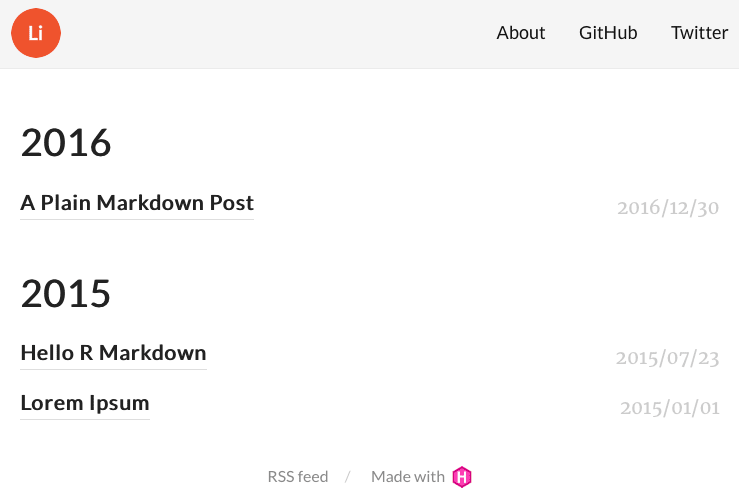
\includegraphics[width=0.9\linewidth]{images/lithium-theme} 

}

\caption{La página de inicio del nuevo sitio por defecto.}\label{fig:lithium}
\end{figure}

Tiene que saber tres conceptos más básicos para un sitio web basado en
Hugo:

\begin{enumerate}
\def\labelenumi{\arabic{enumi}.}
\item
  El archivo de configuración \texttt{config.toml}\index{config.toml},
  en el que puede especificar algunas configuraciones globales para su
  sitio. Incluso si no sabe qué es TOML en este momento (se presentará
  en el capítulo \ref{hugo}), aún podrá cambiar algunas configuraciones
  obvias. Por ejemplo, puede ver configuraciones como estas en
  \texttt{config.toml}:

\begin{Shaded}
\begin{Highlighting}[]
\NormalTok{baseurl }\OperatorTok{=} \StringTok{"/"}
\NormalTok{languageCode }\OperatorTok{=} \StringTok{"en-us"}
\NormalTok{title }\OperatorTok{=} \StringTok{"A Hugo website"}
\NormalTok{theme }\OperatorTok{=} \StringTok{"hugo-lithium-theme"}

\NormalTok{[[}\VariableTok{menu}\NormalTok{.}\AttributeTok{main}\NormalTok{]]}
\NormalTok{    name }\OperatorTok{=} \StringTok{"About"}
\NormalTok{    url }\OperatorTok{=} \StringTok{"/about/"}
\NormalTok{[[}\VariableTok{menu}\NormalTok{.}\AttributeTok{main}\NormalTok{]]}
\NormalTok{    name }\OperatorTok{=} \StringTok{"GitHub"}
\NormalTok{    url }\OperatorTok{=} \StringTok{"https://github.com/rstudio/blogdown"}
\NormalTok{[[}\VariableTok{menu}\NormalTok{.}\AttributeTok{main}\NormalTok{]]}
\NormalTok{    name }\OperatorTok{=} \StringTok{"Twitter"}
\NormalTok{    url }\OperatorTok{=} \StringTok{"https://twitter.com/rstudio"}
\end{Highlighting}
\end{Shaded}

  Puede cambiar el título de la página web, e.g.,
  \texttt{title\ =\ "Mi\ propia\ página\ web\ chévere"}, y actualizar
  las URL de GitHub y Twitter.\index{Directories}
\item
  El directorio de contenido (por defecto, \texttt{content/}). Aquí es
  donde usted escribe los archivos de origen R Markdown o Markdown para
  sus publicaciones y páginas. Bajo \texttt{content/} del sitio
  predeterminado, puede ver \texttt{about.md} y un
  directorio\texttt{post/} que contiene algunas publicaciones. La
  organización del directorio de contenido depende de usted. Puede tener
  archivos y directorios arbitrarios allí, según la estructura del sitio
  web que desee.
\item
  El directorio de publicación (por defecto, \texttt{public/}). Su sitio
  web se generará en este directorio, lo que significa que no necesita
  agregar manualmente ningún archivo a este directorio.\footnote{Ejecutando
    \texttt{serve\_site()} o \texttt{build\_site()}, los archivos se
    generarán y publicarán en su directorio de publicación
    automáticamente.} Por lo general, contiene una gran cantidad de
  archivos \texttt{*.html} y dependencias como \texttt{*.css},
  \texttt{*.js} e imágenes. Puede cargar todo en \texttt{public/} a
  cualquier servidor web que pueda publicar sitios web estáticos, y su
  sitio web estará en funcionamiento. Hay muchas opciones para publicar
  sitios web estáticos, y hablaremos más sobre ellos en el capítulo
  \ref{implementación} si no está familiarizado con la implementación de
  sitios web.
\end{enumerate}

Si está satisfecho con este tema predeterminado, ¡está básicamente listo
para comenzar a escribir y publicar su nuevo sitio web! Mostraremos cómo
usar otros temas en la sección \ref{otros-temas}. Sin embargo, tenga en
cuenta que un tema más complicado y elegante puede requerir que aprenda
más sobre todas las tecnologías subyacentes, como el lenguaje de
plantillas de Hugo, HTML, CSS y JavaScript.

\hypertarget{rstudio-ide}{%
\section{RStudio IDE}\label{rstudio-ide}}

Hay algunos complementos básicos de
RStudio\index{Complementos de RStudio} para facilitar la edición y la
vista previa de su sitio web, y puede encontrarlos en el menú ``Addins''
en la barra de herramientas de RStudio:

\begin{itemize}
\item
  ``Serve Site'': este complemento llama a
  \texttt{blogdown::serve\_site()} para presentar continuamente su sitio
  web localmente utilizando la tecnología LiveReload, para que pueda ver
  en vivo el sitio web. Puede seguir editando material para su sitio
  mientras lo está viendo, pero esta función bloqueará su consola de R
  de manera predeterminada, lo que significa que no podrá usar su
  consola de R una vez que inicie este servidor web local. Para
  desbloquear la consola, haga clic en el signo de stop rojo en la
  esquina superior derecha de la ventana de la consola. Si prefiere
  evitar este comportamiento por completo, establezca la opción
  \texttt{options(servr.daemon\ =\ TRUE)}, antes de hacer clic en este
  complemento o llame a la función \texttt{serve\_site()}, para que el
  servidor sea demonizado y no bloquee su consola de R.\^{} {[}Hemos
  oído de casos en los que el servidor demonizado bloquea R en Windows.
  Si tiene problemas con el servidor daemonizado, existen tres
  soluciones alternativas, y puede probar una de ellas: (1) instalar el
  paquete \textbf{later} a través de \texttt{install.packages("later")}
  y volver a iniciar el servidor; (2) use el servidor de Hugo (vea la
  sección \ref{livereload}); (3) llame \texttt{blogdown::serve\_site()}
  en una sesión de R separada, y puede obtener una vista previa de su
  sitio web en su navegador web, pero aún puede editar el sitio web en
  RStudio.{]}
\item
  ``New Post'': este complemento proporciona un cuadro de diálogo para
  que ingrese los metadatos de la publicación de su blog, incluidos el
  título, el autor, la fecha, etc. Ver la Figura \ref{fig:new-post} para
  un ejemplo. Este complemento realmente llama a la función
  \texttt{blogdown::new\_post()}, pero hace algunas cosas
  automáticamente:

  \begin{itemize}
  \item
    A medida que escribe el título de la publicación, generará un nombre
    de archivo para usted, y puede editarlo si no le gusta el generado
    automáticamente. De hecho, también puede usar este complemento para
    crear páginas normales en cualquier directorio bajo
    \texttt{content/}. Por ejemplo, si desea agregar una página de
    currículum, puede cambiar el nombre del archivo a \texttt{resume.md}
    del 'post/YYYY-mm-dd-resume.md` predeterminado.
  \item
    Puede seleccionar la fecha desde un widget de calendario
    proporcionado por Shiny.\footnote{Shiny es un paquete R para crear
      aplicaciones web interactivas usando R. Usando este complemento,
      el widget de calendario le permite ver un calendario interactivo
      por mes para seleccionar fechas. Este es un uso simple de Shiny,
      pero puede leer más acerca de las aplicaciones Shiny aquí:
      \url{https://shiny.rstudio.com}.}
  \item
    Esto escaneará las categorías y etiquetas de las publicaciones
    existentes, por lo que cuando quiera ingresar categorías o
    etiquetas, puede seleccionarlas de los menús desplegables o crear
    otras nuevas.
  \item
    Después de crear una nueva publicación, se abrirá automáticamente,
    por lo que puede comenzar a escribir el contenido de inmediato.
  \end{itemize}
\item
  ``Update Metadata'': Este complemento le permite actualizar los
  metadatos YAML de la publicación abierta actualmente. Ver la Figura
  @ref(fig: update-meta) para un ejemplo. La principal ventaja de este
  complemento es que puede seleccionar categorías y etiquetas de los
  menús desplegables en lugar de tener que recordarlas.
\end{itemize}

\begin{figure}

{\centering 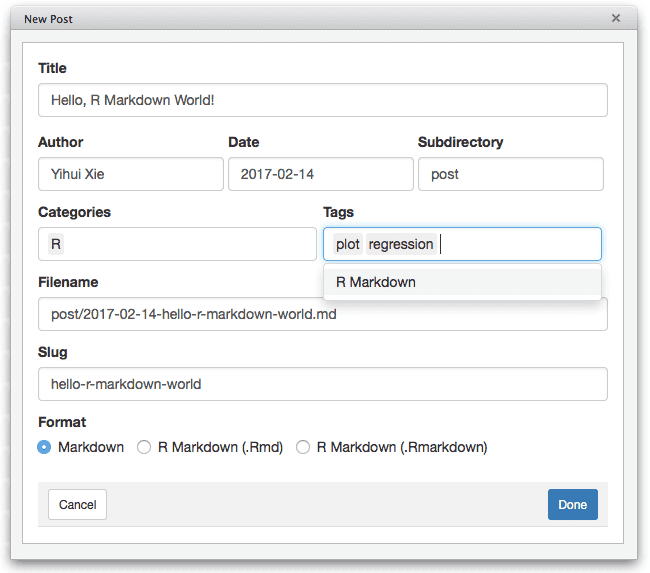
\includegraphics[width=0.8\linewidth]{images/new-post} 

}

\caption{Crear una nueva publicación usando el complemento de RStudio.}\label{fig:new-post}
\end{figure}

\begin{figure}

{\centering 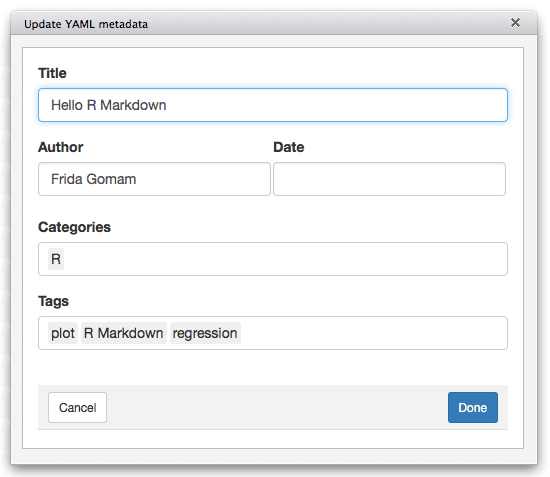
\includegraphics[width=0.7\linewidth]{images/update-meta} 

}

\caption{Actualizar los metadatos de una publicación existente usando el complemento de RStudio.}\label{fig:update-meta}
\end{figure}

Con estos complementos, rara vez deberá ejecutar los comandos en R
manualmente después de haber configurado su sitio web, ya que todas sus
publicaciones se compilarán automáticamente cada vez que cree una nueva
publicación o modifique una existente debido a la función LiveReload.

Si su versión de RStudio es por lo menos la v1.1.383,\footnote{Puede
  descargar todas las versiones del sitio oficial de RStudio incluyendo
  la v1.1.383 desde
  \url{https://www.rstudio.com/products/rstudio/download/}.} puede
actualmente crear un proyecto de página web directamente desde el menú
\texttt{File\ -\textgreater{}\ New\ Project\ -\textgreater{}\ New\ Directory}
(vea la Figura \ref{fig:new-project} y \ref{fig:blogdown-project}).

\begin{figure}

{\centering 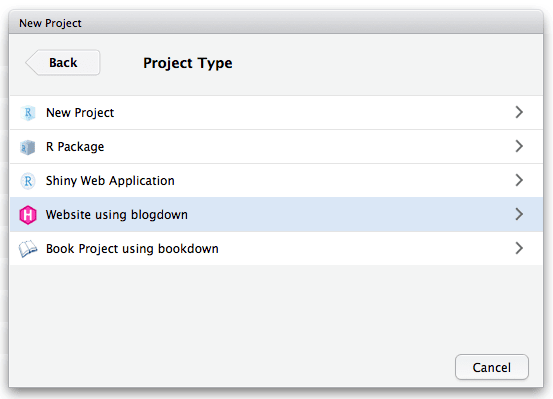
\includegraphics[width=0.8\linewidth]{images/new-project} 

}

\caption{Crear un nuevo proyecto de página web en RStudio.}\label{fig:new-project}
\end{figure}

\begin{figure}

{\centering 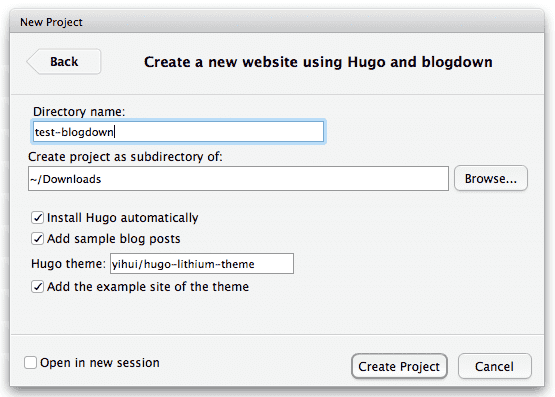
\includegraphics[width=0.8\linewidth]{images/blogdown-project} 

}

\caption{Crear un proyecto de página web basado en blogdown.}\label{fig:blogdown-project}
\end{figure}

Si su sitio web se creó utilizando la función
\texttt{blogdown::new\_site()} en lugar del menú de RStudio por primera
vez, puede salir de RStudio y volver a abrir el proyecto. Si accede al
menú \texttt{Tools\ -\textgreater{}\ Project\ Options}, su tipo de
proyecto debería ser ``Website'' como lo puede ver en la Figura
\ref{fig:project-options}.

Luego verá un panel en RStudio llamado ``Build'' y hay un botón ``Build
Website''. Al hacer clic en este botón, RStudio llamará a
\texttt{blogdown::build\_site\ ()} para construir el sitio web. Esto
generará automáticamente archivos en el directorio
\texttt{public/}.\footnote{O donde sea que esté ubicado su directorio de
  publicación. Es \texttt{public/} de forma predeterminada, pero se
  puede cambiar especificando \texttt{publishDir\ ="myNewDirectory"} en
  el archivo \texttt{config.toml}.} Si desea compilar el sitio web y
publicar los archivos de salida en \texttt{public/} manualmente, se
recomienda reiniciar su sesión de R y hacer clic en este botón ``Build
Website'' antes de publicar el sitio web, en lugar de publicar la
carpeta \texttt{public/} generada de forma continua y automática por
\texttt{blogdown::serve\_site()}, porque este último llama a
\texttt{blogdown::build\_site(local\ =\ TRUE)}, que tiene algunas
diferencias sutiles con \texttt{blogdown::build\_site(local\ =\ FALSE)}
(ver la sección \ref{local-preview} para más detalles).

Recomendamos mucho que desmarque la opción ``Preview site after
building'' en las opciones de proyecto de RStudio (Figura
\ref{fig:project-options}).\footnote{En caso de que se pregunte por qué:
  a menos que haya establecido la opción \texttt{relativeurls} a
  \texttt{true} en \texttt{config.toml}, requiere un servidor web para
  obtener una vista previa del sitio local, de lo contrario, incluso si
  puede ver la página de inicio de su sitio web en RStudio Viewer, la
  mayoría de los enlaces como los enlaces a archivos CSS y JavaScript
  son poco probables que funcionen. Cuando RStudio Viewer le muestra la
  vista previa, en realidad no ejecuta un servidor web.} También puede
desmarcar la opción ``Re-knit current preview when supporting files
change'', ya que esta opción no es realmente útil después de llamar a
\texttt{serve\_site()}.

\begin{figure}

{\centering 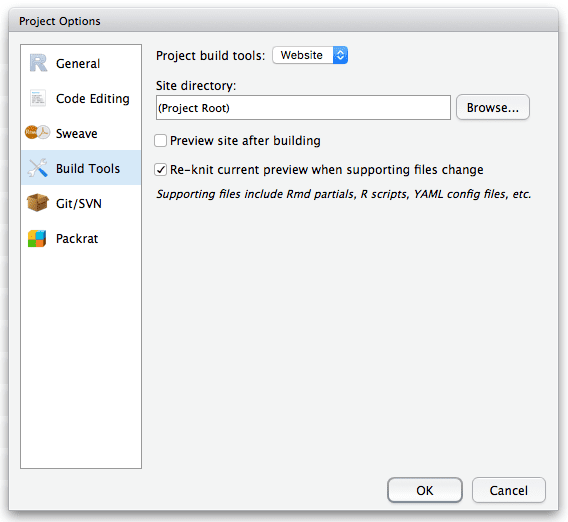
\includegraphics[width=0.8\linewidth]{images/project-options} 

}

\caption{Opciones de proyecto de RStudio.}\label{fig:project-options}
\end{figure}

\hypertarget{opciones-globales}{%
\section{\texorpdfstring{Opciones
globales\index{Global Options}}{Opciones globales}}\label{opciones-globales}}

Dependiendo de sus preferencias personales, puede establecer algunas
opciones globales antes de trabajar en su sitio web. Estas opciones se
deben configurar usando \texttt{options(name\ =\ value)}, y las opciones
disponibles actualmente se presentan en Table \ref{tab:global-options}.

\begin{table}

\caption{\label{tab:global-options}Opciones globales que afectan el comportamiento de blogdown.}
\centering
\begin{tabular}[t]{lll}
\toprule
Option name & Default & Meaning\\
\midrule
servr.daemon & FALSE & Si debe usar un servidor demonizado\\
blogdown.author &  & El autor por defecto de nuevas publicaciones\\
blogdown.ext & .md & Extensión por defecto de nuevas publicaciones\\
blogdown.subdir & post & Un subdirectorio bajo content/\\
blogdown.yaml.empty & TRUE & Preservar campos vacíos en YAML?\\
\bottomrule
\end{tabular}
\end{table}

Le recomendamos que configure estas opciones en su archivo de perfil de
inicio de R. Puede consultar la página de ayuda \texttt{?Rprofile} para
más detalles, y aquí hay una introducción simplificada. Un archivo de
perfil de inicio es básicamente un script en R que se ejecuta cuando se
inicia la sesión de R. Este es un lugar perfecto para establecer
opciones globales, por lo que no necesita escribir estas opciones
nuevamente cada vez que inicie una nueva sesión en R. Puede usar un
archivo de perfil global \texttt{\textasciitilde{}/.Rprofile},\footnote{La
  tilde \texttt{\textasciitilde{}} indica el directorio principal en su
  sistema.} O un archivo por proyecto \texttt{.Rprofile} en el
directorio raíz de su proyecto de RStudio. El primero se aplicará a
todas las sesiones de R que inicie, a menos que haya proporcionado el
último para anularlo. La forma más fácil de crear un archivo de este
tipo es usar \texttt{file.edit()} en RStudio, por ejemplo,

\begin{Shaded}
\begin{Highlighting}[]
\KeywordTok{file.edit}\NormalTok{(}\StringTok{'~/.Rprofile'}\NormalTok{)}
\CommentTok{# o file.edit('.Rprofile')}
\end{Highlighting}
\end{Shaded}

Supongamos que siempre prefiere el servidor demonizado y quiere que el
autor de las nuevas publicaciones sea ``John Doe'' de manera
predeterminada. Puede establecer estas opciones en el archivo de perfil:

\begin{Shaded}
\begin{Highlighting}[]
\KeywordTok{options}\NormalTok{(}\DataTypeTok{servr.daemon =} \OtherTok{TRUE}\NormalTok{, }\DataTypeTok{blogdown.author =} \StringTok{'John Doe'}\NormalTok{)}
\end{Highlighting}
\end{Shaded}

Una buena consecuencia de establecer estas opciones es que cuando usa el
complemento de RStudio ``New post'', los campos ``Author'',
``Subdirectory'' y ``Format'' se completarán automáticamente, por lo que
no tendrá que manipularlos todas las veces a menos que desea cambiar los
valores predeterminados (ocasionalmente).

R solo lee un archivo de perfil de inicio. Por ejemplo, si tiene un
\texttt{.Rprofile} en el directorio actual y un
\texttt{\textasciitilde{}/.Rprofile} global, solo el anterior se
ejecutará cuando R se inicie desde el directorio actual. Esto puede
hacer que sea inconveniente para varios autores que colaboran en el
mismo proyecto de un sitio web, ya que no puede establecer opciones
específicas del autor. En particular, no es posible establecer la opción
\texttt{blogdown.author} en un solo \texttt{.Rprofile}, porque esta
opción debería ser diferente para diferentes autores. Una solución
consiste en establecer opciones comunes en \texttt{.Rprofile} bajo del
directorio raíz del proyecto del sitio web, y también ejecutar el
\texttt{\textasciitilde{}/.Rprofile} global si existe. Las opciones
específicas del autor se pueden establecer en el
\texttt{\textasciitilde{}/.Rprofile} global en la computadora de cada
autor.

\begin{Shaded}
\begin{Highlighting}[]
\CommentTok{# en el .Rprofile del proyecto de la página web}
\ControlFlowTok{if}\NormalTok{ (}\KeywordTok{file.exists}\NormalTok{(}\StringTok{'~/.Rprofile'}\NormalTok{)) \{}
\NormalTok{  base}\OperatorTok{::}\KeywordTok{sys.source}\NormalTok{(}\StringTok{'~/.Rprofile'}\NormalTok{, }\DataTypeTok{envir =} \KeywordTok{environment}\NormalTok{())}
\NormalTok{\}}
\CommentTok{# luego configure options(blogdown.author = 'Your Name') en ~/.Rprofile}
\end{Highlighting}
\end{Shaded}

\hypertarget{output-format}{%
\section{R Markdown vs.~Markdown}\label{output-format}}

Si no está familiarizado con R Markdown \index{R Markdown}, consulte el
Apéndice \ref{r-markdown} para obtener un tutorial rápido. Cuando crea
una nueva publicación, debe decidir si desea usar R Markdown o Markdown
simple \index{Markdown}, como puede ver en Figure \ref{fig:new-post}.
Las principales diferencias son:

\begin{enumerate}
\def\labelenumi{\arabic{enumi}.}
\item
  No puede ejecutar ningún código en R en un documento de Markdown
  simple, mientras que en un documento de Markdown R, puede incrustar
  fragmentos de código R
  (\texttt{\textasciigrave{}\textasciigrave{}\textasciigrave{}\{r\}}).
  Sin embargo, aún puede incrustar código de R en Markdown simple usando
  la sintaxis para bloques de código delimitados
  \texttt{\textasciigrave{}\textasciigrave{}\textasciigrave{}r}(tenga en
  cuenta que no hay llaves \texttt{\{\}}). Tales bloques de código no se
  ejecutarán y pueden ser adecuados para propósitos de demostración
  pura. A continuación se muestra un ejemplo de un fragmento de código
  de R en R Markdown:

\begin{Shaded}
\begin{Highlighting}[]
\NormalTok{```\{r cool-plot, fig.width='80%', fig.cap='A cool plot.'\}}
\NormalTok{plot(cars, pch = 20)  # no es muy chévere}
\NormalTok{```}
\end{Highlighting}
\end{Shaded}

  Y aquí hay un ejemplo de un bloque de código de R en Markdown simple:

\begin{Shaded}
\begin{Highlighting}[]
\NormalTok{```r}
\NormalTok{1 + 1  # no ejecutada}
\NormalTok{```}
\end{Highlighting}
\end{Shaded}
\item
  Una publicación en Markdown simple es ejecutada en HTML a través de
  \href{https://gohugo.io/overview/configuration/}{Blackfriday}
  \index{Blackfriday}(un paquete escrito en lenguaje Go y adoptado por
  Hugo). Un documento R Markdown se compila a través de los paquetes
  \textbf{rmarkdown}, \textbf{bookdown}, y Pandoc\index{Pandoc}, lo que
  significa que puede usar la mayoría de las características de
  \href{http://pandoc.org/MANUAL.html\#pandocs-markdown}{Markdown de
  Pandoc} y
  \href{https://bookdown.org/yihui/bookdown/components.html}{extensiones
  de Markdown para \textbf{bookdown}} en \textbf{blogdown}. Si usa R
  Markdown \citep{R-rmarkdown} con \textbf{blogdown}, le recomendamos
  que lea la documentación de Pandoc y \textbf{bookdown} al menos una
  vez para conocer todas las características posibles. No repetiremos
  los detalles en este libro, pero enumeraremos las características
  brevemente a continuación, que también se muestran en el sitio web de
  ejemplo: \url{https://blogdown-demo.rbind.io}.

  \begin{itemize}
  \item
    Formateo en línea: texto en \texttt{\_italica\_} /
    \texttt{**negrita**} y
    \texttt{\textasciigrave{}código\ en\ línea\textasciigrave{}}.
  \item
    Elementos en línea: subíndices (e.g.,
    \texttt{H\textasciitilde{}2\textasciitilde{}0}) y superíndices
    (e.g., \texttt{R\^{}2\^{}}); links (\texttt{{[}texto{]}(url)}) e
    imágenes \texttt{!{[}título{]}(url)}; notas al pie
    \texttt{texto\^{}{[}nota\ al\ pie{]}}.
  \item
    Elementos de nivel bloque: párrafos; encabezados de sección
    numerados y no numerados; listas ordenadas y no ordenadas; citas en
    bloque; bloques de código; tablas; reglas horizontales.
  \item
    Expresiones matemáticas y ecuaciones.
  \item
    Teoremas y demostraciones.
  \item
    Bloques de código en R que se pueden usar para producir salida de
    texto (incluidas tablas) y gráficos. Tenga en cuenta que las
    ecuaciones, teoremas, tablas y figuras se pueden numerar y
    referenciadas cruzadamente.
  \item
    Citas y bibliografía.
  \item
    HTML widgets, y aplicaciones en Shiny incrustadas mediante
    \texttt{\textless{}iframe\textgreater{}}.
  \end{itemize}
\end{enumerate}

Hay muchas diferencias en la sintaxis entre el Markdown de Blackfriday y
el Markdown de Pandoc. Por ejemplo, puede escribir una lista de tareas
con Blackfriday, pero no con Pandoc:

\begin{Shaded}
\begin{Highlighting}[]
\NormalTok{- }\FloatTok{[x] Escribir un paquete en R.}
\FloatTok{- [ ] Escribir un libro.}
\FloatTok{- [ ] ...}
\FloatTok{- [ ] Beneficio!}
\end{Highlighting}
\end{Shaded}

Del mismo modo, Blackfriday no admite matemática en LaTeX y Pandoc sí.
Hemos agregado el soporte \href{https://www.mathjax.org/\#docs}{MathJax}
\index {MathJax} al tema predeterminado
(\href{https://github.com/yihui/hugo-lithium-theme}{hugo-lithium-theme}
en \textbf{blogdown} para compilar matemática en LaTeX en páginas HTML,
pero hay una advertencia para las publicaciones simples de Markdown:
debe incluir expresiones matemáticas en línea con un par de comillas
\texttt{\textasciigrave{}\$math\$\textasciigrave{}}, por ejemplo,
\texttt{\textasciigrave{}\$S\_n\ =\ \textbackslash{}\ um\_\{i=1\}\^{}n\ X\_i\$\textasciigrave{}}.
Del mismo modo, las expresiones matemáticas del estilo de visualización
deben escribirse en
\texttt{\textasciigrave{}\$\$math\$\$\textasciigrave{}}. Para las
publicaciones de R Markdown, puede usar \texttt{\$math\$} para
expresiones matemáticas en línea, y \texttt{\$\$math\$\$} para
expresiones de estilo de visualización.\footnote{El motivo por el que
  necesitamos los respaldos para documentos de Markdown simples es que
  tenemos que evitar que Blackfriday interprete el código LaTeX como
  Markdown. Las comillas asegurarán que el contenido interno no se
  traduzca como Markdown a HTML, por ejemplo,
  \texttt{\textasciigrave{}\$\$x\ *y*\ z\$\$\textasciigrave{}} se
  convertirá en
  \texttt{\textless{}code\textgreater{}\ \$\$x\ *y*\ z\$\$\textless{}/code\textgreater{}}.
  Sin las comillas, se convertirá en
  \texttt{\$\$x\ \textless{}em\textgreater{}y\textless{}/em\textgreater{}\ z\$\$},
  que no es una expresión matemática en LaTeX válida para MathJax.
  Problemas similares pueden surgir cuando tenga otros caracteres
  especiales como guiones bajos en sus expresiones matemáticas.}

Si considera que es un dolor tener que recordar las diferencias entre R
Markdown y Markdown, una opción conservadora es usar siempre R Markdown,
incluso si su documento no contiene ningún fragmento de código en R.
Markdown de Pandoc es mucho más rico que Blackfriday, y solo hay un
pequeño número de características no disponibles en Pandoc pero
presentes en Blackfriday. Las principales desventajas de usar R Markdown
son:

\begin{enumerate}
\def\labelenumi{\arabic{enumi}.}
\item
  Puede sacrificar algo de velocidad en la renderización del sitio web,
  pero esto puede no ser notorio debido a un mecanismo de almacenamiento
  en caché en \textbf{blogdown} (lea más sobre esto en la sección
  \ref{local-preview}). Hugo es muy rápido cuando procesa archivos de
  Markdown simples, y típicamente debería tomar menos de un segundo para
  renderizar unos cientos de archivos de Markdown.
\item
  Tendrá algunos archivos HTML intermedios en el directorio fuente de su
  sitio web, porque \textbf{blogdown} tiene que llamar a
  \textbf{rmarkdown} para renderizar previamente los archivos
  \texttt{*.Rmd} \texttt{*.html}. También tendrá carpetas intermedias
  para las figuras (\texttt{*\_files/}) y la memoria caché
  (\texttt{*\_cache/}) si tiene una salida de trazado en fragmentos de
  código en R o ha habilitado el almacenamiento en cache de
  \textbf{knitr}. A menos que le importe mucho la ``limpieza'' del
  repositorio fuente de su sitio web (especialmente cuando usa una
  herramienta de control de versiones como GIT), estos archivos
  intermedios no deberían importar.
\end{enumerate}

En este libro, generalmente nos referimos a los archivos \texttt{.Rmd}
cuando decimos ``Documentos de R Markdown'', que se compilan a
\texttt{.html} de forma predeterminada. Sin embargo, hay otro tipo de
documento de R Markdown con la extensión de nombre de archivo
\texttt{.Rmarkdown}. Dichos documentos de R Markdown se compilan para
los documentos Markdown con la extensión \texttt{.markdown}, que serán
procesados por Hugo en lugar de por Pandoc. Hay dos limitaciones
principales de usar \texttt{.Rmarkdown} en comparación con\texttt{.Rmd}:

\begin{itemize}
\item
  No puede usar las funciones de reducción solo compatibles con Pandoc,
  como las citas. Las expresiones matemáticas solo funcionan si ha
  instalado el paquete \textbf{xaringan} \citep{R-xaringan} y ha
  aplicado la solución de JavaScript mencionada en la sección
  \ref{javascript}.
\item
  Los widgets HTML no son compatibles.
\end{itemize}

La principal ventaja de usar \texttt{.Rmarkdown} es que los archivos de
salida son más limpios porque son archivos Markdown. Puede ser más fácil
para usted leer la salida de sus publicaciones sin mirar las páginas web
reales renderizadas. Esto puede ser particularmente útil al revisar los
pull requests de GitHub. Tenga en cuenta que las tablas, figuras,
ecuaciones y teoremas numerados también son compatibles. No puede usar
directamente la sintaxis de Markdown en las leyendas de tabla o figura,
pero puede usar referencias de texto como una solución alternativa
(consulte la documentación de \textbf{bookdown}).

Para cualquier documento de R Markdown (no específico de
\textbf{blogdown}), debe especificar un formato de salida. Hay muchos
posibles \href{http://rmarkdown.rstudio.com/lesson-9.html}{formatos de
salida} en el paquete \textbf{rmarkdown} (como \texttt{html\_document} y
\texttt{pdf\_document}) y otros paquetes de extensión (tales como
\texttt{tufte::tufte\_html} y \texttt{bookdown::gitbook}). Por supuesto,
el formato de salida para los sitios web debe ser HTML. Hemos
proporcionado una función de formato de salida
\texttt{blogdown::html\_page} en \textbf{blogdown}, y todos los archivos
R Markdown se renderizan con este formato. Se basa en el formato de
salida \texttt{bookdown::html\_document2}, lo que significa que ha
heredado muchas características de \textbf{bookdown} además de las
características en Pandoc. Por ejemplo, puede numerar y hacer
referencias cruzadas de ecuaciones matemáticas, figuras, tablas y
teoremas, etc. Consulte el Capítulo 2 del libro \textbf{bookdown}
\citep{xie2016} para obtener más detalles sobre la sintaxis.

Note que el formato de salida \texttt{bookdown::html\_document2} a su
vez hereda de \texttt{rmarkdown::html\_document}, entonces necesita ver
la página de ayuda \texttt{?rmarkdown::html\_document} para todas las
opciones posibles para el formato \texttt{blogdown::html\_page}. Si
desea cambiar los valores predeterminados de las opciones de este
formato de salida, puede agregar un campo \texttt{output} a sus
metadatos YAML. Por ejemplo, podemos agregar una tabla de contenido a
una página, establecer el ancho de la figura en 6 pulgadas y usar el
dispositivo \texttt{svg} para los gráficos estableciendo estas opciones
en YAML:

\begin{Shaded}
\begin{Highlighting}[]
\OtherTok{---}
\FunctionTok{title:}\AttributeTok{ }\StringTok{"Mi grandiosa publicación"}
\StringTok{author: "}\ErrorTok{John Doe"}
\FunctionTok{date:}\AttributeTok{ }\StringTok{"2017-02-14"}
\FunctionTok{output:}
  \FunctionTok{blogdown:}\AttributeTok{:html_page:}
    \FunctionTok{toc:}\AttributeTok{ true}
    \FunctionTok{fig_width:}\AttributeTok{ 6}
    \FunctionTok{dev:}\AttributeTok{ }\StringTok{"svg"}
\OtherTok{---}
\end{Highlighting}
\end{Shaded}

Para establecer opciones para \texttt{blogdown::html\_page()}
globalmente (es decir, aplicar ciertas opciones a todos los archivos
Rmd), puede crear un archivo \texttt{\_output.yml} en el directorio raíz
de su sitio web. Este archivo YAML debe contener el formato de salida
directamente (no coloque el formato de salida bajo la opción
\texttt{output}), por ejemplo,

\begin{Shaded}
\begin{Highlighting}[]
\FunctionTok{blogdown:}\AttributeTok{:html_page:}
  \FunctionTok{toc:}\AttributeTok{ true}
  \FunctionTok{fig_width:}\AttributeTok{ 6}
  \FunctionTok{dev:}\AttributeTok{ }\StringTok{"svg"}
\end{Highlighting}
\end{Shaded}

Por el momento, no todas las funciones de
\texttt{rmarkdown::html\_document} son compatibles con
\textbf{blogdown}, como \texttt{df\_print},
\texttt{code\_folding},\texttt{code\_download}, etc.

Si su trozo de código tiene salida de gráficos, le recomendamos que
evite caracteres especiales como espacios en la etiqueta de fragmentos.
Lo ideal es que solo use caracteres alfanuméricos y guiones, por
ejemplo,
\texttt{\textasciigrave{}\textasciigrave{}\textasciigrave{}\{r,\ my-label\}}
en lugar de
\texttt{\textasciigrave{}\textasciigrave{}\textasciigrave{}\{r,\ my\ label\}}.

No se recomienda cambiar las opciones \textbf{knitr} chunk
\texttt{fig.path} o \texttt{cache.path} en R Markdown. Los valores
predeterminados de estas opciones funcionan mejor con \textbf{blogdown}.
Lea la sección \ref{dep-path} para conocer los motivos técnicos, si lo
prefiere.

Si está trabajando en una publicación de R Markdown, pero no quiere que
\textbf{blogdown} la compile, puede cambiar temporalmente su extensión
de nombre de archivo de \texttt{.Rmd} a otra extensión desconocida como
\texttt{.Rmkd}.

\hypertarget{otros-temas}{%
\section{Otros temas}\label{otros-temas}}

En Hugo, los temas \index{Temas} controlan toda la apariencia y
funcionalidad de su sitio. Entonces, si le importa mucho el aspecto de
su sitio web, probablemente pasará bastante tiempo al principio buscando
un tema de Hugo que le guste de la colección que figura en
\url{http://themes.gohugo.io}. Tenga en cuenta que no todos los temas se
han probado en \textbf{blogdown}. Si encuentra que un determinado tema
no funciona bien con \textbf{blogdown}, puede informar a
\url{https://github.com/rstudio/blogdown/issues}, e intentaremos
investigar el motivo, pero puede ser una cuestión de tiempo aprender y
comprender cómo funciona un nuevo tema, por lo que le recomendamos que
aprenda más acerca de Hugo por su cuenta antes de preguntar, y también
alentamos a los usuarios a ayudarse mutuamente allí.

Después de haber encontrado un tema satisfactorio, debe averiguar su
nombre de usuario y el nombre del repositorio de GitHub,\footnote{Para
  la mayoría de los temas, puede encontrar esto navegando al tema de su
  elección desde \url{http://themes.gohugo.io} y luego haciendo clic en
  \texttt{Homepage}.} luego instale el tema a través
de\index{blogdown::install\_theme()}
\texttt{blogdown::install\_theme()}, o simplemente cree un nuevo sitio
bajo otro directorio nuevo y pase el nombre del repositorio de GitHub al
argumento \texttt{theme} de \texttt{new\_site()}. Recomendamos que use
el segundo enfoque, porque los temas de Hugo podrían ser muy complicados
y el uso de cada tema puede ser muy diferente y muy dependiente del
\texttt{config.toml}. Si instala un tema con \texttt{install\_theme()}
en lugar de \texttt{new\_site\ ()}, deberá crear manualmente el archivo
\texttt{config.toml} en el directorio raíz de su sitio web para que
coincida con el tema recién instalado.\footnote{Una solución
  alternativa, si usó \texttt{install\_theme()} y establece el argumento
  \texttt{theme\_example} en TRUE, entonces puede acceder a un archivo
  \texttt{config.toml} de ejemplo. En el directorio \texttt{themes/},
  vaya al archivo del tema que acaba de descargar y busque
  \texttt{exampleSite/config.toml}. Este archivo puede copiarse en su
  directorio raíz (para reemplazar el archivo \texttt{config.toml} de su
  tema original) o usarse como una plantilla para escribir correctamente
  un nuevo archivo \texttt{config.toml} para su nuevo tema.}

\begin{Shaded}
\begin{Highlighting}[]
\CommentTok{# por ejemplo, cree un sitio nuevo con el tema academic}
\NormalTok{blogdown}\OperatorTok{::}\KeywordTok{new_site}\NormalTok{(}\DataTypeTok{theme =} \StringTok{'gcushen/hugo-academic'}\NormalTok{)}
\end{Highlighting}
\end{Shaded}

Para ahorrarle tiempo, enumeramos algunos temas a continuación que
coinciden con nuestro gusto:

\begin{itemize}
\item
  Temas Simples/mínimos:
  \href{https://github.com/yihui/hugo-xmin}{XMin,}
  \href{https://github.com/road2stat/hugo-tanka}{Tanka,}
  \href{https://github.com/AlexFinn/simple-a}{simple-a,} and
  \href{https://github.com/jbub/ghostwriter}{ghostwriter.}
\item
  Temas sofisticados:
  \href{https://github.com/gcushen/hugo-academic}{hugo-academic}
  (fuertemente recomendado para usuarios de la academia),
  \href{https://github.com/kakawait/hugo-tranquilpeak-theme}{hugo-tranquilpeak-theme,}
  \href{https://github.com/kishaningithub/hugo-creative-portfolio-theme}{hugo-creative-portfolio-theme,}
  and
  \href{https://github.com/devcows/hugo-universal-theme}{hugo-universal-theme.}
\item
  Temas que contienen multimedia: Si está interesado en agregar
  contenido multimedia a su sitio (como archivos de audio de un
  podcast), el tema
  \href{https://github.com/mattstratton/castanet}{castanet} proporciona
  un excelente marco adaptado para esta aplicación. Un ejemplo de un
  sitio que usa \textbf{blogdown} con el tema castanet es
  \href{https://www.r-podcast.org}{R-Podcast}
\end{itemize}

Si no entiende HTML, CSS o JavaScript, y no tiene experiencia con los
temas o plantillas de Hugo, puede tardar unos 10 minutos en comenzar a
usar su nuevo sitio web, ya que debe aceptar todo lo que le ofrecen
(como el tema predeterminado); Si tiene el conocimiento y la experiencia
(y desea personalizar su sitio al máximo), puede tardar varios días en
comenzar. Hugo es realmente poderoso. Tenga cuidado con el poder.

Otra cosa a tener en cuenta es que cuanto más esfuerzo hagas en un tema
complicado, más difícil será cambiar a otros temas en el futuro, porque
es posible que haya personalizado muchas cosas que no son fáciles de
transferir a otro tema. Por lo tanto, pregúntese seriamente: ``¿Me gusta
tanto este tema tan elegante que definitivamente no lo cambiaré en los
próximos años?''.

\begin{quote}
Si elige cavar un hoyo bastante profundo, algún día no tendrá más
remedio que seguir cavando, incluso con lágrimas.

\VA{--- Liyun Chen\footnote{Traducido de su weibo Chino:
  \url{http://weibo.com/1406511850/Dhrb4toHc} (no puede ver esta página
  a menos que haya iniciado sesión).}}{}
\end{quote}

\hypertarget{workflow}{%
\section{Un flujo de trabajo recomendado}\label{workflow}}

Hay muchas maneras de comenzar a construir un sitio web y presentarlo.
Debido a la gran cantidad de tecnologías que necesita aprender para
comprender completamente cómo funciona un sitio web, nos gustaría
recomendar un flujo de trabajo a los principiantes, por lo que es de
esperar que no necesiten digerir el resto de este libro. Definitivamente
este no es el flujo de trabajo más óptimo, pero requiere que conozca la
menor cantidad de detalles técnicos.

Para comenzar un nuevo sitio web:

\begin{enumerate}
\def\labelenumi{\arabic{enumi}.}
\item
  Elija cuidadosamente un tema en \url{http://themes.gohugo.io}, y
  encuentre el enlace a su repositorio GitHub, que tiene la forma
  \texttt{https://github.com/user/repo}.
\item
  Cree un nuevo proyecto en RStudio y escriba el código
  \texttt{blogdown::new\_site\ (theme\ =\ \textquotesingle{}user/repo\textquotesingle{})}
  en la consola R, donde \texttt{user/repo} proviene del enlace en el
  paso 1.
\item
  Juegue con el nuevo sitio por un tiempo y si no le gusta, puede
  repetir los pasos anteriores, de lo contrario edite las opciones en
  \texttt{config.toml}. Si no comprende ciertas opciones, vaya a la
  documentación del tema, que a menudo es la página README del
  repositorio de GitHub. No todas las opciones tienen que ser cambiadas.
\end{enumerate}

Para editar una página web:

\begin{enumerate}
\def\labelenumi{\arabic{enumi}.}
\item
  Establezca \texttt{options(servr.daemon\ =\ TRUE)} a menos que ya lo
  haya configurado en \texttt{.Rprofile}. Si esta opción no funciona
  para usted (por ejemplo, bloquea su sesión en R), consulte la sección
  \ref{opciones-globales} para obtener una solución alternativa.
\item
  Haga clic en el complemento de RStudio ``Serve Site'' para obtener una
  vista previa del sitio en RStudio Viewer. Esto solo debe hacerse una
  vez cada vez que abra el proyecto RStudio o reinicie su sesión en R.
  No haga clic en el botón knit en la barra de herramientas de RStudio.
\item
  Use el complemento ``New Post'' para crear una nueva publicación o
  página, luego empiece a escribir el contenido.
\item
  Use el complemento ``Update Metadata'' para modificar los metadatos
  del YAML, si es necesario.
\end{enumerate}

Para publicar un sitio web, si no está familiarizado con GIT o GitHub:

\begin{enumerate}
\def\labelenumi{\arabic{enumi}.}
\item
  Reinicie la sesión de R, y ejecute \texttt{blogdown::hugo\_build()}.
  Debería obtener un directorio \texttt{public/} bajo el directorio raiz
  de su proyecto.
\item
  Inicie sesión en\index{Netlify} \url{https://www.netlify.com} (puede
  usar una cuenta de GitHub, si la tiene). Si esta es la primera vez que
  publica este sitio web, puede crear un sitio nuevo; de lo contrario,
  puede actualizar el sitio existente que creó la última vez. Puede
  arrastrar y soltar la carpeta \texttt{public/} desde su visor de
  archivos al área indicada en la página web de Netlify, donde dice
  ``Drag a folder with a static site here''.
\item
  Espere unos segundos para que Netlify despliegue los archivos y le
  asignará un subdominio aleatorio de la forma
  \texttt{random-word-12345.netlify.com}. Puede (y debería) cambiar este
  subdominio aleatorio a uno más significativo si todavía está
  disponible.
\end{enumerate}

Puede ser mucho más fácil publicar un sitio web si está familiarizado
con GIT y GitHub. Recomendamos que cree un nuevo sitio en Netlify desde
su repositorio de GitHub que contenga los archivos fuente de su sitio
web, para que pueda disfrutar los beneficios de la implementación
continua en lugar de cargar manualmente la carpeta \texttt{public/} cada
vez. Con este enfoque, no es necesario ejecutar
\texttt{blogdown::hugo\_build()} localmente, ya que el sitio web se
puede construir en Netlify a través de Hugo. Consulte el capítulo
\ref{implementación} para obtener más información.

\hypertarget{hugo}{%
\chapter{Hugo}\label{hugo}}

En este capítulo, presentaremos brevemente\index{Hugo} Hugo
(\url{https://gohugo.io}), el generador de sitios estáticos en el que se
basa \textbf{blogdown}. Este capítulo no pretende reemplazar la
documentación oficial de Hugo, sino proporcionar una guía para aquellos
que recién están comenzando con Hugo. En caso de duda, consulte la
documentación oficial de Hugo.

\hypertarget{static-sites}{%
\section{Sitios estáticos y Hugo}\label{static-sites}}

Un sitio estático\index{Sitio estático} a menudo consiste en archivos
HTML (con dependencias externas opcionales como imágenes y bibliotecas
de JavaScript), y el servidor web envía exactamente el mismo contenido
al navegador web sin importar quién visita las páginas web. No hay
computación dinámica en el servidor cuando se solicita una página. En
contraste, un sitio dinámico se basa en un lenguaje del lado del
servidor para hacer cierta informática y envía contenido potencialmente
diferente dependiendo de las diferentes condiciones. Un lenguaje común
es PHP, y un ejemplo típico de un sitio dinámico es un foro web. Por
ejemplo, cada usuario tiene una página de perfil, pero generalmente esto
no significa que el servidor haya almacenado una página de perfil HTML
diferente para cada usuario. En cambio, el servidor obtendrá los datos
del usuario de una base de datos y renderizará la página de perfil de
forma dinámica.

Para un sitio estático, cada URL que visita a menudo tiene un archivo
HTML correspondiente almacenado en el servidor, por lo que no es
necesario calcular nada antes de presentar el archivo a los visitantes.
Esto significa que los sitios estáticos tienden a ser más rápidos en
tiempo de respuesta que los sitios dinámicos, y también son mucho más
fáciles de implementar, ya que la implementación simplemente significa
copiar archivos estáticos a un servidor. Un sitio dinámico a menudo se
basa en bases de datos, y tendrá que instalar más paquetes de software
para presentar un sitio dinámico. Para obtener más ventajas de los
sitios estáticos, lea la
\href{https://gohugo.io/overview/introduction/}{introducción} en el
sitio web de Hugo.

Existen muchos generadores de sitios estáticos existentes, incluyendo
Hugo, \href{http://jekyllrb.com}{Jekyll,} y
\href{https://hexo.io}{Hexo,} etc. La mayoría de ellos puede construir
sitios web de propósito general, pero a menudo se utilizan para
construir blogs.

Amamos a Hugo por muchas razones, pero hay algunas que se destacan. A
diferencia de otros generadores de sitios estáticos, la instalación de
Hugo es muy simple porque proporciona un único archivo ejecutable sin
dependencias para la mayoría de los sistemas operativos (consulte la
sección \ref{instalación}). También se diseñó para procesar cientos de
páginas de contenido más rápido que los generadores de sitios estáticos
comparables y, según los informes, puede presentar una página en
aproximadamente 1 milisegundo. Por último, la comunidad de usuarios de
Hugo es muy activa tanto en el \href{https://discuss.gohugo.io}{foro de
discusión de Hugo} y en los
\href{https://github.com/gohugoio/hugo/issues}{issues de GitHub.}

Aunque creemos que Hugo es un fantástico generador de sitios estáticos,
en realidad hay una única característica importante que falta: el
soporte para R Markdown. Ese es básicamente el objetivo del paquete
\textbf{blogdown}.\footnote{Otra motivación fue una manera más fácil de
  crear nuevas páginas o publicaciones. Los generadores de sitios
  estáticos a menudo proporcionan comandos para crear nuevas
  publicaciones, pero a menudo tiene que abrir y modificar el nuevo
  archivo creado a mano después de usar estos comandos. Estaba muy
  frustrado por esto, porque estaba buscando una interfaz gráfica de
  usuario donde simplemente pudiera completar el título, el autor, la
  fecha y otra información sobre una página, luego poder comenzar a
  escribir el contenido de inmediato. Es por eso que proporcioné el
  complemento de RStudio ``New Post'' y la función
  \texttt{blogdown::new\_post()}. En los últimos años, lo odié cada vez
  que estaba a punto de crear una nueva publicación, ya sea a mano o a
  través de la línea de comandos de Jekyll. Finalmente, me volví adicto
  a los blogs una vez que terminé el complemento de RStudio.} Esta
función faltante significa que no puede generar resultados fácilmente
usando el código de R en sus páginas web, ya que solo puede usar
documentos estáticos de Markdown. Además, el motor de Markdown
predeterminado de Hugo es ``Blackfriday'', que es menos poderoso que
Pandoc.\footnote{El soporte de Pandoc se ha agregado en un pull request
  de Hugo: \url{https://github.com/gohugoio/hugo/pull/4060}. Sin
  embargo, creo que el soporte es bastante limitado, y le recomiendo que
  use el formato R Markdown, porque con el soporte oficial de Pandoc en
  Hugo, no puede personalizar las opciones de la línea de comandos de
  Pandoc, la renderización no está en caché (podría ser lento), y no
  podrá usar ninguna extensión de Markdown del paquete \textbf{bookdown}
  (como la numeración de los títulos de las figuras).}

Hugo usa una estructura especial de archivos y carpetas para crear su
sitio web (Figura \ref{fig:folders}). El resto de este capítulo brindará
más detalles sobre los siguientes archivos y carpetas:

\begin{itemize}
\tightlist
\item
  \texttt{config.toml}
\item
  \texttt{content/}
\item
  \texttt{static/}
\item
  \texttt{themes/}
\item
  \texttt{layouts/}
\end{itemize}




\begin{figure}

{\centering 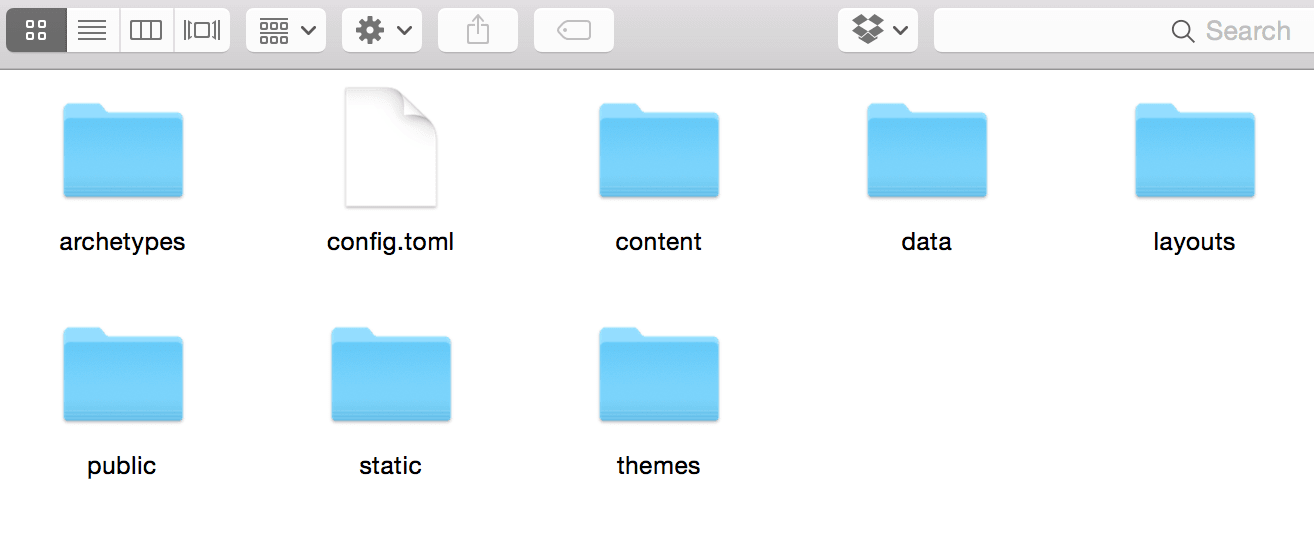
\includegraphics[width=1\linewidth]{images/folder-structure} 

}

\caption{Posibles archivos y carpetas creados cuando crea un nuevo
sitio usando \textbf{blogdown}.}\label{fig:folders}
\end{figure}

\hypertarget{configuracion}{%
\section{Configuración}\label{configuracion}}

El primer archivo que puede ver es el archivo
configuration\index{config.toml} o \texttt{config} en su directorio
raíz, en el que puede establecer configuraciones globales de su sitio.
Puede contener opciones como el título y la descripción de su sitio, así
como otras opciones globales como enlaces a sus redes sociales, el menú
de navegación y la URL base de su sitio web.

Al generar su sitio, Hugo buscará primero un archivo llamado
\texttt{config.toml}. Si no puede encontrar uno, continuará buscando
\texttt{config.yaml}.\footnote{Hugo también admite \texttt{config.json},
  pero \textbf{blogdown} no lo admite, por lo que no recomendamos que lo
  use.} Como la mayoría de los temas de Hugo contienen sitios de ejemplo
que envían archivos \texttt{config.toml}, y el formato TOML\index{TOML}
(Tom's Obvious, Minimal Language) parece ser más popular en la comunidad
de Hugo, hablaremos principalmente de \texttt{config.toml} aquí.

Recomendamos que utilice la sintaxis TOML solo para el archivo de
configuración (también puede usar YAML si lo prefiere), y use YAML como
el formato de datos para los metadatos de las páginas y publicaciones de
R Markdown, porque R Markdown y \textbf{blogdown} son totalmente
compatibles solo con YAML\index{YAML}.\footnote{TOML tiene sus ventajas,
  pero creo que no son significativas en el contexto de los sitios web
  de Hugo. Es un dolor tener que conocer otro idioma, TOML, cuando YAML
  significa ``Yet Another Markup Language''. No estoy seguro de si el
  cómic XKCD se aplica en este caso: \url{https://xkcd.com/927/}.} Si
tiene un sitio web que ya ha utilizado TOML, puede usar
\texttt{blogdown::hugo\_convert\ (unsafe\ =\ TRUE)} para convertir los
datos de TOML a YAML, pero primero asegúrese de hacer una copia de
seguridad del sitio web porque sobrescribirá los archivos de Markdown.

La documentación de Hugo no utiliza TOML o YAML consistentemente en sus
ejemplos, lo que puede ser confuso. Preste mucha atención al formato de
configuración al copiar ejemplos en su propio sitio web.

\hypertarget{sintaxis-toml}{%
\subsection{Sintaxis TOML}\label{sintaxis-toml}}

Si no está familiarizado con la sintaxis de TOML, le daremos una breve
descripción general y podrá leer la
\href{https://github.com/toml-lang/toml}{documentación completa} para
conocer los detalles.

TOML se compone de pares clave-valor separados por signos iguales:

\begin{Shaded}
\begin{Highlighting}[]
\NormalTok{key }\OperatorTok{=}\NormalTok{ value}
\end{Highlighting}
\end{Shaded}

Cuando desee editar una configuración en el archivo TOML, simplemente
cambie el valor. Los valores que son cadenas de caracteres deben estar
entre comillas, mientras que los valores booleanos deben estar
minúsculos y descubiertos.

Por ejemplo, si desea darle a su sitio el título ``Mi Sitio
Impresionante'' y usar URL relativas en lugar de las URL absolutas
predeterminadas, puede tener las siguientes entradas en su archivo
\texttt{config.toml}.

\begin{Shaded}
\begin{Highlighting}[]
\NormalTok{title }\OperatorTok{=} \StringTok{"Mi sitio impresionante"}

\NormalTok{relativeURLs }\OperatorTok{=} \KeywordTok{true}
\end{Highlighting}
\end{Shaded}

La mayoría de las variables globales de su sitio web se ingresan en el
archivo \texttt{config.toml} exactamente de esta manera.

Más adelante en su archivo \texttt{config}, puede observar algunos
valores entre paréntesis como este:

\begin{Shaded}
\begin{Highlighting}[]
\NormalTok{[social]}
\NormalTok{    github  }\OperatorTok{=} \StringTok{"https://github.com/rstudio/blogdown"}
\NormalTok{    twitter }\OperatorTok{=} \StringTok{"https://twitter.com/rstudio"}
\end{Highlighting}
\end{Shaded}

Esta es una tabla en el lenguaje TOML y Hugo los usa para completar
información en otras páginas dentro de su sitio. Por ejemplo, la tabla
anterior rellenará la variable \texttt{.Site.Social} en las plantillas
de su sitio (más información sobre esto en la sección \ref{templates}).

Por último, puede encontrar algunos valores en corchetes dobles como
este:

\begin{Shaded}
\begin{Highlighting}[]
\NormalTok{[[}\VariableTok{menu}\NormalTok{.}\AttributeTok{main}\NormalTok{]]}
\NormalTok{    name }\OperatorTok{=} \StringTok{"Blog"}
\NormalTok{    url }\OperatorTok{=} \StringTok{"/blog/"}

\NormalTok{[[}\VariableTok{menu}\NormalTok{.}\AttributeTok{main}\NormalTok{]]}
\NormalTok{    name }\OperatorTok{=} \StringTok{"Categories"}
\NormalTok{    url }\OperatorTok{=} \StringTok{"/categories/"}

\NormalTok{[[}\VariableTok{menu}\NormalTok{.}\AttributeTok{main}\NormalTok{]]}
\NormalTok{    name }\OperatorTok{=} \StringTok{"About"}
\NormalTok{    url }\OperatorTok{=} \StringTok{"/about/"}
\end{Highlighting}
\end{Shaded}

En TOML, los corchetes dobles se usan para indicar una matriz de tablas.
Hugo interpreta esta información como un menú. Si el código anterior se
encuentra en un archivo \texttt{config.toml}, el sitio web resultante
tendrá enlaces a las páginas Blog, Categorías y Acerca de en el menú
principal del sitio. La ubicación y el estilo de ese menú se especifican
en otra parte, pero aquí se definen los nombres de las opciones de cada
menú y los enlaces a cada sección.

El archivo \texttt{config.toml} es diferente para cada tema. Asegúrese
de que cuando elija un tema, lea su documentación a fondo para
comprender lo que hace cada una de las opciones de configuración (más
sobre los temas en la sección \ref{temas}).

\hypertarget{opciones}{%
\subsection{Opciones}\label{opciones}}

Todas las opciones incorporadas\index{opciones} que puede establecer
para Hugo se enumeran en
\url{https://gohugo.io/overview/configuration/}. Puede cambiar
cualquiera de estas opciones, excepto \texttt{contentDir}, que está
codificado en \texttt{content} en \textbf{blogdown}. Nuestra
recomendación general es que será mejor que no modifique los valores
predeterminados a menos que comprenda las consecuencias. Enumeramos
algunas opciones que pueden ser de su interés:

\begin{itemize}
\item
  \texttt{baseURL}: Normalmente tiene que cambiar el valor de esta
  opción a la URL base\index{baseURL} de su sitio web. Algunos temas de
  Hugo pueden tenerlo configurado para
  \texttt{http://replace-this-with-your-hugo-site.com/} o
  \texttt{http://www.example.com/} en sus sitios de ejemplo, pero
  asegúrese de reemplazarlos con su propia URL (consulte el capítulo
  \ref{implementación} y el apéndice \ref{nombre-de-dominio} para
  obtener más información sobre la publicación de sitios web y la
  obtención de nombres de dominio). Tenga en cuenta que esta opción
  puede ser una URL con un subtrayecto, si su sitio web se publicará en
  una subruta de un nombre de dominio, e.g.,
  \texttt{http://www.example.com/docs/}.
\item
  \texttt{enableEmoji}: Puede\index{Emoji} configurarlo en \texttt{true}
  para que pueda usar \href{http://www.emoji-cheat-sheet.com}{Emoticones
  Emoji} como \texttt{:smile:} en Markdown.
\item
  \texttt{permalinks}: Reglas para generar enlaces
  permanentes\index{permalinks} de sus páginas. Por defecto, Hugo usa
  nombres de archivos completos bajo \texttt{content/} para generar
  links, e.g., \texttt{content/about.md} será renderizado a
  \texttt{public/about/index.html}, y
  \texttt{content/post/2015-07-23-foo.md} será renderizado a
  \texttt{public/post/2015-07-23-foo/index.html}, entonces los enlaces
  reales son \texttt{/about/} y \texttt{/post/2015-07-23-foo/} en el
  sitio web. Aunque no es necesario establecer reglas personalizadas
  para enlaces permanentes, es común ver enlaces de la forma
  \texttt{/YYYY/mm/dd/post-title/}. Hugo le permite usar varias piezas
  de información sobre un archivo fuente para generar un enlace, como la
  fecha (año, mes y día), título y nombre de archivo, etc. El enlace
  puede ser independiente del nombre del archivo. Por ejemplo, puede
  pedirle a Hugo que presente páginas bajo \texttt{content/post/} usando
  la fecha y el título de sus enlaces:

\begin{Shaded}
\begin{Highlighting}[]
\NormalTok{[permalinks]}
\NormalTok{    post }\OperatorTok{=} \StringTok{"/:year/:month/:day/:title/"}
\end{Highlighting}
\end{Shaded}

  Personalmente, le recomiendo que use la variable \index{Slug}
  \texttt{:slug}\footnote{Una slug es simplemente una cadena de
    caracteres que puede usar para identificar una publicación
    específica. Una slug no cambiará, incluso si el título cambia. Por
    ejemplo, si decide cambiar el título de su publicación de ``Me
    encanta el blogdown'' a ``Por qué blogdown es el mejor paquete de la
    historia'' y usó el título de la publicación en la URL, sus enlaces
    anteriores ahora se romperán. Si, en cambio, especifica la URL a
    través de un slug (algo así como ``blogdown-love''), puede cambiar
    el título tantas veces como quiera y no terminará con enlaces rotos.}
  En lugar de \texttt{:títle}:

\begin{Shaded}
\begin{Highlighting}[]
\NormalTok{[permalinks]}
\NormalTok{    post }\OperatorTok{=} \StringTok{"/:year/:month/:day/:slug/"}
\end{Highlighting}
\end{Shaded}

  Esto se debe a que el título de su publicación puede cambiar, y es
  probable que no desee que el enlace a la publicación cambie; de lo
  contrario, debe redirigir el enlace anterior al nuevo enlace, y habrá
  otros tipos de problemas, como los comentarios de Disqus. La variable
  \texttt{:slug} vuelve a \texttt{:title} si un campo llamado
  \texttt{slug} no está establecido en los metadatos YAML de la
  publicación. Puede establecer un slug fijo para que el enlace a la
  publicación siempre sea fijo y tendrá la libertad de actualizar el
  título de su publicación.

  Puede encontrar una lista de todas las posibles variables que usted
  puede usar en la opción \texttt{permalinks} en
  \url{https://gohugo.io/extras/permalinks/}.
\item
  \texttt{publishDir}: El directorio bajo el cual quiere generar el
  sitio web.
\item
  \texttt{theme}: El nombre del directorio de Hugo bajo
  \texttt{themes/}.
\item
  \texttt{ignoreFiles}: Una lista de patrones de archivo (expresiones
  regulares) para Hugo con el fin de que ignore\index{ignoreFiles}
  ciertos archivos cuando se construye el sitio. Recomiendo que
  especifique al menos estos patrones
  \texttt{{[}"\textbackslash{}\textbackslash{}.Rmd\$",\ "\textbackslash{}\textbackslash{}.Rmarkdown\$",\ "\_files\$",\ "\_cache\$"{]}}.
  Debería ignorar los archivos \texttt{.Rmd} porque \textbf{blogdown}
  los compilará a \texttt{.html}, y le basta a Hugo usar los archivos
  \texttt{.html}. No hay necesidad de que Hugo construya archivos
  \texttt{.Rmd}, y actualmente Hugo no sabe cómo. Los directorios con
  sufijos \texttt{\_files} y \texttt{\_cache} deberían ser ignorados
  porque contienen archivos auxiliares una vez que un archivo Rmd se
  compila, y \textbf{blogdown} los almacenará. Hugo no los debería
  copiar de nuevo al directorio \texttt{public/}.
\item
  \texttt{uglyURLs}: Por defecto, Hugo genera URLs
  ``limpias''\index {uglyURLs}. Esto puede ser un poco sorprendente y
  requiere que comprenda cómo funcionan las URL cuando su buscador
  obtiene una página de un servidor. Básicamente, Hugo genera
  \texttt{foo/index.html} para \texttt{foo.md} de forma predeterminada
  en lugar de \texttt{foo.html}, porque el primero le permite visitar la
  página a través de la URL limpia \texttt{foo/} sin
  \texttt{index.html}. La mayoría de los servidores web entienden
  solicitudes como \texttt{http://www.example.com/foo/} y presentan
  \texttt{index.html} bajo \texttt{foo/}. Si prefiere el mapeo estricto
  de \texttt{*.md} a \texttt{*.html}, puede habilitar las URL ``feas''
  configurando \texttt{uglyURLs} en \texttt{true}.
\item
  \texttt{hasCJKLanguage}: Si su sitio web se encuentra principalmente
  en CJK\index{hasCJKLanguage} (chino, coreano y japonés), le recomiendo
  que configure esta opción en \texttt{true}, para que el resumen
  automático y el recuento de palabras de Hugo funcionen mejor.
\end{itemize}

Además de las opciones incorporadas de Hugo, puede establecer otras
opciones arbitrarias en \texttt{config.toml}. Por ejemplo, es muy común
ver una opción llamada \texttt{params}, que se usa ampliamente en muchos
temas de Hugo. Cuando vea una variable \texttt{.Site.Params.FOO} en un
tema de Hugo, significa una opción \texttt{FOO} que se establece bajo
\texttt{{[}params{]}} en \texttt{config.toml}, por ejemplo,
\texttt{.Site.Params.author} es \texttt{Frida\ Gomam} con el siguiente
archivo de configuración:

\begin{Shaded}
\begin{Highlighting}[]
\NormalTok{[params]}
\NormalTok{    author }\OperatorTok{=} \StringTok{"Frida Gomam"}
\NormalTok{    dateFormat }\OperatorTok{=} \StringTok{"2006/01/02"}
\end{Highlighting}
\end{Shaded}

El objetivo de todas estas opciones es evitar cualquier problema de
codificación en los temas de Hugo, de modo que los usuarios puedan
editar fácilmente un único archivo de configuración para aplicar el tema
a sus sitios web, en lugar de pasar por muchos archivos HTML y realizar
cambios uno por uno.

\hypertarget{contenido}{%
\section{Contenido}\label{contenido}}

La estructura del directorio \texttt{content/} puede ser arbitraria. Una
estructura común es que hay algunas páginas estáticas bajo la raíz de
\texttt{content/}, y un subdirectorio \texttt{post/} que contiene
publicaciones de blog:

\begin{Shaded}
\begin{Highlighting}[]
\NormalTok{├── }\ExtensionTok{_index.md}
\NormalTok{├── }\ExtensionTok{about.md}
\NormalTok{├── }\ExtensionTok{vitae.md}
\NormalTok{├── }\ExtensionTok{post/}
\NormalTok{│   ├── }\ExtensionTok{2017-01-01-foo.md}
\NormalTok{│   ├── }\ExtensionTok{2017-01-02-bar.md}
\NormalTok{│   └── }\ExtensionTok{...}
\NormalTok{└── }\ExtensionTok{...}
\end{Highlighting}
\end{Shaded}

\hypertarget{metadatos-yaml}{%
\subsection{Metadatos YAML}\label{metadatos-yaml}}

Cada página debe comenzar con los metadatos YAML\index {YAML} que
especifican información como el título, la fecha, el autor, las
categorías, las etiquetas, etc. Según el tema específico de Hugo y las
plantillas que use, algunos de estos campos pueden ser opcionales.

Entre todos los campos de YAML, queremos llamar su atención sobre estos:

\begin{itemize}
\item
  \texttt{draft}: Puede marcar un documento como
  borrador\index {Borrador} configurando \texttt{draft:\ true} en sus
  metadatos YAML. Los borradores de mensajes no se mostrarán si el sitio
  se compila mediante \texttt{blogdown::build\_site()} o
  \texttt{blogdown::hugo\_build\ ()}, pero se presentarán en el modo de
  vista previa local (consulte la sección \ref{local-preview})
\item
  \texttt{publishdate}: Puede especificar una fecha futura
  \index{Publicar fecha} para publicar un post. Al igual que en las
  publicaciones preliminares, las publicaciones futuras solo se
  presentan en el modo de vista previa local.
\item
  \texttt{weight}: Este campo puede tomar un valor numérico para
  indicarle a Hugo el orden de las páginas al ordenarlas
  \index{Peso del Post}; por ejemplo, cuando genera una lista de todas
  las páginas debajo de un directorio y dos publicaciones tienen la
  misma fecha, puede asignar diferentes ponderaciones para obtener el
  orden deseado en la lista.
\item
  \texttt{slug}: Una cadena de caracteres como la cola de la URL. Es
  particularmente útil cuando define reglas personalizadas para URL
  permanentes (vea la sección \ref{opciones}).
\end{itemize}

\hypertarget{cuerpo}{%
\subsection{Cuerpo}\label{cuerpo}}

Como mencionamos en la sección @ref(formato de salida), su publicación
puede escribirse en R o Markdown. Tenga cuidado con las diferencias de
sintaxis entre los dos formatos cuando escribe el cuerpo de una
publicación.

\hypertarget{codigo-corto}{%
\subsection{Código corto}\label{codigo-corto}}

Además de todas las características de Markdown, Hugo proporciona una
característica útil llamada ``códigos abreviados''. Puede usar un
shortcode\index{Shortcode} en el cuerpo de su publicación. Cuando Hugo
presenta la publicación, puede generar automáticamente un fragmento de
HTML basado en los parámetros que pasa al código corto. Esto es
conveniente porque no tiene que escribir o insertar una gran cantidad de
código HTML en su publicación. Por ejemplo, Hugo tiene un código
abreviado incorporado para incrustar tarjetas de Twitter. Normalmente,
así es como inserta una tarjeta de Twitter (Figura @ref(fig:
jtleek-tweet)) en una página:

\begin{Shaded}
\begin{Highlighting}[]
\KeywordTok{<blockquote}\OtherTok{ class=}\StringTok{"twitter-tweet"}\KeywordTok{>}
  \KeywordTok{<p}\OtherTok{ lang=}\StringTok{"en"}\OtherTok{ dir=}\StringTok{"ltr"}\KeywordTok{>}\NormalTok{Anyone know of an R package for}
\NormalTok{    interfacing with Alexa Skills?}
    \KeywordTok{<a}\OtherTok{ href=}\StringTok{"https://twitter.com/thosjleeper"}\KeywordTok{>}\NormalTok{@thosjleeper}\KeywordTok{</a>}
    \KeywordTok{<a}\OtherTok{ href=}\StringTok{"https://twitter.com/xieyihui"}\KeywordTok{>}\NormalTok{@xieyihui}\KeywordTok{</a>}
    \KeywordTok{<a}\OtherTok{ href=}\StringTok{"https://twitter.com/drob"}\KeywordTok{>}\NormalTok{@drob}\KeywordTok{</a>}
    \KeywordTok{<a}\OtherTok{ href=}\StringTok{"https://twitter.com/JennyBryan"}\KeywordTok{>}\NormalTok{@JennyBryan}\KeywordTok{</a>}
    \KeywordTok{<a}\OtherTok{ href=}\StringTok{"https://twitter.com/HoloMarkeD"}\KeywordTok{>}\NormalTok{@HoloMarkeD}\KeywordTok{</a>}\NormalTok{ ?}
  \KeywordTok{</p>}
  \DecValTok{&mdash;}\NormalTok{ Jeff Leek (@jtleek)}
  \KeywordTok{<a}\OtherTok{ href=}\StringTok{"https://twitter.com/jtleek/status/852205086956818432"}\KeywordTok{>}
\NormalTok{    April 12, 2017}
  \KeywordTok{</a>}
\KeywordTok{</blockquote>}
\KeywordTok{<script}\OtherTok{ async src=}\StringTok{"//platform.twitter.com/widgets.js"}\OtherTok{ charset=}\StringTok{"utf-8"}\KeywordTok{>}
\KeywordTok{</script>}
\end{Highlighting}
\end{Shaded}

\begin{figure}

{\centering 
\includegraphics[width=0.8\linewidth]{images/jtleek-tweet} 

}

\caption{A tweet by Jeff Leek.}\label{fig:jtleek-tweet}
\end{figure}

Si usa el código abreviado, todo lo que necesita en el documento fuente
de reducción es:

\begin{Shaded}
\begin{Highlighting}[]
\NormalTok{\{\{< tweet }\DecValTok{852205086956818432}\NormalTok{ >\}\}}
\end{Highlighting}
\end{Shaded}

Básicamente, solo necesita pasar el ID del tweet a un código corto
llamado \texttt{tweet}. Hugo buscará el tweet automáticamente y
renderizará el fragmento de HTML por usted. Para obtener más información
sobre los códigos abreviados, consulte
\url{https://gohugo.io/extras/shortcodes/}.

Se supone que los códigos cortos funcionan solo en documentos de
Markdown. Para usar códigos abreviados en R Markdown en lugar de
Markdown simple, debe llamar a la función
\texttt{blogdown::shortcode()}, e.g.,

\begin{Shaded}
\begin{Highlighting}[]
\NormalTok{```\{r echo=FALSE\}}
\NormalTok{blogdown::shortcode('tweet', '852205086956818432')}
\NormalTok{```}
\end{Highlighting}
\end{Shaded}

\hypertarget{temas}{%
\section{Temas}\label{temas}}

Un tema de Hugo\index{Temas} es una colección de plantillas y archivos
opcionales del sitio web, como archivos CSS y JavaScript. En pocas
palabras, un tema define el aspecto de su sitio web después de que su
contenido fuente se presente a través de las plantillas.

Hugo ha proporcionado una gran cantidad de temas aportados por los
usuarios en \url{https://themes.gohugo.io}. A menos que sea un diseñador
web experimentado, es mejor que comience desde un tema existente aquí.
La calidad y la complejidad de estos temas varían mucho, y debe elegir
uno con precaución. Por ejemplo, puede ver el número de estrellas de un
repositorio de temas en GitHub, así como si el repositorio todavía está
relativamente activo. No recomendamos utilizar un tema que no se haya
actualizado durante más de un año.

En esta sección, explicaremos cómo funciona el tema predeterminado en
\textbf{blogdown}, que también puede brindarle algunas ideas sobre cómo
comenzar con otros temas.

\hypertarget{el-tema-por-defecto}{%
\subsection{El tema por defecto}\label{el-tema-por-defecto}}

El tema predeterminado en \textbf{blogdown},
hugo-lithium-theme\index{Hugo Lithium Theme}, está alojado en GitHub en
\url{https://github.com/yihui/hugo-lithium-theme}. Fue escrito
originalmente por Jonathan Rutheiser, y he realizado varios cambios en
él. Este tema es adecuado para quienes prefieren estilos mínimos y
desean crear un sitio web con algunas páginas y algunas publicaciones en
el blog.

Normalmente, un repositorio de temas en GitHub tiene un archivo
\texttt{README}, que también sirve como la documentación del tema.
Después de leerlo, el siguiente archivo para buscar es
\texttt{config.toml} en el directorio \texttt{exampleSite}, que contiene
configuraciones de muestra para un sitio web basado en este tema. Si un
tema no tiene un archivo \texttt{README} o\texttt{exampleSite},
probablemente no debería usarlo.

El \texttt{config.toml} del tema hugo-lithium-theme contiene las
siguientes opciones:

\begin{Shaded}
\begin{Highlighting}[]
\NormalTok{baseurl }\OperatorTok{=} \StringTok{"/"}
\NormalTok{relativeurls }\OperatorTok{=} \KeywordTok{false}
\NormalTok{languageCode }\OperatorTok{=} \StringTok{"en-us"}
\NormalTok{title }\OperatorTok{=} \StringTok{"A Hugo website"}
\NormalTok{theme }\OperatorTok{=} \StringTok{"hugo-lithium-theme"}
\NormalTok{googleAnalytics }\OperatorTok{=} \StringTok{""}
\NormalTok{disqusShortname }\OperatorTok{=} \StringTok{""}
\NormalTok{ignoreFiles }\OperatorTok{=}\NormalTok{ [}\StringTok{"}\SpecialCharTok{\textbackslash{}\textbackslash{}}\StringTok{.Rmd$"}\OperatorTok{,} \StringTok{"}\SpecialCharTok{\textbackslash{}\textbackslash{}}\StringTok{.Rmarkdown"}\OperatorTok{,} \StringTok{"_files$"}\OperatorTok{,} \StringTok{"_cache$"}\NormalTok{]}

\NormalTok{[permalinks]}
\NormalTok{    post }\OperatorTok{=} \StringTok{"/:year/:month/:day/:slug/"}

\NormalTok{[[}\VariableTok{menu}\NormalTok{.}\AttributeTok{main}\NormalTok{]]}
\NormalTok{    name }\OperatorTok{=} \StringTok{"About"}
\NormalTok{    url }\OperatorTok{=} \StringTok{"/about/"}
\NormalTok{[[}\VariableTok{menu}\NormalTok{.}\AttributeTok{main}\NormalTok{]]}
\NormalTok{    name }\OperatorTok{=} \StringTok{"GitHub"}
\NormalTok{    url }\OperatorTok{=} \StringTok{"https://github.com/rstudio/blogdown"}
\NormalTok{[[}\VariableTok{menu}\NormalTok{.}\AttributeTok{main}\NormalTok{]]}
\NormalTok{    name }\OperatorTok{=} \StringTok{"Twitter"}
\NormalTok{    url }\OperatorTok{=} \StringTok{"https://twitter.com/rstudio"}

\NormalTok{[params]}
\NormalTok{    description }\OperatorTok{=} \StringTok{"A website built through Hugo and blogdown."}

\NormalTok{    highlightjsVersion }\OperatorTok{=} \StringTok{"9.11.0"}
\NormalTok{    highlightjsCDN }\OperatorTok{=} \StringTok{"//cdn.bootcss.com"}
\NormalTok{    highlightjsLang }\OperatorTok{=}\NormalTok{ [}\StringTok{"r"}\OperatorTok{,} \StringTok{"yaml"}\NormalTok{]}
\NormalTok{    highlightjsTheme }\OperatorTok{=} \StringTok{"github"}

\NormalTok{    MathJaxCDN }\OperatorTok{=} \StringTok{"//cdn.bootcss.com"}
\NormalTok{    MathJaxVersion }\OperatorTok{=} \StringTok{"2.7.1"}

\NormalTok{[}\VariableTok{params}\NormalTok{.}\AttributeTok{logo}\NormalTok{]}
\NormalTok{    url }\OperatorTok{=} \StringTok{"logo.png"}
\NormalTok{    width }\OperatorTok{=} \DecValTok{50}
\NormalTok{    height }\OperatorTok{=} \DecValTok{50}
\NormalTok{    alt }\OperatorTok{=} \StringTok{"Logo"}
\end{Highlighting}
\end{Shaded}

Algunas de estas opciones pueden ser obvias para comprender, y algunas
pueden necesitar explicaciones:

\begin{itemize}
\item
  \texttt{baseurl}: Puede\index{baseURL} configurar esta opción después,
  después de tener un nombre de dominio para su sitio web. No olvide la
  barra inclinada.
\item
  \texttt{relativeurls}: Esto es opcional. Puede configurarlo como
  \texttt{true} solo si tiene la intención de ver su sitio web
  localmente a través de su visor de archivos, por ejemplo, hacer doble
  clic en un archivo HTML y verlo en su navegador. Esta opción tiene
  como valor predeterminado \texttt{false} en Hugo, y significa que su
  sitio web debe ser visto a través de un servidor web, por ejemplo,
  \texttt{blogdown::serve\_site()} ha proporcionado un servidor web
  local, por lo que puede obtener una vista previa localmente cuando
  \texttt{relativeurls\ =\ false}.
\item
  \texttt{title}: El título de su sitio web. Típicamente esto se muestra
  en la barra de título del buscador web o sobre una pestaña de página.
\item
  \texttt{theme}: El nombre del directorio del tema. Debe tener mucho
  cuidado al cambiar los temas, porque un tema puede ser drásticamente
  diferente de otro tema en términos de configuraciones. Es muy posible
  que un tema diferente no funcione con su \texttt{config.toml} actual.
  De nuevo, debe leer la documentación de un tema para saber qué
  opciones son compatibles o requeridas.
\item
  \texttt{googleAnalytics}: El ID de seguimiento de Google
  Analytics\index{Google Analytics} (por ejemplo, \texttt{UA-000000-2}).
  Puede inscribirse en \url{https://analytics.google.com} para obtener
  un IDde seguimiento.
\item
  \texttt{disqusShortname}: El ID de Disqus\index{Comentarios de Disqus}
  que creó durante el proceso de configuración de la cuenta en
  \url{https://disqus.com}. Esto es necesario para habilitar los
  comentarios en su sitio.\footnote{Como mencionamos en la sección
    @ref(sitios estáticos), \textbf{blogdown} genera contenido estático
    e inmutable. Para agregar algo dinámico y siempre cambiante (como la
    posibilidad de que sus seguidores dejen comentarios), debe
    incorporar un sistema de comentarios externo como Disqus.} Tenga en
  cuenta que debe configurar un \texttt{baseurl} funcional y publicar su
  sitio web antes de que los comentarios de Disqus pueda funcionar.
\item
  \texttt{ignoreFiles} y \texttt{permalinks}: Estas opciones han sido
  explicadas en la sección \ref{opciones}.
\item
  \texttt{menu}: Esta lista de opciones especifica el texto y la URL de
  los elementos del menú en la parte superior. Ver la figura
  \ref{fig:lithium} para una página de muestra. Puede cambiar o agregar
  más elementos de menú. Si desea ordenar los artículos, puede asignar
  un \texttt{peso} a cada artículo, e.g.,

\begin{Shaded}
\begin{Highlighting}[]
\NormalTok{[[}\VariableTok{menu}\NormalTok{.}\AttributeTok{main}\NormalTok{]]}
\NormalTok{    name }\OperatorTok{=} \StringTok{"Home"}
\NormalTok{    url }\OperatorTok{=} \StringTok{"/"}
\NormalTok{    weight }\OperatorTok{=} \DecValTok{1}
\NormalTok{[[}\VariableTok{menu}\NormalTok{.}\AttributeTok{main}\NormalTok{]]}
\NormalTok{    name }\OperatorTok{=} \StringTok{"About"}
\NormalTok{    url }\OperatorTok{=} \StringTok{"/about/"}
\NormalTok{    weight }\OperatorTok{=} \DecValTok{2}
\NormalTok{[[}\VariableTok{menu}\NormalTok{.}\AttributeTok{main}\NormalTok{]]}
\NormalTok{    name }\OperatorTok{=} \StringTok{"GitHub"}
\NormalTok{    url }\OperatorTok{=} \StringTok{"https://github.com/rstudio/blogdown"}
\NormalTok{    weight }\OperatorTok{=} \DecValTok{3}
\NormalTok{[[}\VariableTok{menu}\NormalTok{.}\AttributeTok{main}\NormalTok{]]}
\NormalTok{    name }\OperatorTok{=} \StringTok{"CV"}
\NormalTok{    url }\OperatorTok{=} \StringTok{"/vitae/"}
\NormalTok{    weight }\OperatorTok{=} \DecValTok{4}
\NormalTok{[[}\VariableTok{menu}\NormalTok{.}\AttributeTok{main}\NormalTok{]]}
\NormalTok{    name }\OperatorTok{=} \StringTok{"Twitter"}
\NormalTok{    url }\OperatorTok{=} \StringTok{"https://twitter.com/rstudio"}
\NormalTok{    weight }\OperatorTok{=} \DecValTok{5}
\end{Highlighting}
\end{Shaded}

  En el ejemplo anterior, agregué un elemento de menú \texttt{CV} con la
  URL \texttt{/vitae/}, y se supone que hay un archivo fuente
  correspondiente \texttt{vitae.md} debajo del directorio
  \texttt{content/} para generar la página \texttt{/vitae/index.html},
  por lo que el enlace realmente funcionará.
\item
  \texttt{params}: Diversos parámetros\index{params} del tema.

  \begin{itemize}
  \item
    \texttt{description}: Una breve descripción de su sitio web. No es
    visible en las páginas web (solo puede verlo desde la fuente HTML),
    pero debe dar a los motores de búsqueda una pista sobre su sitio
    web.
  \item
    \texttt{highlightjs*}: Estas opciones se usan para configurar las
    librerías de JavaScript\index{Syntax Highlighting}
    \href{https://highlightjs.org}{highlight.js} para resaltar la
    sintaxis de los bloques de código sobre las páginas web. Puede
    cambiar la versión (e.g., \texttt{9.12.0}), el hosto CND (e.g.,
    usando \href{https://cdnjs.com}{cdnjs}:
    \texttt{//cdnjs.cloudflare.com/ajax/libs}), agregar más lenguajes
    (e.g., \texttt{{[}"r",\ "yaml",\ "tex"{]}}), y cambiar el tema
    (e.g., \texttt{atom-one-light}). Vea
    \url{https://highlightjs.org/static/demo/} para todos los lenguajes
    y temas que highlight.js soporta.
  \item
    \texttt{MathJax*}: La librería de JavaScript MathJax\index{MathJax}
    puede renderizar expresiones matemáticas en LaTeX sobre páginas web.
    De la misma forma que \texttt{highlightjsCDN}, puede especificar el
    host CDN de MathJax, e.g.,
    \texttt{//cdnjs.cloudflare.com/ajax/libs}, y puede especificar la
    versión de MathJax.
  \item
    \texttt{logo}: Una lista de opciones para definir el
    logo\index{Logo} del sitio web. Por defecto, la imagen
    \texttt{logo.png} bajo el directorio \texttt{static/} se usa.
  \end{itemize}
\end{itemize}

Si quiere ser un desarrollador de temas y comprender completamente todos
los detalles técnicos sobre estas opciones, debe comprender las
plantillas de Hugo, que presentaremos en la sección \ref{plantillas}.

\hypertarget{plantillas}{%
\section{Plantillas}\label{plantillas}}

Un tema de Hugo consta de dos componentes principales:
plantillas\index{Templates} y archivos web. El primero es esencial y le
dice a Hugo cómo presentar una página.\footnote{La funcionalidad más
  común de las plantillas es hacer páginas HTML, pero también puede
  haber plantillas especiales, por ejemplo, para fuentes RSS y sitemaps,
  que son archivos XML.} El último es opcional pero también importante.
Por lo general, consta de archivos CSS y JavaScript, así como otros
recursos, como imágenes y videos. Estos activos determinan la apariencia
y la funcionalidad de su sitio web, y algunos pueden estar integrados en
el contenido de sus páginas web.

Puede obtener más información sobre las plantillas de Hugo en la
documentación oficial (\url{https://gohugo.io/templates/overview/}). Hay
muchos tipos diferentes de plantillas. Para que le resulte más fácil
dominar las ideas clave, creé un tema de Hugo muy mínimo, que cubre la
mayoría de las funcionalidades que un usuario promedio puede necesitar,
pero el número total de líneas es de solo 150, por lo que podemos hablar
de todas las fuentes código de este tema en la siguiente subsección.

\hypertarget{un-pequeno-ejemplo}{%
\subsection{Un pequeño ejemplo}\label{un-pequeno-ejemplo}}

\href{https://github.com/yihui/hugo-xmin}{XMin} es un tema de
Hugo\index{Tema XMin}. Lo escribí desde cero en aproximadamente 12
horas. Aproximadamente media hora se gastó en plantillas, se dedicaron
3,5 horas a modificar los estilos CSS y se gastaron 8 horas en la
documentación (\url{https://xmin.yihui.name}). Creo que este puede ser
un caso representativo de cuánto tiempo pasaría en cada parte cuando
diseñe un tema. Está, quizás, en nuestra naturaleza pasar mucho más
tiempo en cosas cosméticas como CSS que en cosas esenciales como
plantillas. Mientras que la codificación es, a menudo, más fácil que la
documentación.

Mostraremos el código fuente del tema XMin. Debido a que el tema puede
actualizarse ocasionalmente en el futuro, puede seguir este enlace para
obtener una versión fija de la que hablaremos en esta sección:
\url{https://github.com/yihui/hugo-xmin/tree/4bb305}. A continuación se
muestra una vista en árbol de todos los archivos y directorios del tema:

\begin{Shaded}
\begin{Highlighting}[]
\ExtensionTok{hugo-xmin/}
\NormalTok{├── }\ExtensionTok{LICENSE.md}
\NormalTok{├── }\ExtensionTok{README.md}
\NormalTok{├── }\ExtensionTok{archetypes}
\NormalTok{│   └── }\ExtensionTok{default.md}
\NormalTok{├── }\ExtensionTok{layouts}
\NormalTok{│   ├── }\ExtensionTok{404.html}
\NormalTok{│   ├── }\ExtensionTok{_default}
\NormalTok{│   │   ├── }\ExtensionTok{list.html}
\NormalTok{│   │   ├── }\ExtensionTok{single.html}
\NormalTok{│   │   └── }\ExtensionTok{terms.html}
\NormalTok{│   └── }\ExtensionTok{partials}
\NormalTok{│       ├── }\ExtensionTok{foot_custom.html}
\NormalTok{│       ├── }\ExtensionTok{footer.html}
\NormalTok{│       ├── }\ExtensionTok{head_custom.html}
\NormalTok{│       └── }\ExtensionTok{header.html}
\NormalTok{├── }\ExtensionTok{static}
\NormalTok{│   └── }\ExtensionTok{css}
\NormalTok{│       ├── }\ExtensionTok{fonts.css}
\NormalTok{│       └── }\ExtensionTok{style.css}
\NormalTok{└── }\ExtensionTok{exampleSite}
\NormalTok{    ├── }\ExtensionTok{config.toml}
\NormalTok{    ├── }\ExtensionTok{content}
\NormalTok{    │   ├── }\ExtensionTok{_index.md}
\NormalTok{    │   ├── }\ExtensionTok{about.md}
\NormalTok{    │   ├── }\ExtensionTok{note}
\NormalTok{    │   │   ├── }\ExtensionTok{2017-06-13-a-quick-note.md}
\NormalTok{    │   │   └── }\ExtensionTok{2017-06-14-another-note.md}
\NormalTok{    │   └── }\ExtensionTok{post}
\NormalTok{    │       ├── }\ExtensionTok{2015-07-23-lorem-ipsum.md}
\NormalTok{    │       └── }\ExtensionTok{2016-02-14-hello-markdown.md}
\NormalTok{    ├── }\ExtensionTok{layouts}
\NormalTok{    │   └── }\ExtensionTok{partials}
\NormalTok{    │       └── }\ExtensionTok{foot_custom.html}
\NormalTok{    └── }\ExtensionTok{public}
\NormalTok{        └── }\ExtensionTok{...}
\end{Highlighting}
\end{Shaded}

\texttt{LICENSE.md} y \texttt{README.md} no son componentes necesarios
de un tema, pero definitivamente debe elegir una licencia para su código
fuente para que otras personas puedan usar su código correctamente, y un
\texttt{README} puede ser la breve documentación de su software.

El archivo \texttt{archetypes/default.md} define la plantilla
predeterminada en función de qué usuarios pueden crear nuevas
publicaciones. En este tema, \texttt{default.md} solo proporcionaba
metadatos YAML vacíos:

\begin{Shaded}
\begin{Highlighting}[]
\OtherTok{---}
\OtherTok{---}
\end{Highlighting}
\end{Shaded}

Los directorios más importantes de un tema son \texttt{layouts/} y
\texttt{static/}. Las plantillas HTML se almacenan en \texttt{layouts/},
y los archivos se almacenan en \texttt{static/}.

Para comprender \texttt{layouts/}, debe conocer algunos conceptos
básicos sobre HTML (consulte la sección \ref{html}) porque las
plantillas en este directorio son, en su mayoría, documentos o
fragmentos HTML. Hay muchos tipos posibles de subdirectorios en
\texttt{layouts/}, pero solo vamos a introducir dos aquí:
\texttt{\_default/} y \texttt{partials/}.

\begin{itemize}
\item
  El directorio \texttt{\_default/}\index{\_default/} es donde almacena
  las plantillas predeterminadas para sus páginas web. En el tema XMin,
  tenemos tres plantillas: \texttt{single.html},\texttt{list.html}, y
  \texttt{terms.html}.

  \begin{itemize}
  \item
    \texttt{single.html} es una plantilla\index{single.html} para
    presentar páginas individuales. Una sola página básicamente
    corresponde a un documento de Markdown bajo \texttt{content/}, y
    contiene tanto los metadatos (YAML) como el contenido. Por lo
    general, queremos mostrar el título de la página, el autor, la fecha
    y el contenido. A continuación se muestra el código fuente de
    \texttt{single.html} de XMin:

\begin{Shaded}
\begin{Highlighting}[]
\NormalTok{\{\{ partial "header.html" . \}\}}
\KeywordTok{<div}\OtherTok{ class=}\StringTok{"article-meta"}\KeywordTok{>}
\KeywordTok{<h1><span}\OtherTok{ class=}\StringTok{"title"}\KeywordTok{>}\NormalTok{\{\{ .Title \}\}}\KeywordTok{</span></h1>}
\NormalTok{\{\{ with .Params.author \}\}}
\KeywordTok{<h2}\OtherTok{ class=}\StringTok{"author"}\KeywordTok{>}\NormalTok{\{\{ . \}\}}\KeywordTok{</h2>}
\NormalTok{\{\{ end \}\}}
\NormalTok{\{\{ if .Params.date \}\}}
\KeywordTok{<h2}\OtherTok{ class=}\StringTok{"date"}\KeywordTok{>}\NormalTok{\{\{ .Date.Format "2006/01/02" \}\}}\KeywordTok{</h2>}
\NormalTok{\{\{ end \}\}}
\KeywordTok{</div>}

\KeywordTok{<main>}
\NormalTok{\{\{ .Content \}\}}
\KeywordTok{</main>}

\NormalTok{\{\{ partial "footer.html" . \}\}}
\end{Highlighting}
\end{Shaded}

    Verá muchos pares de corchetes \texttt{\{\{\}\}}, y así es como se
    programan las plantillas usando las variables y funciones de Hugo.

    La plantilla comienza con una plantilla parcial
    \texttt{header.html}, para la cual verá el código fuente pronto. Por
    ahora, puede imaginarlo como todas las etiquetas HTML antes del
    cuerpo de su página (e.g.,
    \texttt{\textless{}html\textgreater{}\textless{}head\textgreater{}}).
    Ls plantillas parciales\index{Parciales} se usan, principalmente,
    para reutilizar código HTML. Por ejemplo, todas las páginas HTML
    pueden compartir tags muy similares
    \texttt{\textless{}head\textgreater{}\textless{}/head\textgreater{}},
    y puede factorizar las partes comunes en plantillas parciales.

    Los metadatos de una página se incluyen en un elemento
    \texttt{\textless{}div\textgreater{}} con la clase
    \texttt{article-meta}. Recomendamos que asigne clases a elementos
    HTML al diseñar plantillas, de modo que sea más fácil aplicar
    estilos CSS a estos elementos usando nombres de clase. En una
    plantilla, tiene acceso a muchas variables proporcionadas por Hugo,
    por ejemplo, la variable \texttt{.Title} almacena el valor del
    título de la página, y escribimos el título en
    \texttt{\textless{}span\textgreater{}} en un encabezado de primer
    nivel \texttt{\textless{}h1\textgreater{}}. De forma similar, el
    autor y la fecha se escriben en
    \texttt{\textless{}h2\textgreater{}}, pero solo si se proporcionan
    en los metadatos YAML. La sintaxis
    \texttt{\{\{\ con\ FOO\ \}\}\{\{\ .\ \}\}\{\{\ end\ \}\}} es una
    abreviatura de
    \texttt{\{\{si\ FOO\ \}\}\{\{\ FOO\ \}\}\{\{\ end\ \}\}}, es decir,
    le ahorra el esfuerzo de digitar la expresión \texttt{FOO} dos veces
    usando \texttt{\{\{\ .\ \}\}}. El método \texttt{.Format} se puede
    aplicar a un objeto de fecha, y en este tema, formateamos las fechas
    en el formato \texttt{YYYY/mm/dd} (\texttt{2006/01/02} es la forma
    de especificar el formato en Go) .

    Luego mostramos el contenido de una página, que se almacena en la
    variable \texttt{.Content}. El contenido está envuelto en una
    etiqueta HTML semántica \texttt{\textless{}main\textgreater{}}.

    La plantilla finaliza después de incluir otra plantilla parcial
    \texttt{footer.html} (código fuente que se mostrará en breve).

    Para que sea más fácil de entender cómo funciona una plantilla,
    mostramos un mínimo ejemplo de publicación a continuación:

\begin{Shaded}
\begin{Highlighting}[]
\NormalTok{---}
\NormalTok{title: Hello World}
\NormalTok{author: Frida Gomam}
\NormalTok{date: 2017-06-19}
\NormalTok{---}

\NormalTok{A single paragraph.}
\end{Highlighting}
\end{Shaded}

    Con la plantilla \texttt{single.html}, se convertirá en una página
    HTML con un código fuente que se parece más o menos a esto (con el
    encabezado y el pie de página omitidos):

\begin{Shaded}
\begin{Highlighting}[]
\KeywordTok{<div}\OtherTok{ class=}\StringTok{"article-meta"}\KeywordTok{>}
  \KeywordTok{<h1><span}\OtherTok{ class=}\StringTok{"title"}\KeywordTok{>}\NormalTok{Hello World}\KeywordTok{</span></h1>}
  \KeywordTok{<h2}\OtherTok{ class=}\StringTok{"author"}\KeywordTok{>}\NormalTok{Frida Gomam}\KeywordTok{</h2>}
  \KeywordTok{<h2}\OtherTok{ class=}\StringTok{"date"}\KeywordTok{>}\NormalTok{2017/06/19}\KeywordTok{</h2>}
\KeywordTok{</div>}

\KeywordTok{<main>}
  \KeywordTok{<p>}\NormalTok{A single paragraph.}\KeywordTok{</p>}
\KeywordTok{</main>}
\end{Highlighting}
\end{Shaded}

    Para un ejemplo completo de una página sencilla, puede ver
    \url{https://xmin.yihui.name/about/}.
  \item
    \texttt{list.html} es la plantilla\index{list.html} para generar
    listas de páginas, como una lista de publicaciones de blog, o una
    lista de páginas dentro de una categoría o etiqueta. Aquí está su
    código fuente:

\begin{Shaded}
\begin{Highlighting}[]
\NormalTok{\{\{ partial "header.html" . \}\}}

\NormalTok{\{\{if not .IsHome \}\}}
\KeywordTok{<h1>}\NormalTok{\{\{ .Title \}\}}\KeywordTok{</h1>}
\NormalTok{\{\{ end \}\}}

\NormalTok{\{\{ .Content \}\}}

\KeywordTok{<ul>}
\NormalTok{  \{\{ range (where .Data.Pages "Section" "!=" "") \}\}}
  \KeywordTok{<li>}
    \KeywordTok{<span}\OtherTok{ class=}\StringTok{"date"}\KeywordTok{>}\NormalTok{\{\{ .Date.Format "2006/01/02" \}\}}\KeywordTok{</span>}
    \KeywordTok{<a}\OtherTok{ href=}\StringTok{"\{\{ .URL \}\}"}\KeywordTok{>}\NormalTok{\{\{ .Title \}\}}\KeywordTok{</a>}
  \KeywordTok{</li>}
\NormalTok{  \{\{ end \}\}}
\KeywordTok{</ul>}

\NormalTok{\{\{ partial "footer.html" . \}\}}
\end{Highlighting}
\end{Shaded}

    Nuevamente, usa dos plantillas parciales \texttt{header.html} y
    \texttt{footer.html}. La expresión \texttt{\{\{if\ not\ .IsHome\}\}}
    significa, si esta lista no es la página de inicio, muestre el
    título de la página. Esto es porque no quiero mostrar el título en
    la página de inicio. Es solo mi preferencia personal. Sin duda,
    puede mostrar el título en \texttt{\textless{}h1\textgreater{}} en
    la página de inicio, si lo desea.

    El \texttt{\{\{.Content\}\}} muestra el contenido de la lista. Tenga
    en cuenta que típicamente \texttt{.Content} está vacío, lo que puede
    sorprender. Esto se debe a que una página de lista no se genera a
    partir de un archivo de marca de origen de forma predeterminada.
    Como sea, hay una excepción. Cuando se escribe un archivo Markdown
    especial \texttt{\_index.md} en un directorio correspondiente al
    nombre de la lista, el \texttt{.Contenido} de la lista será el
    contenido de este archivo Markdown. Por ejemplo, puede definir el
    contenido de su página de inicio en \texttt{content/\_index.md}, y
    el contenido de la página de la lista de publicaciones en
    \texttt{content/post/\_index.md}.

    A continuación, generamos la lista utilizando un bucle
    (\texttt{range}) a través de todas las páginas filtradas por la
    condición de que la sección de una página no debe estar vacía.
    ``Section'' en Hugo significa el nombre del subdirectorio de primer
    nivel bajo \texttt{content/}. Por ejemplo, la sección de
    \texttt{content/post/foo.md} es \texttt{post}. Por lo tanto, el
    filtro significa que enumeraremos todas las páginas bajo
    subdirectorios de \texttt{content/}. Esto excluirá las páginas
    debajo del directorio raíz \texttt{content/}, como
    \texttt{content/about.md}.

    Tenga en cuenta que la variable \texttt{.Data} es dinámica y su
    valor cambia de acuerdo con la lista específica que desea generar.
    Por ejemplo, la página de la lista
    \url{https://xmin.yihui.name/post/} solo contiene páginas bajo
    \texttt{content/post/}, y \url{https://xmin.yihui.name/note/} solo
    contiene páginas bajo \texttt{content/note/}. Estas páginas de lista
    son generadas automáticamente por Hugo, y no necesita pasar
    explícitamente por las secciones \texttt{publicación} y
    \texttt{nota}. Es decir, una sola plantilla \texttt{list.html}
    generará múltiples listas de páginas según las secciones y los
    términos de taxonomía (por ejemplo, categories y tags) que tenga en
    su sitio web.

    Los elementos de la lista están representados por las etiquetas HTML
    \texttt{\textless{}li\textgreater{}} en
    \texttt{\textless{}ul\textgreater{}}. Cada elemento consta de la
    fecha, el enlace y el título de una página. Puede ver
    \url{https://xmin.yihui.name/post/} para obtener un ejemplo completo
    de una página de lista.
  \item
    \texttt{terms.html} es la plantilla\index{terms.html} para la página
    de inicio de los términos de la taxonomía. Por ejemplo, puede usarlo
    para generar la lista completa de categorías o etiquetas. El código
    fuente está a continuación:

\begin{Shaded}
\begin{Highlighting}[]
\NormalTok{\{\{ partial "header.html" . \}\}}

\KeywordTok{<h1>}\NormalTok{\{\{ .Title \}\}}\KeywordTok{</h1>}

\KeywordTok{<ul}\OtherTok{ class=}\StringTok{"terms"}\KeywordTok{>}
\NormalTok{  \{\{ range $key, $value := .Data.Terms \}\}}
  \KeywordTok{<li>}
    \KeywordTok{<a}\OtherTok{ href=}\StringTok{'\{\{ (print "/" $.Data.Plural "/" $key) | relURL \}\}'}\KeywordTok{>}
\NormalTok{      \{\{ $key \}\}}
    \KeywordTok{</a>}
\NormalTok{    (\{\{ len $value \}\})}
  \KeywordTok{</li>}
\NormalTok{  \{\{ end \}\}}
\KeywordTok{</ul>}

\NormalTok{\{\{ partial "footer.html" . \}\}}
\end{Highlighting}
\end{Shaded}

    Similar a \texttt{list.html}, también usa un bucle. La variable
    \texttt{.Data.Terms} almacena todos los términos bajo una taxonomía,
    por ejemplo, todos los nombres de categorías. Puede considerarlo
    como una lista con nombre en R (llamado `map' en Go), cuyos nombres
    son los términos y los valores son listas de páginas. La variable
    \texttt{\$key} denota el término y \texttt{\$value} denota la lista
    de páginas asociadas con este término. Lo que presentamos en cada
    \texttt{\textless{}li\textgreater{}} es un enlace al término página,
    así como el recuento de publicaciones que utilizan este término
    (\texttt{len} es una función Go que devuelve la longitud de un
    objeto).

    Hugo representa automáticamente todas las páginas de taxonomía, y
    los nombres de ruta son las formas plurales de las taxonomías, por
    ejemplo, \url{https://xmin.yihui.name/categories/} y
    \url{https://xmin.yihui.name/tags/}. Ese es el significado de
    \texttt{.Data.Plural}. El \texttt{\$} inicial es obligatorio porque
    estamos dentro de un bucle y necesitamos acceder a variables del
    alcance externo. El enlace del término se pasa a la función Hugo
    \texttt{relURL} a través de una conector \texttt{\textbar{}} para
    hacerlo relativo, lo cual es una buena práctica porque los enlaces
    relativos son más portátiles (independientemente del nombre de
    dominio).
  \end{itemize}
\item
  El directorio \texttt{parials/} es el lugar para poner los fragmentos
  HTML para ser reutilizados por otras plantillas a través de la función
  \texttt{partial}. Tenemos cuatro plantillas parciales bajo este
  directorio:

  \begin{itemize}
  \item
    \texttt{header.html} define\index{header.html} la etiqueta
    \texttt{\textless{}head\textgreater{}} y el menú de navegación en la
    etiqueta \texttt{\textless{}nav\textgreater{}}.

\begin{Shaded}
\begin{Highlighting}[]
\DataTypeTok{<!DOCTYPE }\NormalTok{html}\DataTypeTok{>}
\KeywordTok{<html}\OtherTok{ lang=}\StringTok{"\{\{ .Site.LanguageCode \}\}"}\KeywordTok{>}
  \KeywordTok{<head>}
    \KeywordTok{<meta}\OtherTok{ charset=}\StringTok{"utf-8"}\KeywordTok{>}
    \KeywordTok{<title>}\NormalTok{\{\{ .Title \}\} | \{\{ .Site.Title \}\}}\KeywordTok{</title>}
    \KeywordTok{<link}\OtherTok{ href=}\StringTok{'\{\{ "/css/style.css" | relURL \}\}'}
\OtherTok{      rel=}\StringTok{"stylesheet"} \KeywordTok{/>}
    \KeywordTok{<link}\OtherTok{ href=}\StringTok{'\{\{ "/css/fonts.css" | relURL \}\}'}
\OtherTok{      rel=}\StringTok{"stylesheet"} \KeywordTok{/>}
\NormalTok{    \{\{ partial "head_custom.html" . \}\}}
  \KeywordTok{</head>}

  \KeywordTok{<body>}
    \KeywordTok{<nav>}
    \KeywordTok{<ul}\OtherTok{ class=}\StringTok{"menu"}\KeywordTok{>}
\NormalTok{      \{\{ range .Site.Menus.main \}\}}
      \KeywordTok{<li><a}\OtherTok{ href=}\StringTok{"\{\{ .URL | relURL \}\}"}\KeywordTok{>}\NormalTok{\{\{ .Name \}\}}\KeywordTok{</a></li>}
\NormalTok{      \{\{ end \}\}}
    \KeywordTok{</ul>}
    \KeywordTok{<hr/>}
    \KeywordTok{</nav>}
\end{Highlighting}
\end{Shaded}

    El área \texttt{\textless{}head\textgreater{}} debe ser fácil de
    entender si está familiarizado con HTML. Tenga en cuenta que también
    incluimos una plantilla parcial \texttt{head\_custom.html}, que está
    vacía en este tema, pero hará que sea mucho más fácil para los
    usuarios agregar código personalizado a
    \texttt{\textless{}head\textgreater{}} sin reescribir toda la
    plantilla. Ver la sección @ref(layouts personalizados) para más
    detalles.

    El menú de navegación es esencialmente una lista, y cada elemento de
    la lista se lee de la variable \texttt{.Site.Menus.main}. Esto
    significa que los usuarios pueden definir el menú en
    \texttt{config.toml}, e.g.,

\begin{Shaded}
\begin{Highlighting}[]
\NormalTok{[[}\VariableTok{menu}\NormalTok{.}\AttributeTok{main}\NormalTok{]]}
\NormalTok{    name }\OperatorTok{=} \StringTok{"Home"}
\NormalTok{    url }\OperatorTok{=} \StringTok{"/"}
\NormalTok{[[}\VariableTok{menu}\NormalTok{.}\AttributeTok{main}\NormalTok{]]}
\NormalTok{    name }\OperatorTok{=} \StringTok{"About"}
\NormalTok{    url }\OperatorTok{=} \StringTok{"/about/"}
\end{Highlighting}
\end{Shaded}

    Esto generará un menú como:

\begin{Shaded}
\begin{Highlighting}[]
\KeywordTok{<ul}\OtherTok{ class=}\StringTok{"menu"}\KeywordTok{>}
  \KeywordTok{<li><a}\OtherTok{ href=}\StringTok{"/"}\KeywordTok{>}\NormalTok{Home}\KeywordTok{</a></li>}
  \KeywordTok{<li><a}\OtherTok{ href=}\StringTok{"/about/"}\KeywordTok{>}\NormalTok{About}\KeywordTok{</a></li>}
\KeywordTok{</ul>}
\end{Highlighting}
\end{Shaded}

    Hugo tiene un poderoso sistema de menú, y solo usamos el tipo más
    simple de menú en este tema. Si está interesado en más funciones
    como menús anidados, consulte la documentación completa en
    \url{http://gohugo.io/extras/menus/}.

    \begin{itemize}
    \tightlist
    \item
      \texttt{footer.html} define el área footer\index{footer.html} de
      una página y cierra el documento HTML:
    \end{itemize}

\begin{Shaded}
\begin{Highlighting}[]
  \KeywordTok{<footer>}
\NormalTok{  \{\{ partial "foot_custom.html" . \}\}}
\NormalTok{  \{\{ with .Site.Params.footer \}\}}
  \KeywordTok{<hr/>}
\NormalTok{  \{\{ . | markdownify \}\}}
\NormalTok{  \{\{ end \}\}}
  \KeywordTok{</footer>}
  \KeywordTok{</body>}
\KeywordTok{</html>}
\end{Highlighting}
\end{Shaded}

    El propósito de la plantilla parcial \texttt{foot\_custom.html} es
    el mismo que \texttt{head\_custom.html}; es decir, para permitir que
    el usuario agregue código personalizado al
    \texttt{\textless{}footer\textgreater{}} sin volver a escribir la
    plantilla completa.

    Por último, usamos la variable \texttt{.Site.Params.footer} para
    generar un pie de página. Tenga en cuenta que utilizamos la función
    \texttt{with} nuevamente. Recuerde que la sintaxis
    \texttt{\{\{with\ .Site.Params.footer\}\}\{\{\ .\ \}\}\{\{\ end\ \}\}}
    es una abreviatura de
    \texttt{\{\{if\ .Site.Params.footer\ \}\}\{\{.Site.Params.footer\ \}\}\{\{\ end\ \}\}}.
    Esta sintaxis le evita escribir dos veces la expresión
    \texttt{.Site.Params.footer} usando \texttt{\{\{\ .\ \}\}} como un
    marcador de posición para la variable \texttt{footer}, que se define
    como un parámetro de sitio en nuestro archivo \texttt{config.toml}.
    La función adicional \texttt{markdownify} puede convertir Markdown a
    HTML (es decir, \texttt{\{\{\ .\ \textbar{}\ markdownify\}\}}. En
    conjunto, esta secuencia significa que podemos definir una opción
    \texttt{footer} usando Markdown bajo \texttt{params} en
    \texttt{config.toml}, e.g.,

\begin{Shaded}
\begin{Highlighting}[]
\NormalTok{[params]}
\NormalTok{    footer }\OperatorTok{=} \StringTok{"&copy; [Yihui Xie](https://yihui.name) 2017"}
\end{Highlighting}
\end{Shaded}
  \end{itemize}
\end{itemize}

Hay una plantilla especial \texttt{404.html}, que Hugo usa para crear la
página 404\index{404.html} (cuando no se encuentra una página, se
muestra esta página):

\begin{Shaded}
\begin{Highlighting}[]
\NormalTok{\{\{ partial "header.html" . \}\}}

\NormalTok{404 NOT FOUND}

\NormalTok{\{\{ partial "footer.html" . \}\}}
\end{Highlighting}
\end{Shaded}

Con todas las plantillas anteriores, podremos generar un sitio web a
partir de los archivos fuente de Markdown. Sin embargo, es poco probable
que esté satisfecho con el sitio web porque los elementos HTML no tienen
ningún estilo y la apariencia predeterminada puede no parecer atractiva
para la mayoría de las personas. Puede haber notado que en
\texttt{header.html}, hemos incluido dos archivos CSS,
\texttt{/css/style.css} y \texttt{/css/fonts.css}.

Puede encontrar muchos frameworks CSS de código abierto existentes que
se pueden aplicar a un tema de Hugo. Por ejemplo, el framework CSS más
popular puede ser Bootstrap: \url{http://getbootstrap.com}. Cuando
estaba diseñando XMin, me preguntaba hasta dónde podría llegar sin usar
ninguno de estos frameworks existentes, porque generalmente son muy
grandes. Por ejemplo, \texttt{bootstrap.css} tiene casi 10000 líneas de
código cuando no se minimiza. Resultó que pude obtener una apariencia
satisfactoria con aproximadamente 50 líneas de CSS, que explicaré en
detalle a continuación:

\begin{itemize}
\item
  \texttt{style.css} define todos los estilos excepto las fuentes
  tipográficas:

\begin{Shaded}
\begin{Highlighting}[]
\NormalTok{body \{}
  \KeywordTok{max-width}\NormalTok{: }\DecValTok{800px}\NormalTok{;}
  \KeywordTok{margin}\NormalTok{: }\DecValTok{auto}\NormalTok{;}
  \KeywordTok{padding}\NormalTok{: }\DecValTok{1em}\NormalTok{;}
  \KeywordTok{line-height}\NormalTok{: }\DecValTok{1.5em}\NormalTok{;}
\NormalTok{\}}
\end{Highlighting}
\end{Shaded}

  El ancho máximo del cuerpo de la página se establece en 800 píxeles
  porque una página excesivamente ancha es difícil de leer (\texttt{800}
  es un umbral arbitrario que elegí). El cuerpo se centra utilizando el
  truco de CSS \texttt{margin:\ auto}, lo que significa que los márgenes
  superior, derecho, inferior y izquierdo son automáticos. Cuando los
  márgenes izquierdo y derecho de un elemento de bloque son
  \texttt{auto}, estará centrado.

\begin{Shaded}
\begin{Highlighting}[]
\CommentTok{/* header and footer areas */}
\FunctionTok{.menu}\NormalTok{ li \{ }\KeywordTok{display}\NormalTok{: }\DecValTok{inline-block}\NormalTok{; \}}
\FunctionTok{.article-meta}\NormalTok{, }\FunctionTok{.menu}\NormalTok{ a \{}
  \KeywordTok{text-decoration}\NormalTok{: }\DecValTok{none}\NormalTok{;}
  \KeywordTok{background}\NormalTok{: }\DecValTok{#eee}\NormalTok{;}
  \KeywordTok{padding}\NormalTok{: }\DecValTok{5px}\NormalTok{;}
  \KeywordTok{border-radius}\NormalTok{: }\DecValTok{5px}\NormalTok{;}
\NormalTok{\}}
\FunctionTok{.menu}\NormalTok{, }\FunctionTok{.article-meta}\NormalTok{, footer \{ }\KeywordTok{text-align}\NormalTok{: }\DecValTok{center}\NormalTok{; \}}
\FunctionTok{.title}\NormalTok{ \{ }\KeywordTok{font-size}\NormalTok{: }\DecValTok{1.1em}\NormalTok{; \}}
\NormalTok{footer a \{ }\KeywordTok{text-decoration}\NormalTok{: }\DecValTok{none}\NormalTok{; \}}
\NormalTok{hr \{}
  \KeywordTok{border-style}\NormalTok{: }\DecValTok{dashed}\NormalTok{;}
  \KeywordTok{color}\NormalTok{: }\DecValTok{#ddd}\NormalTok{;}
\NormalTok{\}}
\end{Highlighting}
\end{Shaded}

  Recuerde que nuestro elemento de menú es una lista
  \texttt{\textless{}ul\ class="menu"\textgreater{}} definida en
  \texttt{header.html}. Cambié el estilo de visualización predeterminado
  de \texttt{\textless{}li\textgreater{}} dentro del menú a
  \texttt{inline-block}, de modo que se distribuyan de izquierda a
  derecha como elementos en línea, en lugar de apilarse verticalmente
  como una lista de viñetas (el comportamiento predeterminado))

  Para los enlaces (`') en el menú y el área de metadatos de un
  artículo, se elimina la decoración de texto predeterminada
  (subrayados) y se aplica un color de fondo claro. El radio del borde
  se establece en 5 píxeles para que pueda ver un rectángulo sutil de
  esquina redondeada detrás de cada enlace.

  La regla horizontal (\texttt{\textless{}hr\textgreater{}}) se
  establece en una línea discontinua de color gris claro para que sea
  menos prominente en una página. Estas reglas se utilizan para separar
  el cuerpo del artículo de las áreas de encabezado y pie de página.

\begin{Shaded}
\begin{Highlighting}[]
\CommentTok{/* code */}
\NormalTok{pre \{}
  \KeywordTok{border}\NormalTok{: }\DecValTok{1px} \DecValTok{solid} \DecValTok{#ddd}\NormalTok{;}
  \KeywordTok{box-shadow}\NormalTok{: }\DecValTok{5px} \DecValTok{5px} \DecValTok{5px} \DecValTok{#eee}\NormalTok{;}
  \KeywordTok{padding}\NormalTok{: }\DecValTok{1em}\NormalTok{;}
  \KeywordTok{overflow-x}\NormalTok{: }\DecValTok{auto}\NormalTok{;}
\NormalTok{\}}
\NormalTok{code \{ }\KeywordTok{background}\NormalTok{: }\DecValTok{#f9f9f9}\NormalTok{; \}}
\NormalTok{pre code \{ }\KeywordTok{background}\NormalTok{: }\DecValTok{none}\NormalTok{; \}}
\end{Highlighting}
\end{Shaded}

  Para bloques de código (\texttt{\textless{}pre\textgreater{}}), aplico
  bordes gris claro con efectos de sombra paralela. Cada elemento de
  código en línea tiene un fondo gris muy claro. Estas decoraciones son
  simplemente por mi propio interés y énfasis peculiares en el código.

\begin{Shaded}
\begin{Highlighting}[]
\CommentTok{/* misc elements */}
\NormalTok{img, iframe, video \{ }\KeywordTok{max-width}\NormalTok{: }\DecValTok{100%}\NormalTok{; \}}
\NormalTok{main \{ }\KeywordTok{hyphens}\NormalTok{: }\DecValTok{auto}\NormalTok{; \}}
\NormalTok{blockquote \{}
  \KeywordTok{background}\NormalTok{: }\DecValTok{#f9f9f9}\NormalTok{;}
  \KeywordTok{border-left}\NormalTok{: }\DecValTok{5px} \DecValTok{solid} \DecValTok{#ccc}\NormalTok{;}
  \KeywordTok{padding}\NormalTok{: }\DecValTok{3px} \DecValTok{1em} \DecValTok{3px}\NormalTok{;}
\NormalTok{\}}

\NormalTok{table \{}
  \KeywordTok{margin}\NormalTok{: }\DecValTok{auto}\NormalTok{;}
  \KeywordTok{border-top}\NormalTok{: }\DecValTok{1px} \DecValTok{solid} \DecValTok{#666}\NormalTok{;}
  \KeywordTok{border-bottom}\NormalTok{: }\DecValTok{1px} \DecValTok{solid} \DecValTok{#666}\NormalTok{;}
\NormalTok{\}}
\NormalTok{table thead th \{ }\KeywordTok{border-bottom}\NormalTok{: }\DecValTok{1px} \DecValTok{solid} \DecValTok{#ddd}\NormalTok{; \}}
\NormalTok{th, td \{ }\KeywordTok{padding}\NormalTok{: }\DecValTok{5px}\NormalTok{; \}}
\NormalTok{tr}\InformationTok{:nth-child}\NormalTok{(even) \{ }\KeywordTok{background}\NormalTok{: }\DecValTok{#eee}\NormalTok{ \}}
\end{Highlighting}
\end{Shaded}

  Los elementos incrustados, como las imágenes y los videos que exceden
  el margen de la página, a menudo son desagradables, por lo que
  restrinjo su ancho máximo al 100\%. La separación silábica está
  activada para palabras en \texttt{\textless{}main\textgreater{}}. Las
  citas en bloque tienen una barra lateral izquierda gris y un fondo
  gris claro. Las tablas están centradas de manera predeterminada, con
  solo tres reglas horizontales: los bordes superior e inferior de la
  tabla y el borde inferior de la tabla. Las filas de la tabla están
  rayadas para facilitar la lectura de la tabla, especialmente cuando la
  tabla es ancha.
\item
  \texttt{fonts.css} es una hoja de estilo separada\index{fonts.css}
  porque juega un papel crítico en la apariencia de un sitio web, y es
  muy probable que desee personalizar este archivo. En la mayoría de los
  casos, sus lectores dedicarán la mayor parte del tiempo a leer el
  texto en sus páginas, por lo que es importante hacer que el texto sea
  cómodo de leer. No soy un experto en diseño web, y acabo de elegir
  Palatino para el cuerpo y Lucida Console o Monaco (cualquiera que esté
  disponible en su sistema) para el código. Es común usar las fuentes
  web de Google hoy en día. Puede probar algunas fuentes web y ver si le
  gusta alguno de ellos.

\begin{Shaded}
\begin{Highlighting}[]
\NormalTok{body \{}
  \KeywordTok{font-family}\NormalTok{: }\StringTok{"Palatino Linotype"}\NormalTok{, }\StringTok{"Book Antiqua"}\NormalTok{, Palatino, }\DecValTok{serif}\NormalTok{;}
\NormalTok{\}}
\NormalTok{code \{}
  \KeywordTok{font-family}\NormalTok{: }\StringTok{"Lucida Console"}\NormalTok{, Monaco, }\DecValTok{monospace}\NormalTok{;}
  \KeywordTok{font-size}\NormalTok{: }\DecValTok{85%}\NormalTok{;}
\NormalTok{\}}
\end{Highlighting}
\end{Shaded}
\end{itemize}

Los dos archivos CSS se colocan bajo el directorio \texttt{static/css/}
del tema. En la plantilla HTML \texttt{header.html}, la ruta
\texttt{/css/style.css} se refiere al archivo
\texttt{static/css/style.css}.

Por último, este tema proporcionó un sitio de ejemplo en
\texttt{exampleSite/}. La estructura del directorio puede ser un poco
confusa porque este es un tema en lugar de un sitio web. En la práctica,
todo lo que se encuentra debajo de \texttt{exampleSite/} debe estar
debajo del directorio raíz de un sitio web, y el directorio
\texttt{hugo-xmin/} de nivel superior debe estar bajo el directorio
\texttt{themes/} de este sitio web, i.e.,

\begin{Shaded}
\begin{Highlighting}[]
\NormalTok{├── }\ExtensionTok{config.toml}
\NormalTok{├── }\ExtensionTok{content/}
\NormalTok{├── }\ExtensionTok{...}
\NormalTok{├── }\ExtensionTok{themes/}
\NormalTok{│   └── }\ExtensionTok{hugo-xmin/}
\NormalTok{│}
\NormalTok{└── }\ExtensionTok{...}
\end{Highlighting}
\end{Shaded}

El sitio de ejemplo proporciona una muestra \texttt{config.toml}, una
página de inicio \texttt{\_index.md}, una página sobre
\texttt{about.md}, dos publicaciones bajo \texttt{note/} y dos bajo
\texttt{post/}. También anula el \texttt{foot\_custom.html} en el tema.

\hypertarget{how-to}{%
\subsection{Implementando más funciones}\label{how-to}}

El XMin es en realidad un tema altamente funcional, pero entendemos que
puede ser demasiado mínimo para usted. Hay algunas características
comúnmente utilizadas (intencionalmente) que faltan en este tema, y le
enseñaremos cómo agregarlas usted mismo si así lo desea. Todas estas
características y el código fuente se pueden aplicar también a otros
temas.

\begin{itemize}
\item
  \textbf{Activar Google Analytics.} Hugo\index{Google Analytics} ha
  proporcionado una plantilla parcial. Para XMin, puede agregar

\begin{Shaded}
\begin{Highlighting}[]
\NormalTok{\{\{ template "_internal/google_analytics.html" . \}\}}
\end{Highlighting}
\end{Shaded}

  a \texttt{layouts/partials/foot\_custom.html} bajo el directorio raiz
  de su sitio web (en lugar de \texttt{themes/hugo-xmin/}), y configurar
  \texttt{googleAnalytics} en el \texttt{config.toml}. Vea
  \url{https://github.com/yihui/hugo-xmin/pull/3} para detalles, y la
  fuente HTML de esta página para el JavaScript renderizado desde la
  plantilla: \url{https://deploy-preview-3--hugo-xmin.netlify.com}.
\item
  \textbf{Activar comentarios Disqus.} Similar a Google
  Analytics\index{Comentarios de Disqus}, puedes agregar la plantilla
  incorporada

\begin{Shaded}
\begin{Highlighting}[]
\NormalTok{\{\{ template "_internal/disqus.html" . \}\}}
\end{Highlighting}
\end{Shaded}

  a \texttt{foot\_custom.html}, y configurar el nombre corto Disqus en
  \texttt{config.toml}. Vea
  \url{https://github.com/yihui/hugo-xmin/pull/4} para detalles, y una
  vista previa en \url{https://deploy-preview-4--hugo-xmin.netlify.com}.
\item
  \textbf{Configurar sintaxis resaltada mediante highlight.js.} Agregue
  esto\index{Resaltar sintaxis} a \texttt{head\_custom.html}

\begin{Shaded}
\begin{Highlighting}[]
\KeywordTok{<link}\OtherTok{ href=}\StringTok{"//YOUR-CDN-LINK/styles/github.min.css"}\OtherTok{ rel=}\StringTok{"stylesheet"}\KeywordTok{>}
\end{Highlighting}
\end{Shaded}

  and this to \texttt{foot\_custom.html}:

\begin{Shaded}
\begin{Highlighting}[]
\KeywordTok{<script}\OtherTok{ src=}\StringTok{"//YOUR-CDN-LINK/highlight.min.js"}\KeywordTok{></script>}
\KeywordTok{<script}\OtherTok{ src=}\StringTok{"//YOUR-CDN-LINK/languages/r.min.js"}\KeywordTok{></script>}

\KeywordTok{<script>}
\VariableTok{hljs}\NormalTok{.}\AttributeTok{configure}\NormalTok{(}\OperatorTok{\{}\DataTypeTok{languages}\OperatorTok{:}\NormalTok{ []}\OperatorTok{\}}\NormalTok{)}\OperatorTok{;}
\VariableTok{hljs}\NormalTok{.}\AttributeTok{initHighlightingOnLoad}\NormalTok{()}\OperatorTok{;}
\KeywordTok{</script>}
\end{Highlighting}
\end{Shaded}

  Recuerde reemplazar \texttt{YOUR-CDN-LINK} con el enlace al host de
  CDN preferido de highlight.js, por
  ejemplo,\texttt{cdn.bootcss.com/highlight.js/9.12.0}. Para obtener más
  información sobre highlight.js, consulte su página principal:
  \url{https://highlightjs.org}. Si necesita usar otros hosts CDN,
  cdnjs.com es una buena opción:
  \url{https://cdnjs.com/libraries/highlight.js}. También puede ver qué
  idiomas y temas CSS son compatibles allí.

  Puede ver \url{https://github.com/yihui/hugo-xmin/pull/5} para una
  implementación real, y una página de muestra con resaltado de sintaxis
  en
  \url{https://deploy-preview-5--hugo-xmin.netlify.com/post/2016/02/14/a-plain-markdown-post/}.
\item
  \textbf{Soporte para expresiones matemáticas a través de MathJax.}
  Agregue el código de abajo\index{MathJax} a
  \texttt{foot\_custom.html}.

\begin{Shaded}
\begin{Highlighting}[]
\KeywordTok{<script}\OtherTok{ src=}\StringTok{"//yihui.name/js/math-code.js"}\KeywordTok{></script>}
\KeywordTok{<script}\OtherTok{ async}
\OtherTok{src=}\StringTok{"//cdn.bootcss.com/mathjax/2.7.1/MathJax.js?config=TeX-MML-AM_CHTML"}\KeywordTok{>}
\KeywordTok{</script>}
\end{Highlighting}
\end{Shaded}

  Esto requiere un conocimiento sustancial de JavaScript y la
  familiaridad con MathJax para comprender completamente el código
  anterior, y dejaremos la explicación del código en la sección
  \ref{javascript}.

  Tenga en cuenta que bootcss.com es solo un posible servidor CDN de
  MathJax, y usted es libre de usar otros hosts.
\item
  \textbf{Mostrar la tabla de contenidos (TOC).} Para mostrar una
  TOC\index{Tabla de contenidos} para las publicaciones R Markdown, solo
  necesita agregar el formato de salida \texttt{blogdown::html\_page}
  con la opción \texttt{toc:\ true} al YAML:

\begin{Shaded}
\begin{Highlighting}[]
\FunctionTok{output:}
  \FunctionTok{blogdown:}\AttributeTok{:html_page:}
    \FunctionTok{toc:}\AttributeTok{ true}
\end{Highlighting}
\end{Shaded}

  Para las publicaciones simples de Markdown, debe modificar la
  plantilla \texttt{single.html}. La TOC de una publicación se almacena
  en la variable de plantilla Hugo \texttt{.TableOfContents}. Es posible
  que desee una opción para controlar si mostrar la TOC, por ejemplo,
  puede agregar una opción \texttt{toc:\ true} a los metadatos YAML de
  una publicación de marcado para mostrar la TOC. El código a
  continuación se puede agregar antes del contenido de una publicación
  en \texttt{single.html}:

\begin{Shaded}
\begin{Highlighting}[]
\NormalTok{\{\{ if .Params.toc \}\}}
\NormalTok{\{\{ .TableOfContents \}\}}
\NormalTok{\{\{ end \}\}}
\end{Highlighting}
\end{Shaded}

  Vea \url{https://github.com/yihui/hugo-xmin/pull/7} para una
  implementación con ejemplos.
\item
  \textbf{Mostrar categorías y etiquetas en una publicación si se
  proporciona en su YAML.} Agregue el código de\index{Tags} abajo donde
  usted quiera ubicar las categorías y etiquetas en
  \texttt{single.html}, e.g., en
  \texttt{\textless{}div\ class="article-meta"\textgreater{}\textless{}/div\textgreater{}}.

\begin{Shaded}
\begin{Highlighting}[]
\KeywordTok{<p}\OtherTok{ class=}\StringTok{"terms"}\KeywordTok{>}
\NormalTok{  \{\{ range $i := (slice "categories" "tags") \}\}}
\NormalTok{  \{\{ with ($.Param $i) \}\}}
\NormalTok{  \{\{ $i | title \}\}:}
\NormalTok{  \{\{ range $k := . \}\}}
  \KeywordTok{<a}\OtherTok{ href=}\StringTok{'\{\{ relURL (print "/" $i "/" $k | urlize) \}\}'}\KeywordTok{>}\NormalTok{\{\{$k\}\}}\KeywordTok{</a>}
\NormalTok{  \{\{ end \}\}}
\NormalTok{  \{\{ end \}\}}
\NormalTok{  \{\{ end \}\}}
\KeywordTok{</p>}
\end{Highlighting}
\end{Shaded}

  Básicamente, el código recorre los campos de metadatos de YAML
  \texttt{categories} y \texttt{tags}, y para cada campo, su valor se
  obtiene de \texttt{.Param}, luego usamos un bucle interno para
  escribir los términos con enlaces de la forma
  \texttt{\textless{}a\ href="/tags/foo/"\textgreater{}foo\textless{}/a\textgreater{}}.

  Puede ver \url{https://github.com/yihui/hugo-xmin/pull/2} para la
  implementación completa y una previsualización en
  \url{https://deploy-preview-2--hugo-xmin.netlify.com/post/2016/02/14/a-plain-markdown-post/}.
\item
  \textbf{Agregar paginación.} Cuando tiene una gran cantidad de
  publicaciones en un sitio web, es posible que no desee mostrar la
  lista completa en una sola página, pero muestre N publicaciones (por
  ejemplo, N = 10) por página. Es fácil agregar paginación a un sitio
  web usando las funciones y plantillas integradas de Hugo. En lugar de
  recorrer todas las publicaciones en una plantilla de lista (por
  ejemplo, \texttt{range\ .Data.Pages}), pagine la lista completa de
  publicaciones usando la función \texttt{.Paginate} (por ejemplo,
  \texttt{range\ (.Paginate\ .Data.Pages)}). A continuación se muestra
  un fragmento de plantilla que puede insertar en su archivo de
  plantilla \texttt{list.html}:

\begin{Shaded}
\begin{Highlighting}[]
\KeywordTok{<ul>}
\NormalTok{  \{\{ $paginator := .Paginate .Data.Pages \}\}}
\NormalTok{  \{\{ range $paginator.Pages \}\}}
  \KeywordTok{<li>}
    \KeywordTok{<span}\OtherTok{ class=}\StringTok{"date"}\KeywordTok{>}\NormalTok{\{\{ .Date.Format "2006/01/02" \}\}}\KeywordTok{</span>}
    \KeywordTok{<a}\OtherTok{ href=}\StringTok{"\{\{ .URL \}\}"}\KeywordTok{>}\NormalTok{\{\{ .Title \}\}}\KeywordTok{</a>}
  \KeywordTok{</li>}
\NormalTok{  \{\{ end \}\}}
\KeywordTok{</ul>}
\NormalTok{\{\{ template "_internal/pagination.html" . \}\}}
\end{Highlighting}
\end{Shaded}

  See \url{https://github.com/yihui/hugo-xmin/pull/16} for a full
  implementation.
\item
  \textbf{Agregar un botón de edición de GitHub o un link a una página.}
  Si ninguna \index{Página de edición de GitHub} de las características
  anteriores le parece emocionante (lo que no me sorprendería), esta
  pequeña característica es realmente un gran ejemplo de mostrarle el
  poder de los archivos de texto sin formato y los sitios web estáticos,
  cuando se combina con GitHub (u otros servicios que admiten la edición
  en línea de archivos de texto sin formato). Creo que sería difícil, si
  no imposible, implementar esta característica en marcos de sitios web
  dinámicos como WordPress.

  Básicamente, cuando navega por cualquier archivo de texto en un
  repositorio en GitHub, puede editarlos directamente en la página
  presionando el botón Editar (mire la figura @ref(fig: github-edit)
  para ver un ejemplo) si tiene una cuenta de GitHub. Si tiene acceso de
  escritura al repositorio, puede confirmar los cambios directamente en
  línea, de lo contrario, GitHub bifurca automáticamente el repositorio
  para que pueda editar el archivo en su propio repositorio, y GitHub lo
  guiará para crear un pull request al repositorio original. Cuando el
  propietario original ve el pull request, puede ver los cambios que ha
  realizado y decidir si los acepta o no, o le pide que haga más
  cambios. Aunque la terminología ``pull request'' es muy confusa para
  los principiantes,\footnote{En mi opinión, en realidad debería
    llamarse ``solicitud de fusión''}. Es probablemente la
  característica más importante inventada por GitHub, porque hace que
  sea mucho más fácil para las personas hacer contribuciones.

  Lo que realmente es útil es que todo lo que necesita es una URL de
  forma fija para editar un archivo en GitHub:
  \texttt{https://github.com/USER/REPO/edit/BRANCH/PATH/TO/FILE}. Por
  ejemplo,
  \url{https://github.com/rbind/yihui/edit/master/content/knitr/faq.md},
  donde \texttt{USER} es \texttt{rbind}, \texttt{REPO} es
  \texttt{yihui}, \texttt{BRANCH} es \texttt{master}, y la ruta del
  archivo es \texttt{content/knitr/faq.md}.

  La clave para implementar esta característica es la variable
  \texttt{.File.Path}, que nos da la ruta del archivo fuente de una
  página bajo \texttt{content/}, por ejemplo, \texttt{post/foo.md}. Si
  su sitio web solo utiliza archivos de Markdown simples, la
  implementación será muy simple. Omití la URL completa de GitHub en
  \texttt{...} a continuación, de la cual un ejemplo podría ser
  \texttt{https://github.com/rbind/yihui/edit/master/content/}.

\begin{Shaded}
\begin{Highlighting}[]
\NormalTok{\{\{ with .File.Path \}\}}
\KeywordTok{<a}\OtherTok{ href=}\StringTok{"https://github.com/.../\{\{ . \}\}"}\KeywordTok{>}\NormalTok{Edit this page}\KeywordTok{</a>}
\NormalTok{\{\{ end \}\}}
\end{Highlighting}
\end{Shaded}

  Sin embargo, el caso es un poco más complicado para los usuarios de
  \textbf{blogdown}, cuando se trata de publicaciones de R Markdown. No
  se puede usar \texttt{.File.Path} porque apunta al archivo de salida
  \texttt{.html} de un archivo \texttt{.Rmd}, mientras que el archivo
  \texttt{.Rmd} es el archivo fuente real. El botón o enlace Edit no
  debe apuntar al archivo \texttt{.html}. A continuación se muestra la
  implementación completa que puede agregar a un archivo de plantilla
  dependiendo de dónde desee mostrar el enlace Edit (por ejemplo,
  \texttt{footer.html}):

\begin{Shaded}
\begin{Highlighting}[]
\NormalTok{\{\{ if .File.Path \}\}}

\NormalTok{\{\{ $Rmd := (print .File.BaseFileName ".Rmd") \}\}}

\NormalTok{\{\{ if (where (readDir (print "content/" .File.Dir)) "Name" $Rmd) \}\}}
\NormalTok{  \{\{ $.Scratch.Set "FilePath" (print .File.Dir $Rmd) \}\}}
\NormalTok{\{\{ else \}\}}
\NormalTok{  \{\{ $.Scratch.Set "FilePath" .File.Path \}\}}
\NormalTok{\{\{ end \}\}}

\NormalTok{\{\{ with .Site.Params.GithubEdit\}\}}
\KeywordTok{<a}\OtherTok{ href=}\StringTok{'\{\{ . \}\}\{\{ $.Scratch.Get "FilePath" \}\}'}\KeywordTok{>}\NormalTok{Edit this page}\KeywordTok{</a>}
\NormalTok{\{\{ end \}\}}

\NormalTok{\{\{ end \}\}}
\end{Highlighting}
\end{Shaded}

  La lógica básica es que, para un archivo, si existe el mismo nombre de
  archivo con la extensión \texttt{.Rmd}, señalaremos el enlace Edit al
  archivo Rmd. Primero, definimos una variable \texttt{\$\ Rmd} para que
  sea el nombre de archivo con la extensión \texttt{.Rmd}. Luego
  verificamos si existe. Desafortunadamente, no hay ninguna función en
  Hugo como \texttt{file.exists()} en R, así que tenemos que usar un
  truco: liste todos los archivos bajo el directorio y vea si el archivo
  Rmd está en la lista.
  \href{http://gohugo.io/extras/scratch/}{\texttt{\$\ .Scratch}} es la
  forma de almacenar dinámicamente y obtener variables en las plantillas
  de Hugo. La mayoría de las variables en Hugo son de solo lectura, y
  usted tiene que usar \texttt{\$.Scratch} cuando quiera modificar una
  variable. Establecemos una variable \texttt{FilePath} en
  \texttt{\$.Scratch}, cuyo valor es la ruta completa al archivo Rmd
  cuando existe el archivo Rmd, y la ruta al archivo fuente de Markdown
  de lo contrario. Finalmente, concatenamos una opción personalizada
  \texttt{GithubEdit} en \texttt{config.toml} con la ruta del archivo
  para completar el enlace Edit \texttt{\textless{}a\textgreater{}}.
  Aquí hay un ejemplo de la opción en \texttt{config.toml}:

\begin{Shaded}
\begin{Highlighting}[]
\NormalTok{[params]}
\NormalTok{  GithubEdit }\OperatorTok{=} \StringTok{"https://github.com/rbind/yihui/edit/master/content/"}
\end{Highlighting}
\end{Shaded}

  Tenga en cuenta que si utiliza Hugo en Windows para compilar e
  implementar su sitio, es posible que tenga que cambiar los separadores
  de ruta de archivos de las barras diagonales inversas a barras
  diagonales, por ejemplo, puede necesitar
  \texttt{\{\{\$.Scratch.Set\ "FilePath"\ (replace\ (\$.Scratch.Get"FilePath")\ "\textbackslash{}\textbackslash{}"\ "/")\}\}}
  en la plantilla. Para evitar esta complicación, no recomendamos que
  implemente su sitio a través de Windows (consulte el capítulo
  \ref{implementación} para conocer los métodos de implementación).

  Puede ver \url{https://github.com/yihui/hugo-xmin/pull/6} para una
  implementación real con ejemplos de R Markdown, y ver el pie de página
  de esta página para el enlace Edit:
  \url{https://deploy-preview-6--hugo-xmin.netlify.com}. En realidad,
  puede ver un enlace en el pie de página de cada página, excepto las
  listas de páginas (porque no tienen archivos fuente).
\end{itemize}

\begin{figure}

{\centering 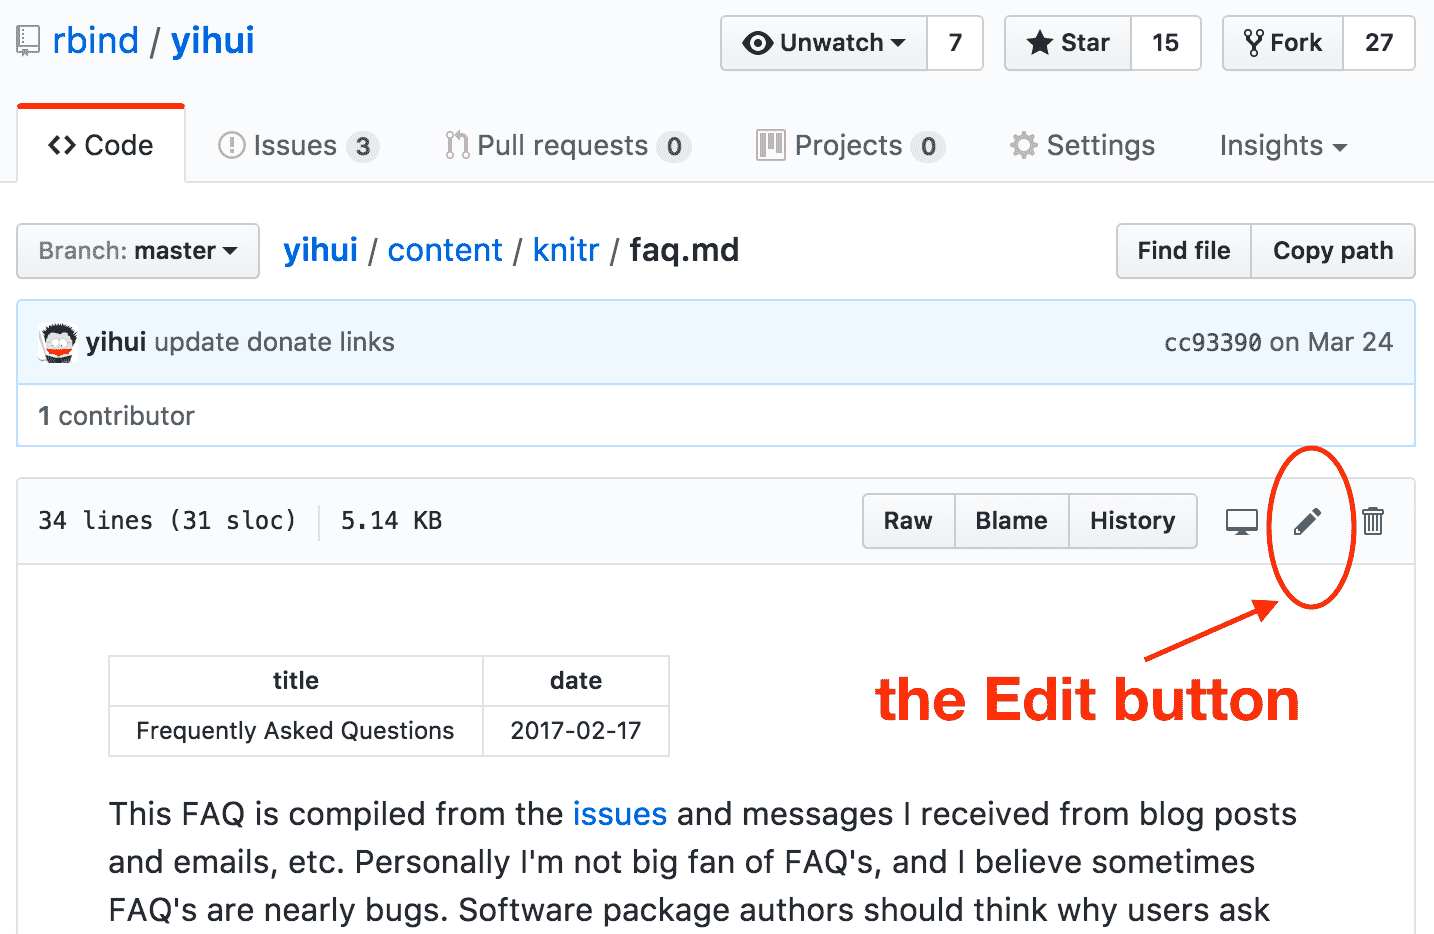
\includegraphics[width=1\linewidth]{images/github-edit} 

}

\caption{Editar un archivo de texto en línea en GitHub.}\label{fig:github-edit}
\end{figure}

Después de digerir el tema XMin y las implementaciones de funciones
adicionales, debería ser mucho más fácil entender las plantillas de
otras personas. Hay una gran cantidad de temas de Hugo, pero las
principales diferencias entre ellos suelen ser estilos. Los componentes
básicos de las plantillas son a menudo similares.

\hypertarget{layouts-personalizados}{%
\section{Layouts personalizados}\label{layouts-personalizados}}

Es muy probable que desee personalizar un tema a menos que lo haya
diseñado. La forma más directa es simplemente hacer cambios directamente
en el tema,\footnote{Si es nuevo en el desarrollo web, tenga cuidado de
  cambiar el contenido dentro del tema. Pequeños cambios como colores y
  tamaños de fuente se pueden encontrar dentro de los archivos CSS del
  tema y pueden modificarse simplemente con el mínimo riesgo de romper
  la funcionalidad del tema.} Pero el problema es que un tema de Hugo
puede ser actualizado constantemente por su autor original para mejoras
o correcciones de errores. De manera similar a la política ``la rompes,
la compras'' (la
\href{https://en.wikipedia.org/wiki/Pottery_Barn_rule}{regla de Pottery
Barn}), una vez que toca el código fuente de otra persona, será
responsable de su mantenimiento futuro, y el autor original no debería
ser responsable de los cambios que haya realizado de su lado. Eso
significa que puede no ser fácil extraer actualizaciones futuras de este
tema a su sitio web (debe leer cuidadosamente los cambios y asegurarse
de que no entren en conflicto con sus cambios), pero si está
completamente satisfecho con el estado actual del tema y no quiere
actualizaciones futuras, está bien modificar los archivos de tema
directamente.

Un autor de tema que tenga en cuenta el hecho de que los usuarios pueden
personalizar su tema generalmente proporcionará dos maneras: una es
proporcionar opciones en \texttt{config.toml}, para que pueda cambiar
estas opciones sin tocar los archivos de la plantilla; la otra es dejar
unos pocos archivos de plantilla livianos en `layouts/' en el tema, para
que pueda anularlos sin tocar los archivos de la plantilla principal.
Tome el tema XMin por ejemplo:

Tengo dos archivos HTML vacíos \texttt{head\_custom.html} y
\texttt{foot\_custom.html} en \texttt{layouts/partials/} en el tema. El
primero se agregará dentro de
\texttt{\textless{}head\textgreater{}\ \textless{}/head\textgreater{}}
de una página, por ejemplo, puede cargar librerías de JavaScript o
incluir hojas de estilo CSS mediante
\texttt{\textless{}link\textgreater{}}. Este último se agregará antes
del pie de página de una página, por ejemplo, puede cargar librerías de
JavaScript adicionales o incrustar comentarios de Disqus allí.

La forma en que personaliza estos dos archivos no es para editarlos
directamente en la carpeta de temas, sino para crear un directorio
\texttt{layouts/partials/} en el directorio raíz de su sitio web, por
ejemplo, su estructura de directorios puede verse así:

\begin{Shaded}
\begin{Highlighting}[]
\ExtensionTok{your-website/}
\NormalTok{├── }\ExtensionTok{config.toml}
\NormalTok{├── }\ExtensionTok{...}
\NormalTok{├── }\ExtensionTok{themes/}
\NormalTok{│   └── }\ExtensionTok{hugo-xmin/}
\NormalTok{│       ├── }\ExtensionTok{...}
\NormalTok{│       └── }\ExtensionTok{layouts/}
\NormalTok{│           ├── }\ExtensionTok{...}
\NormalTok{│           └── }\ExtensionTok{partials}
\NormalTok{│               ├── }\ExtensionTok{foot_custom.html}
\NormalTok{│               ├── }\ExtensionTok{footer.html}
\NormalTok{│               ├── }\ExtensionTok{head_custom.html}
\NormalTok{│               └── }\ExtensionTok{header.html}
\NormalTok{└── }\ExtensionTok{layouts}
\NormalTok{    └── }\ExtensionTok{partials}
\NormalTok{        ├── }\ExtensionTok{foot_custom.html}
\NormalTok{        └── }\ExtensionTok{head_custom.html}
\end{Highlighting}
\end{Shaded}

Todos los archivos en \texttt{layouts/} en el directorio raíz anularán
los archivos con las mismas rutas relativas en
\texttt{themes/hugo-xmin/layouts/}, por ejemplo, el archivo
\texttt{layouts/partials/foot\_custom.html}, cuando se proporcione,
anulará \texttt{themes/hugo-xmin/layouts/partials/foot\_custom.html}.
Eso significa que solo necesita crear y mantener como máximo dos
archivos en \texttt{layouts/} en lugar de mantener todos los archivos
bajo \texttt{themes/}. Tenga en cuenta que este mecanismo de anulación
se aplica a todos los archivos en \texttt{layouts/}, y no está limitado
al directorio \texttt{parials/}. También se aplica a cualquier tema de
Hugo que utilice realmente para su sitio web, y no se limita a
\texttt{hugo-xmin}.

\hypertarget{archivos-estaticos}{%
\section{Archivos estáticos}\label{archivos-estaticos}}

Todos los archivos bajo el directorio
\texttt{static/}\index{Directorio Static} se copian a \texttt{public/}
cuando Hugo procesa un sitio web. Este directorio se usa a menudo para
almacenar archivos web estáticos como imágenes, CSS y archivos de
JavaScript. Por ejemplo, una imagen \texttt{static/foo/bar.png} se puede
incrustar en su publicación usando la sintaxis Markdown
\texttt{!{[}{]}(/foo/bar.png)}.\footnote{El enlace de la imagen depende
  de su configuración \texttt{baseurl} en \texttt{config.toml}. Si no
  contiene un subtrayecto, \texttt{/foo/bar.png} será el enlace de la
  imagen; de lo contrario, tendrá que ajustarlo, por ejemplo, para
  \texttt{baseurl\ =\ "http://example.com/subpath/"}, el enlace a la
  imagen debe ser \texttt{/subpath/foo/bar.png}.}

Por lo general, un tema tiene una carpeta \texttt{static/}, y puede
anular parcialmente sus archivos utilizando el mismo mecanismo que
reemplaza a los \texttt{layouts/} archivos, es decir,
\texttt{static/file} anulará \texttt{themes/theme-name/static/file} . En
el tema XMin, tengo dos archivos CSS \texttt{style.css} y
\texttt{fonts.css}. El primero es la hoja de estilo principal, y el
último es un archivo bastante pequeño para definir tipos de letra
solamente. Es posible que desee definir sus propios tipos de letra, y
solo puede proporcionar un \texttt{static/css/fonts.css} para anular el
del tema, por ejemplo,

\begin{Shaded}
\begin{Highlighting}[]
\NormalTok{body \{}
  \KeywordTok{font-family}\NormalTok{: }\StringTok{"Comic Sans MS"}\NormalTok{, }\DecValTok{cursive}\NormalTok{, }\DecValTok{sans-serif}\NormalTok{;}
\NormalTok{\}}
\NormalTok{code \{}
  \KeywordTok{font-family}\NormalTok{: }\StringTok{"Courier New"}\NormalTok{, Courier, }\DecValTok{monospace}\NormalTok{;}
\NormalTok{\}}
\end{Highlighting}
\end{Shaded}

Para los usuarios de R Markdown, otra aplicación importante del
directorio \texttt{static/} es construir documentos Rmd con formatos de
salida personalizados, es decir, documentos Rmd que no utilizan el
formato \texttt{blogdown::html\_page()} (ver sección
\ref{formatos-de-salida}). Por ejemplo, puede generar un PDF o
presentaciones de documentos Rmd en este directorio, para que Hugo no
los postprocesa, sino que simplemente los copie en \texttt{public/} para
su publicación. Para compilar estos archivos Rmd, debe proporcionar un
script de compilación personalizado \texttt{R/build.R} (consulte la
sección \ref{métodos}). Puede escribir una sola línea de código en este
script\index{blogdown::build\_dir()}:

\begin{Shaded}
\begin{Highlighting}[]
\NormalTok{blogdown}\OperatorTok{::}\KeywordTok{build_dir}\NormalTok{(}\StringTok{"static"}\NormalTok{)}
\end{Highlighting}
\end{Shaded}

La función \texttt{build\_dir()} busca todos los archivos Rmd bajo un
directorio y llama a \texttt{rmarkdown::render()} para compilarlos en
los formatos de salida especificados en los metadatos YAML de los
archivos Rmd. Si sus archivos Rmd no se deben presentar con una simple
llamada \texttt{rmarkdown::render()}, puede proporcionar su propio
código para presentarlos en \texttt{R/build.R}. Hay un mecanismo de
caché integrado en la función \texttt{dir\_desarrollo()}: un archivo Rmd
no se compilará si es anterior a su archivo(s) de salida. Si no desea
este comportamiento, puede obligar a todos los archivos Rmd a volver a
compilarse cada vez: \texttt{build\_dir(force\ =\ TRUE)}.

He proporcionado un ejemplo mínimo en el repositorio de GitHub
\href{https://github.com/yihui/blogdown-static}{yihui/blogdown-static,}
donde puede encontrar dos ejemplos de Rmd en el directorio
\texttt{static/}. Una es una presentación HTML5 basada en el paquete
\textbf{xaringan}, y la otra es un documento PDF basado en
\textbf{bookdown}.

Debe tener precaución con los archivos arbitrarios en \texttt{static/},
debido al mecanismo predominante de Hugo. Es decir, todo en
\texttt{static/} se copiará en \texttt{public/}. Debe asegurarse de que
los archivos que procesa en \texttt{static/} no entrarán en conflicto
con los archivos generados automáticamente por Hugo a partir de
\texttt{content/}. Por ejemplo, si tiene un archivo fuente
\texttt{content/about.md} y un archivo Rmd
\texttt{static/about/index.Rmd} al mismo tiempo, el resultado HTML de
este último sobrescribirá el anterior (tanto Hugo como usted generarán
un archivo de salida con el mismo nombre
\texttt{public/about/index.html}).

\hypertarget{implementacion}{%
\chapter{Implementación}\label{implementacion}}

Dado que el sitio web es básicamente una carpeta que contiene archivos
estáticos, es mucho más fácil de implementar que los sitios web que
requieren lenguajes dinámicos en el servidor, como PHP o bases de datos.
Todo lo que necesita es subir los archivos a un servidor, y generalmente
su sitio web estará en funcionamiento en breve. La pregunta clave es qué
servidor web quiere usar. Si no tiene su propio servidor, puede probar
los que figuran en este capítulo. La mayoría de ellos son gratuitos
(excepto Amazon S3), o al menos ofrecen planes gratuitos. Descargo de
responsabilidad: los autores de este libro no están afiliados a ninguno
de estos servicios o compañías, y no hay garantía de que estos servicios
se presten para siempre.\footnote{Puede encontrar fácilmente otros
  servicios similares si usa su motor de búsqueda}.

Teniendo en cuenta el costo y la amabilidad de los principiantes,
actualmente recomendamos Netlify (\url{https://www.netlify.com}).
Proporciona un plan gratuito que en realidad tiene muchas funciones
útiles. Si no tiene experiencia en publicar sitios web antes, solo
inicie sesión con su cuenta GitHub u otras cuentas, arrastre la carpeta
\texttt{public/} creada por \textbf{blogdown} para su sitio web a la
página de Netlify, y su sitio web estará en línea en unos segundos con
un nombre de subdominio aleatorio del formulario
\texttt{random-word-12345.netlify.com} proporcionado por Netlify (puede
personalizar el nombre). Puede automatizar fácilmente este proceso
(consulte la sección \ref{netlify} para obtener más información). Ya no
necesita luchar con \texttt{ssh} o \texttt{rsync-zrvce}, si sabe lo que
significan estos comandos.

La segunda solución más fácil puede ser Updog (\url{https://updog.co}),
que cuenta con la integración de Dropbox. Publicar un sitio web puede
ser tan fácil como copiar los archivos en la carpeta \texttt{public/} de
su sitio web \textbf{blogdown} en una carpeta de Dropbox. El plan
gratuito de Updog solo ofrece funciones limitadas, y su plan de pago le
dará acceso a funciones mucho más ricas.

Si no le importa utilizar herramientas de línea de comandos o está
familiarizado con GIT/GitHub, puede considerar servicios como GitHub
Pages, Travis CI o Amazon S3 para construir o alojar sus sitios web. No
importa qué servicio use, tenga en cuenta que ninguno de ellos realmente
puede encerrarlo y siempre puede cambiar el servicio. Como mencionamos
anteriormente, una gran ventaja de \textbf{blogdown} es que su sitio web
será una carpeta de archivos estáticos que puede mover a cualquier
servidor web.

\hypertarget{netlify}{%
\section{Netlify}\label{netlify}}

Como acabamos de mencionar, Netlify\index{Netlify} le permite publicar
rápidamente un sitio web cargando la carpeta \texttt{public/} a través
de su interfaz web, y se le asignará un subdominio aleatorio
\texttt{*.netlify.com}.\footnote{Usted no tiene que mantener el dominio
  \texttt{*.netlify.com}. Consulte el apéndice @ref(nombre de dominio)
  para obtener más información.} Este enfoque es bueno para los sitios
web que no se actualizan con frecuencia (o no se actualizan). Sin
embargo, es poco probable que no necesite actualizar su sitio web, por
lo que presentamos un mejor enfoque en esta sección,\footnote{Tenga en
  cuenta que el propósito de esta sección es describir los pasos básicos
  de la publicación de un sitio web con Netlify, y los detalles técnicos
  pueden cambiar de vez en cuando, por lo que la documentación oficial
  de Netlify debería ser la fuente más confiable si tiene alguna
  pregunta o si alguna de las cosas que presentamos aquí no funciona}.
Le llevará unos minutos más completar las configuraciones. Una vez que
está configurado correctamente, todo lo que necesita hacer en el futuro
es actualizar el repositorio fuente, y Netlify llamará a Hugo para que
haga su sitio web automáticamente.

Básicamente, debe alojar todos los archivos fuente de su sitio web en un
repositorio GIT.\footnote{Si el contenido de su sitio \texttt{blogdown}
  no está en el directorio raíz de su repositorio GIT, Netlify no se
  compilará.} No necesita poner el directorio \texttt{public/} bajo
control de versión\footnote{Puede agregar \texttt{public} a
  \texttt{.gitignore} para ignorarlo en GIT.} porque se generará
automáticamente. Actualmente, Netlify admite repositorios GIT alojados
en GitHub, GitLab y BitBucket. Con cualquiera de estas cuentas, puede
iniciar sesión en Netlify desde su página de inicio y seguir la guía
para crear un nuevo sitio desde su repositorio de GIT.

Netlify es compatible con varios generadores de sitios web estáticos,
incluidos Jekyll y Hugo. Para un nuevo sitio, debe especificar un
comando para construir su sitio web, así como también la ruta del
directorio de publicación. Netlify también admite múltiples versiones de
Hugo, por lo que el comando de compilación puede ser el \texttt{hugo}
predeterminado. La versión predeterminada es 0.17, que es demasiado
antigua. Le recomendamos que utilice al menos la versión 0.20. Para
especificar una versión de Hugo mayor o igual a 0.20, debe crear una
variable de entorno \texttt{HUGO\_VERSION} en Netlify. Consulte la
\href{https://www.netlify.com/docs/continuous-deployment/}{documentación
de Netlify} para obtener más información. El directorio de publicación
debe ser \texttt{public} a menos que lo haya cambiado en su
\texttt{config.toml}. La figura @ref(fig: configuración-netlify) muestra
la configuración del sitio web \url{https://t.yihui.name}. No tiene que
seguir la configuración exacta para su propio sitio web; en particular,
es posible que necesite cambiar el valor de la variable de entorno
\texttt{HUGO\_VERSION} a una versión reciente de Hugo.\footnote{Para el
  momento en que se publique este libro, la versión 0.24.1 puede ser
  demasiado antigua.}

\begin{figure}

{\centering 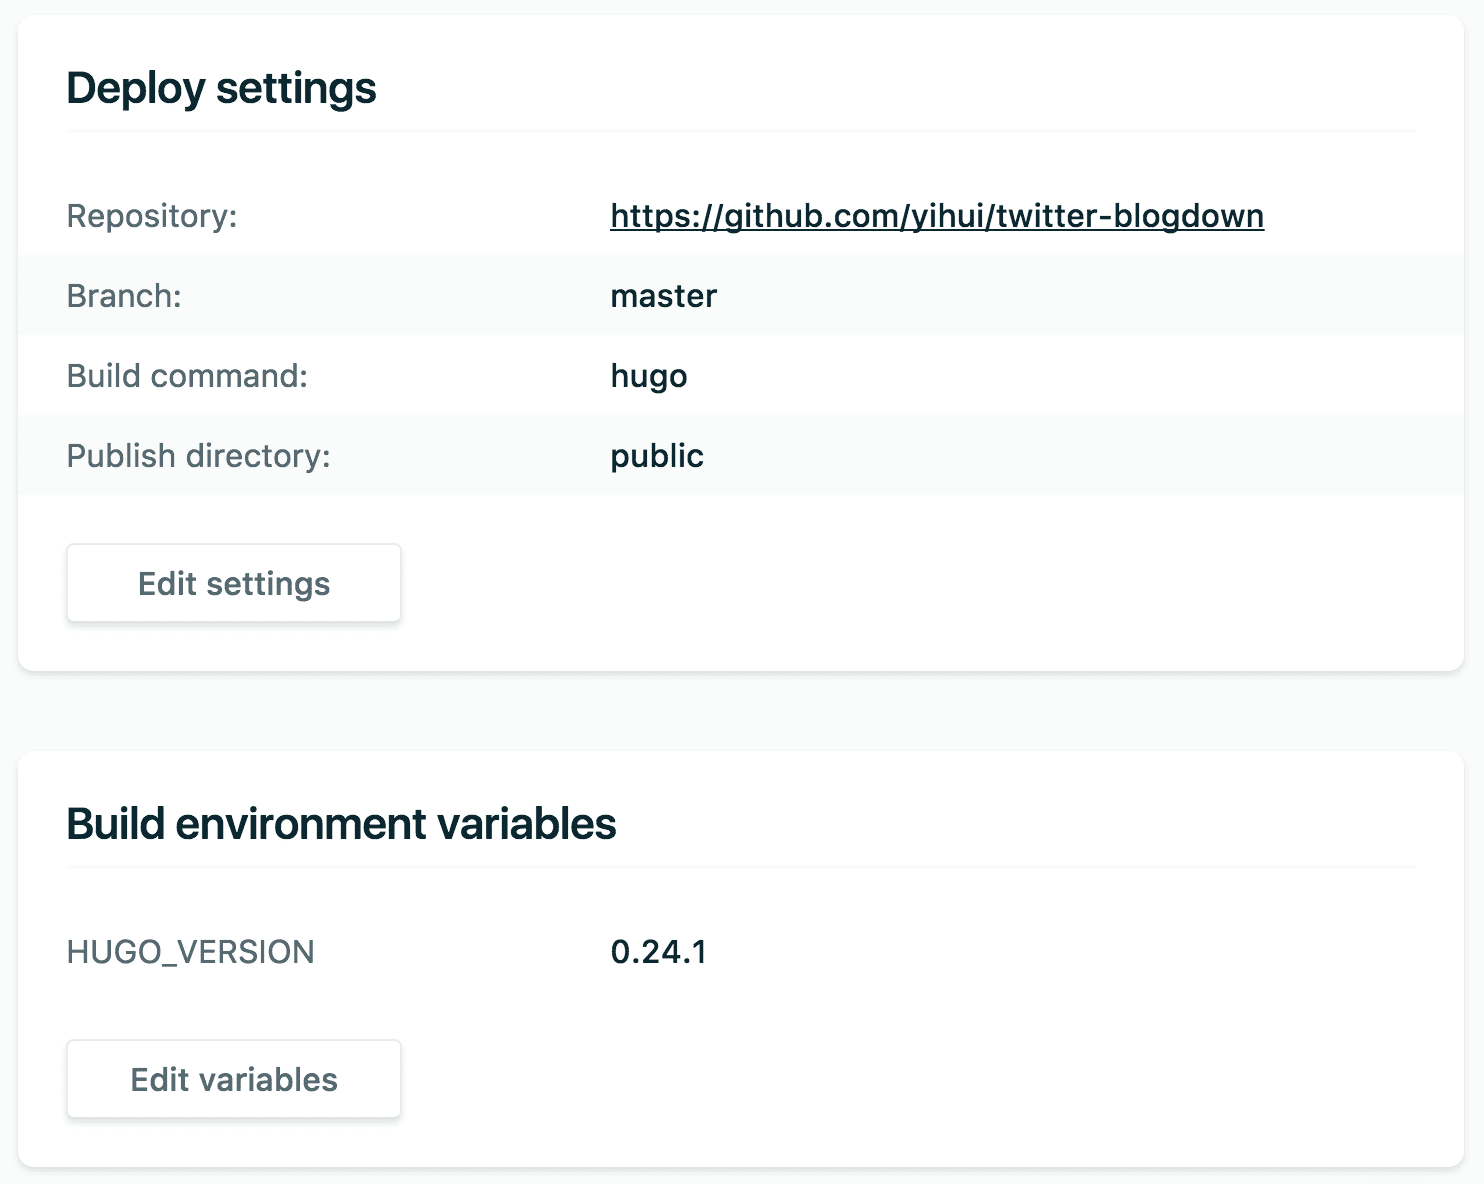
\includegraphics[width=1\linewidth]{images/netlify-settings} 

}

\caption{Configuraciones de ejemplo de un sitio web presentado en Netlify.}\label{fig:netlify-settings}
\end{figure}

Puede tardar uno o dos minutos en implementar su sitio web en Netlify
por primera vez, pero puede ser mucho más rápido más adelante (unos
segundos) cuando actualice el origen de su sitio web, porque Netlify
implementa cambios incrementales en el directorio \texttt{public/}, es
decir, solo se despliegan los archivos más nuevos en comparación con la
última vez.

Después de que su repositorio de GIT esté conectado con Netlify, el
último problema que puede querer resolver es el nombre de
dominio\index{nombre de dominio}, a menos que esté satisfecho con el
subdominio gratuito de Netlify. Si desea utilizar un dominio diferente,
debe configurar algunos registros DNS del dominio para dirigirlo al
servidor de Netlify. Consulte el apéndice @ref(nombre de dominio) para
obtener información general sobre los nombres de dominio.

Si no está familiarizado con los nombres de dominio o no quiere aprender
más sobre ellos, debe tener en cuenta un subdominio gratuito
\texttt{*\ .rbind.io} ofrecido por RStudio, Inc.~Visite el sitio web de
soporte de Rbind \url{https://support.rbind.io} para aprender cómo
solicitar un subdominio. De hecho, la organización Rbind también ofrece
ayuda gratuita sobre cómo configurar un sitio web basado en
\textbf{blogdown}, gracias a una gran cantidad de voluntarios de la
comunidad de R y de estadística.

Netlify es la única solución en este capítulo que no requiere
preinstalar su sitio web. Solo necesita actualizar los archivos fuente,
enviarlos a GitHub y Netlify creará el sitio web para usted.\footnote{Esto
  se denomina ``implementación continua''}. El resto de las soluciones
de este capítulo requerirán que cree su sitio web localmente. y cargue
la carpeta \texttt{public/} explícita o implícitamente. Dicho esto,
ciertamente puede preconstruir su sitio web utilizando cualquier
herramienta, enviarlo a GitHub, y aún así Netlify lo implementará para
usted. Lo que debe hacer es dejar el comando de compilación en blanco y
decirle a Netlify su directorio de publicación (por ejemplo,
\texttt{public/} por defecto de Hugo, pero si su sitio web preconstruido
está bajo el directorio raíz, especifique \texttt{.} como el directorio
de publicación). Entonces Netlify simplemente carga todos los archivos
de este directorio a sus servidores sin reconstruir su sitio web.

\hypertarget{updog}{%
\section{Updog}\label{updog}}

Updog (\url{https://updog.co}) proporciona\index{Updog} un servicio
simple: convierte una carpeta de Dropbox (o Google Drive) especificada
en un sitio web. La idea es que le conceda a Updog el permiso para leer
la carpeta, y actuará como intermediario para mostrar sus archivos en
esta carpeta a sus visitantes. Se debe acceder a esta carpeta a través
de un nombre de dominio, y Updog ofrece un subdominio gratuito
\texttt{*.updog.co}. Por ejemplo, si ha asignado el dominio
\texttt{example.updog.co} a su carpeta de Dropbox, y un visitante desea
ver la página \texttt{https://example.updog.co/foo/index.html}, Updog
leerá el archivo \texttt{foo/index.html} en su carpeta de Dropbox y lo
mostrará al visitante.

Por el momento, el plan gratuito de Updog solo permite un sitio web por
cuenta e insertará un pie de página ``Hosted on Updog'' en sus páginas
web. Puede que no le gusten estas limitaciones. La principal ventaja de
usar Updog es que la publicación de un sitio web se vuelve implícita, ya
que Dropbox sincronizará archivos continuamente. Todo lo que necesita
hacer es asegurarse de que su sitio web se genere en la carpeta correcta
de Dropbox. Esto se puede lograr fácilmente estableciendo la opción
\texttt{publishDir} en \texttt{config.toml}. Por ejemplo, supongamos que
la carpeta que asigna a Updog es
\texttt{\textasciitilde{}/Dropbox/Apps/updog/my-website/}, y su carpeta
fuente está en \texttt{\textasciitilde{}/Dropbox/Apps/updog/my-source/},
entonces puede establecer \texttt{publishDir:\ "../my-website"} en
\texttt{\textasciitilde{}/Dropbox/Apps/updog/my-source/config.toml}.

También puede usar su nombre de dominio personalizado si no desea el
subdominio Updog predeterminado, y solo necesita apuntar el registro
CNAME de su nombre de dominio al subdominio Updog.\footnote{Vea el
  apéndice @ref(nombre de dominio) para obtener más información.}

\hypertarget{github-pages}{%
\section{GitHub Pages}\label{github-pages}}

GitHub Pages (\url{https://pages.github.com}) \index{GitHub Pages} es
una forma muy popular de alojar sitios web estáticos (especialmente los
creados con Jekyll), pero sus ventajas no son obvias ni atractivas en
comparación con Netlify. Le recomendamos que considere Netlify + Hugo
debido a estas razones:

\begin{itemize}
\item
  Actualmente, GitHub Pages no es compatible con HTTPS para nombres de
  dominio personalizados. HTTPS solo funciona para los subdominios
  \texttt{*.github.io}. Esta limitación no existe en Netlify. Puede leer
  el artículo \href{https://https.cio.gov/everything/}{``¿Por qué HTTPS
  para todo?''} para comprender por qué es importante y se le anima a
  activar HTTPS para su sitio web siempre que sea posible.
\item
  Redirigir URLs es incómodo con GitHub Pages pero mucho más sencillo
  con Netlify.\footnote{GitHub Pages utiliza un plugin Jekyll para
    escribir una metaetiqueta \texttt{HTTP-REFRESH} para redirigir
    páginas, y Netlify puede hacer redirecciones 301 o 302 basadas en
    patrones, que puede notificar a los motores de búsqueda que ciertas
    páginas se han movido (de forma permanente o temporal).} Esto es
  importante especialmente cuando tiene un sitio web antiguo que desea
  migrar a Hugo; algunos enlaces pueden estar rotos, en cuyo caso puede
  redireccionarlos fácilmente con Netlify.
\item
  Una de las mejores características de Netlify que no está disponible
  en GitHub Pages es que Netlify puede generar un sitio web único para
  la vista previa cuando se envía un pull request de GitHub a su
  repositorio de GitHub. Esto es extremadamente útil cuando otra persona
  (o incluso usted mismo) propone cambios en su sitio web, ya que tiene
  la oportunidad de ver cómo se vería el sitio web antes de fusionar el
  pull request.
\end{itemize}

Básicamente, Netlify puede hacer todo lo que GitHub Pages puede, pero
todavía hay una pequeña característica que falta, que está estrechamente
vinculada a GitHub, que es GitHub
\href{https://help.github.com/articles/user-organization-and-project-pages/}{Project
Pages.}. Esta función le permite tener sitios web de proyectos en
repositorios separados, por ejemplo, puede tener dos sitios web
independientes \texttt{https://username.github.io/proj-a/} y
\texttt{https://username.github.io/proj-b/}, que corresponde a los
repositorios de GitHub \texttt{username/proj-a} y
\texttt{username/proj-b}, respectivamente. Sin embargo, dado que puede
conectar cualquier repositorio de GitHub con Netlify, y cada repositorio
puede asociarse con un nombre de dominio o subdominio, puede reemplazar
las páginas de proyecto de GitHub con diferentes subdominios como
\texttt{proj-a.netlify.com} y \texttt{proj-b.netlify.com}. La limitación
real es que no puede usar subcampos en la URL pero puede usar cualquier
(sub)nombre de dominio.

Aunque GitHub no es compatible oficialmente con Hugo (solo es compatible
con Jekyll), puede publicar cualquier archivo HTML estático en GitHub
Pages, incluso si no están compiladas con Jekyll. El primer requisito
para usar GitHub Pages es que debe crear un repositorio de GitHub
llamado \texttt{username.github.io} debajo de su cuenta (reemplace
\texttt{username} con su nombre de usuario GitHub real), y lo que queda
es llevar los archivos de su sitio web a este repositorio. La
documentación completa de GitHub Pages está en
\url{https://pages.github.com}, y por favor ignore todo lo relacionado
con Jekyll a menos que realmente use Jekyll en lugar de Hugo. Para
asegurarse de que GitHub no reconstruya su sitio web utilizando Jekyll y
simplemente publique los archivos que envía al repositorio, debe crear
un archivo (oculto) llamado \texttt{.nojekyll} en el
repositorio.\footnote{Puede usar la función en R
  \texttt{file.create(\textquotesingle{}.nojekyll\textquotesingle{})}
  para crear este archivo si no sabe cómo hacerlo.} GitHub ofrece un
subdominio gratuito \texttt{username.github.io}, y puede usar su propio
nombre de dominio configurando sus registros A o CNAME para apuntarlo a
GitHub Pages (consulte la documentación de GitHub Pages para obtener
instrucciones).

Su directorio \texttt{public/} debe ser el repositorio de GIT. Tienes
dos opciones posibles para configurar este repositorio localmente. La
primera opción es seguir la estructura predeterminada de un sitio web de
Hugo como el siguiente diagrama e inicializar el repositorio de GIT bajo
el directorio \texttt{public/}:

\begin{Shaded}
\begin{Highlighting}[]
\ExtensionTok{source/}
\NormalTok{│}
\NormalTok{├── }\ExtensionTok{config.toml}
\NormalTok{├── }\ExtensionTok{content/}
\NormalTok{├── }\ExtensionTok{themes/}
\NormalTok{├── }\ExtensionTok{...}
\NormalTok{└── }\ExtensionTok{public/}
    \KeywordTok{|}
\NormalTok{    ├── }\ExtensionTok{.git/}
\NormalTok{    ├── }\ExtensionTok{.nojekyll}
\NormalTok{    ├── }\ExtensionTok{index.html}
\NormalTok{    ├── }\ExtensionTok{about/}
\NormalTok{    └── }\ExtensionTok{...}
\end{Highlighting}
\end{Shaded}

Si sabe cómo usar la línea de comandos, cambie el directorio de trabajo
a \texttt{public/}, e inicialice el repositorio de GIT allí:

\begin{Shaded}
\begin{Highlighting}[]
\BuiltInTok{cd}\NormalTok{ public}
\FunctionTok{git}\NormalTok{ init}
\FunctionTok{git}\NormalTok{ remote add origin https://github.com/username/username.github.io}
\end{Highlighting}
\end{Shaded}

La otra opción es clonar el repositorio de GitHub que creó en el mismo
directorio que el origen de su sitio web:

\begin{Shaded}
\begin{Highlighting}[]
\FunctionTok{git}\NormalTok{ clone https://github.com/username/username.github.io}
\end{Highlighting}
\end{Shaded}

Y la estructura debería lucir más o menos así:

\begin{Shaded}
\begin{Highlighting}[]
\ExtensionTok{source/}
\NormalTok{│}
\NormalTok{├── }\ExtensionTok{config.toml}
\NormalTok{├── }\ExtensionTok{content/}
\NormalTok{├── }\ExtensionTok{themes/}
\NormalTok{└── }\ExtensionTok{...}

\ExtensionTok{username.github.io/}
\NormalTok{│}
\NormalTok{├── }\ExtensionTok{.git/}
\NormalTok{├── }\ExtensionTok{.nojekyll}
\NormalTok{├── }\ExtensionTok{index.html}
\NormalTok{├── }\ExtensionTok{about/}
\NormalTok{└── }\ExtensionTok{...}
\end{Highlighting}
\end{Shaded}

El directorio de origen y el directorio \texttt{username.github.io}
están bajo el mismo directorio principal. En este caso, debe establecer
la opción \texttt{publishDir:\ "../username.github.io"} en
\texttt{source/config.toml}.

\hypertarget{travis-github}{%
\section{Travis + GitHub}\label{travis-github}}

Si\index{Travis CI} decide no seguir nuestra recomendación de usar
Netlify para implementar su sitio web, debemos advertirle que el enfoque
de esta sección requerirá un conocimiento sustancial sobre GIT, GitHub,
Travis CI (\url{https://travis-ci.org}), y la línea de comandos de
Linux, que dejaremos que aprenda por su cuenta. La principal ventaja de
publicar a través de Travis CI es que puede compilar todas sus
publicaciones de Rmd en Travis CI (en la nube) en lugar de su
computadora local.

En caso de que no esté familiarizado con Travis, este es un servicio de
verificación continua de su software en una máquina virtual cada vez que
haga push a cambios en GitHub. Es principalmente para probar software,
pero dado que puede ejecutar muchos comandos en su máquina virtual,
puede usar la máquina virtual para hacer otras cosas, por ejemplo,
instalar R y el paquete \textbf{blogdown} para crear sitios web. Antes
de mostrarle cómo, me gustaría mencionar dos cuestiones que debe tener
en cuenta:

\begin{itemize}
\item
  Personalmente, prefiero echar un vistazo a la salida en GIT para ver
  los cambios cuando tengo cualquier salida que se calcula dinámicamente
  desde R, para que sepa con certeza qué voy a publicar exactamente. Con
  Travis, es algo impredecible porque es completamente automático y no
  tiene la oportunidad de ver el nuevo contenido o los resultados que se
  publicarán. Hay muchos factores que pueden afectar la construcción del
  sitio: la versión de R, la disponibilidad de ciertos paquetes en R,
  las dependencias del sistema y la conexión de red, etc.
\item
  El tiempo requerido para compilar todos los archivos Rmd puede ser muy
  largo y causar tiempos de espera en Travis, dependiendo de cuánto
  tiempo consuma su código en R. Hay un mecanismo de almacenamiento en
  caché en \textbf{blogdown} para acelerar la construcción de su sitio
  (consulte la sección \ref{métodos}), y si usa Travis para construir su
  sitio web, no se beneficiará de este mecanismo de almacenamiento en
  caché a menos que aproveche el almacenamiento en caché de Travis.
  Tiene que almacenar en caché los directorios \texttt{content/},
  \texttt{static/}, y \texttt{blogdown/}, pero el caché de Travis es un
  poco frágil, en mi experiencia. Algunas veces la memoria caché puede
  ser purgada por razones desconocidas. Además, no puede almacenar en
  caché directamente \texttt{content/} y \texttt{static/}, porque Travis
  clona su repositorio antes de restaurar el caché, lo que significa que
  los archivos viejos del \texttt{content/} y \texttt{static/}
  almacenados en caché pueden sobrescribir los nuevos archivos que usted
  envió a GitHub.
\end{itemize}

El segundo problema se puede resolver, pero no quiero explicar cómo en
este libro, ya que la solución es demasiado complicada. Si realmente
desea usar Travis para construir su sitio web y encontrarse con este
problema, puede presentar un issue en el repositorio de GitHub
\url{https://github.com/yihui/travis-blogdown}. De hecho, este
repositorio es un ejemplo mínimo que creé para mostrar cómo crear un
sitio web en Travis y publicarlo en GitHub Pages.

La documentación de Travis muestra cómo implementar un sitio en GitHub
Pages: \url{https://docs.travis-ci.com/user/deployment/pages/}, pero no
muestra cómo crear un sitio. Aquí está el archivo de configuración de
Travis, \texttt{.travis.yml}, para el repositorio
\texttt{travis-blogdown}:

\begin{Shaded}
\begin{Highlighting}[]
\FunctionTok{language:}\AttributeTok{ r}
\FunctionTok{dist:}\AttributeTok{ trusty}
\FunctionTok{sudo:}\AttributeTok{ false}

\FunctionTok{branches:}
  \FunctionTok{only:}
    \KeywordTok{-}\NormalTok{ master}

\FunctionTok{cache:}
  \FunctionTok{packages:}\AttributeTok{ yes}
  \FunctionTok{directories:}
    \KeywordTok{-}\NormalTok{ $HOME/bin}

\FunctionTok{before_script:}
  \KeywordTok{-} \StringTok{"Rscript -e 'blogdown::install_hugo()'"}

\FunctionTok{script:}
  \KeywordTok{-} \StringTok{"Rscript -e 'blogdown::build_site()'"}

\FunctionTok{deploy:}
  \FunctionTok{provider:}\AttributeTok{ pages}
  \FunctionTok{skip_cleanup:}\AttributeTok{ true}
  \FunctionTok{github_token:}\AttributeTok{ $GITHUB_TOKEN}
  \FunctionTok{on:}
    \FunctionTok{branch:}\AttributeTok{ master}
  \FunctionTok{local_dir:}\AttributeTok{ public}
  \FunctionTok{fqdn:}\AttributeTok{ travis-blogdown.yihui.name}
\end{Highlighting}
\end{Shaded}

La clave es que instalemos Hugo a través de
\texttt{blogdown::install\_hugo()} y construyamos el sitio a través de
\texttt{blogdown::build\_site()}. Para engañar a Travis para que cree
este repositorio como un paquete en R, debe tener un archivo
\texttt{DESCRIPTION} en el repositorio, de lo contrario, su sitio web no
se compilará.

\begin{Shaded}
\begin{Highlighting}[]
\FunctionTok{Package:}\AttributeTok{ placeholder}
\FunctionTok{Type:}\AttributeTok{ Website}
\FunctionTok{Title:}\AttributeTok{ Does not matter.}
\FunctionTok{Version:}\AttributeTok{ 0.0.1}
\FunctionTok{Imports:}\AttributeTok{ blogdown}
\FunctionTok{Remotes:}\AttributeTok{ rstudio/blogdown}
\end{Highlighting}
\end{Shaded}

Hay algunas cosas más que explicar y enfatizar en \texttt{.travis.yml}:

\begin{itemize}
\item
  La opción \texttt{branches} especifica que solo los cambios en la rama
  \texttt{master} activarán la construcción en Travis.
\item
  La opción \texttt{cache} especifica todos los paquetes en R que se
  almacenarán en caché, por lo que la próxima vez será más rápido crear
  el sitio (no es necesario volver a instalar los paquetes en R desde el
  origen). El directorio \texttt{bin/} en el directorio de inicio
  también se almacena en caché porque Hugo está instalado allí, y la
  próxima vez que Hugo no necesite ser reinstalado.
\item
  Para la opción \texttt{deploy}, hay una variable de entorno llamada
  \texttt{GITHUB\_TOKEN}, y he especificado su valor para ser un token
  de acceso personal de GitHub a través de la configuración de Travis de
  este repositorio, para que Travis pueda escribir en mi repositorio
  después de que el sitio web está construido. La opción \texttt{on}
  especifica que la implementación solo ocurrirá cuando se construya la
  rama \texttt{master}. La opción \texttt{local\_dir} es el directorio
  de publicación, que debe ser `público' por defecto en Hugo. Por
  defecto, el sitio web se envía a la rama \texttt{gh-pages} de este
  repositorio. La opción \texttt{fqdn} especifica el dominio
  personalizado del sitio web. He establecido un registro CNAME (ver
  apéndice @ref(nombre de dominio)) para apuntar
  \texttt{travis-blogdown.yihui.name} a \texttt{yihui.github.io}, para
  que GitHub pueda servir a este sitio web a través de este dominio (de
  hecho, Travis escribirá un archivo \texttt{CNAME} que contiene el
  dominio en la rama \texttt{gh-pages}).
\end{itemize}

Si utiliza el repositorio \texttt{username.github.io} en GitHub, el
sitio web debe ser enviado a su rama \texttt{master} en lugar de
\texttt{gh-pages} (esta es la única excepción). Recomiendo que separe el
repositorio fuente y el repositorio de salida. Por ejemplo, puede tener
un repositorio \texttt{website-source} con la misma configuración que el
\texttt{.travis.yml} anterior, excepto dos nuevas opciones bajo
\texttt{deploy}:

\begin{Shaded}
\begin{Highlighting}[]
\FunctionTok{deploy:}
\NormalTok{  ...}
  \FunctionTok{repo:}\AttributeTok{ username/username.github.io}
  \FunctionTok{target_branch:}\AttributeTok{ master}
\end{Highlighting}
\end{Shaded}

Esto significa que el sitio web será enviado a la rama \texttt{master}
del repositorio \texttt{username/username.github.io} (recuerde
reemplazar \texttt{username} con su nombre de usuario real).

También puede implementar su sitio web en Amazon S3\index{Amazon S3}, y
la configuración desde R es muy similar a lo que hemos introducido para
GitHub Pages. La única diferencia está en el último paso, donde cambia
el destino de GitHub Pages a Amazon S3. Para obtener más información,
consulte la documentación de Travis:
\url{https://docs.travis-ci.com/user/deployment/s3/}.

\hypertarget{gitlab-pages}{%
\section{GitLab Pages}\label{gitlab-pages}}

GitLab (\url{http://gitlab.com}) es una forma muy popular de alojar el
código fuente de su proyecto. GitLab tiene un
\href{https://about.gitlab.com/features/gitlab-ci-cd/}{servicio de
Integración y Despliegue Integrado (CI/CD)} que se puede usar para
alojar sitios web estáticos, llamados
\href{https://about.gitlab.com/features/pages/}{Páginas de GitLab}. La
principal ventaja de utilizar GitLab Pages es que podrá compilar todas
sus publicaciones Rmd a través de su servicio CI/CD en lugar de su
computadora local y cualquier contenido generado, como archivos HTML, se
copiará automáticamente en el servidor web. Tenga en cuenta que este
enfoque tiene problemas similares a los del enfoque Travis + GitHub en
la sección \ref{travis-github}.

El servicio CI/CD de GitLab usa las instrucciones almacenadas en el
archivo YAML \texttt{.gitlab-ci.yml} en el repositorio. Aquí hay un
archivo de configuración de muestra \texttt{.gitlab-ci.yml} del
repositorio de ejemplo \url{https://gitlab.com/rgaiacs/blogdown-gitlab}:

\begin{Shaded}
\begin{Highlighting}[]
\FunctionTok{image:}\AttributeTok{ debian:buster-slim}

\FunctionTok{before_script:}
  \KeywordTok{-}\NormalTok{ apt-get update && apt-get -y install pandoc r-base}
  \KeywordTok{-} \FunctionTok{R -e "install.packages('blogdown',repos='http:}\AttributeTok{//cran.rstudio.com')"}
  \KeywordTok{-} \FunctionTok{R -e "blogdown:}\AttributeTok{:install_hugo()"}

\FunctionTok{pages:}
  \FunctionTok{script:}
    \KeywordTok{-} \FunctionTok{R -e "blogdown:}\AttributeTok{:build_site()"}
  \FunctionTok{artifacts:}
    \FunctionTok{paths:}
      \KeywordTok{-}\NormalTok{ public}
  \FunctionTok{only:}
    \KeywordTok{-}\NormalTok{ master}
\end{Highlighting}
\end{Shaded}

La opción \texttt{image} especifica qué imagen de
\href{https://www.docker.com}{Docker} se usará como punto de inicio.
Estamos utilizando una imagen de Debian, pero se puede usar cualquier
imagen de \href{https://hub.docker.com/}{Docker Hub}. Otras
configuraciones y opciones son similares a \texttt{.travis.yml} en la
sección \ref{travis-github}. El ejemplo anterior genera el sitio web en
\url{https://rgaiacs.gitlab.io/blogdown-gitlab}.

\hypertarget{migration}{%
\chapter{Migration}\label{migration}}

Por lo general, es más fácil iniciar un nuevo sitio web que
migrar\index{Migración del sitio} un antiguo a un nuevo framework, pero
puede que tenga que hacerlo de todos modos debido al contenido útil en
el viejo sitio web que no debe descartarse simplemente. Una solución
perezosa es abandonar el sitio web antiguo tal como está, iniciar un
nuevo sitio web con un nuevo dominio y proporcionar un enlace al sitio
web anterior. Esto puede ser molesto para sus lectores, y es posible que
no puedan descubrir fácilmente las gemas que usted creó en su sitio web
antiguo, por lo que le recomendamos que migre sus publicaciones y
páginas anteriores al nuevo sitio web si es posible.

Este proceso puede ser fácil o difícil, dependiendo de lo complicado que
sea el sitio web anterior. La mala noticia es que no es probable que
haya una solución universal o mágica, pero he proporcionado algunas
funciones de ayuda en \textbf{blogdown} y una aplicación Shiny para
ayudarlo, lo que puede hacer que sea un poco más fácil para usted migrar
de los sitios de Jekyll y WordPress.

Para darle una idea sobre la posible cantidad de trabajo requerido, le
puedo decir que me tomó una semana entera (de la mañana a la medianoche
todos los días) migrar varios de mis sitios web personales basados en
Jekyll a Hugo y \textbf{blogdown}. La complicación en mi caso no era
solo Jekyll, sino también el hecho de que construí varios sitios web de
Jekyll (porque no tenía opción en Jekyll) y quería unirlos en el mismo
repositorio. Ahora mis dos blogs (chino e inglés), la documentación del
paquete \textbf{knitr} \citep{R-knitr} y la documentación del paquete
\textbf{animation} \citep{R-animation} se mantienen en el mismo
repositorio: \url{https://github.com/rbind/yihui}. Tengo alrededor de
1000 páginas en este sitio web, la mayoría de las cuales son
publicaciones de blog. Solía llevarme más de 30 segundos obtener una
vista previa de mi blog en Jekyll, y ahora toma menos de 2 segundos
construir el sitio en Hugo.

Otro ejemplo complicado es el sitio web de Rob J Hyndman
(\url{https://robjhyndman.com}). Comenzó su sitio web en 1993 (12 años
antes que yo), y había acumulado una gran cantidad de contenido a lo
largo de los años. Puede leer la publicación
\url{https://support.rbind.io/2017/05/15/converting-robjhyndman-to-blogdown/}
para las historias sobre cómo migró su sitio web de WordPress a
\textbf{blogdown}. La clave es que probablemente necesite un vuelo
internacional largo cuando desee migrar un sitio web complicado.

Un ejemplo más simple es el blog Simply Statistics
(\url{https://simplystatistics.org}). Originalmente fue construido en
Jekyll\footnote{Fue migrado de WordPress hace unos años. El sitio de
  WordPress en realidad se migró de un blog anterior de Tumblr.} Y la
fuente se alojó en el repositorio de GitHub
\url{https://github.com/simplystats/simplystats.github.io}. Me ofrecí
como voluntario para ayudarlos a pasar a \textbf{blogdown}, y me tomó
aproximadamente cuatro horas. Mi tiempo se gastó principalmente en
limpiar los metadatos YAML de publicaciones y retocar el tema Hugo.
Tenían alrededor de 1000 publicaciones, lo que parece mucho, pero el
número en realidad no importa, porque escribí un guión en R para
procesar todas las publicaciones automáticamente. El nuevo repositorio
está en \url{https://github.com/rbind/simplystats}.

Si realmente no tiene demasiadas páginas (por ejemplo, menos de 20), le
recomiendo que las corte y las pegue en los archivos Markdown, porque en
realidad puede llevar más tiempo escribir un script para procesar estas
páginas.

Es probable que algunos enlaces se rompan después de la migración porque
Hugo genera diferentes enlaces para sus páginas y publicaciones. En ese
caso, puede corregir los enlaces permanentes (por ejemplo, ajustando la
barra de una publicación) o usar 301 redireccionamientos (por ejemplo,
en Netlify).

\hypertarget{desde-jekyll}{%
\section{Desde Jekyll}\label{desde-jekyll}}

Al convertir un sitio web de Jekyll\index{Jekyll} en Hugo, la parte más
desafiante es el tema. Si desea mantener exactamente el mismo tema,
deberá volver a escribir las plantillas de Jekyll utilizando la sintaxis
de Hugo (consulte la sección \ref{templates}). Sin embargo, si puede
encontrar un tema existente en Hugo (\url{https://themes.gohugo.io}),
las cosas serán mucho más fáciles, y usted solo necesita mover el
contenido de su sitio web a Hugo, lo cual es relativamente fácil.
Básicamente, copie las páginas y publicaciones de Markdown en el
directorio \texttt{content/} en Hugo y modifique estos archivos de
texto.

Usualmente, las publicaciones en Jekyll están bajo el directorio
\texttt{\_posts/}, y puedes moverlas a \texttt{content/post/} (puede
usar otros directorios). Luego, debe definir una regla personalizada
para las URL permanentes en \texttt{config.toml} (consulte la sección
\ref{opciones}):

\begin{Shaded}
\begin{Highlighting}[]
\NormalTok{[permalinks]}
\NormalTok{    post }\OperatorTok{=} \StringTok{"/:year/:month/:day/:slug/"}
\end{Highlighting}
\end{Shaded}

Esto depende del formato de las URL que utilizó en Jekyll (consulte la
opción \texttt{permalink} en su \texttt{\_config.yml}).

Si hay archivos estáticos como imágenes, se pueden mover al directorio
\texttt{static/} en Hugo.

Luego necesita usar su herramienta favorita con algunas técnicas de
manipulación de cadenas de caracteres para procesar todos los archivos
Markdown. Si usa R, puede listar todos los archivos Markdown y
procesarlos uno por uno en un bucle. A continuación se muestra un boceto
del código:

\begin{Shaded}
\begin{Highlighting}[]
\NormalTok{files =}\StringTok{ }\KeywordTok{list.files}\NormalTok{(}
  \StringTok{'content/'}\NormalTok{, }\StringTok{'[.](md|markdown)$'}\NormalTok{, }\DataTypeTok{full.names =} \OtherTok{TRUE}\NormalTok{,}
  \DataTypeTok{recursive =} \OtherTok{TRUE}
\NormalTok{)}
\ControlFlowTok{for}\NormalTok{ (f }\ControlFlowTok{in}\NormalTok{ files) \{}
\NormalTok{  blogdown}\OperatorTok{:::}\KeywordTok{process_file}\NormalTok{(f, }\ControlFlowTok{function}\NormalTok{(x) \{}
    \CommentTok{# process x here and return the modified x}
\NormalTok{    x}
\NormalTok{  \})}
\NormalTok{\}}
\end{Highlighting}
\end{Shaded}

La función \texttt{process\_file()} es una función auxiliar interna en
\textbf{blogdown}. Se necesita un nombre de archivo y una función de
procesador para manipular el contenido del archivo y escribe el texto
modificado de nuevo en el archivo.

Para darle una idea de cómo puede ser una función de procesador,
proporcioné algunas funciones simples de ayuda en \textbf{blogdown}, y a
continuación hay dos de ellas:

\begin{Shaded}
\begin{Highlighting}[]
\NormalTok{blogdown}\OperatorTok{:::}\NormalTok{remove_extra_empty_lines}
\end{Highlighting}
\end{Shaded}

\begin{verbatim}
function (f) 
process_file(f, function(x) {
    x = paste(gsub("\\s+$", "", x), collapse = "\n")
    trim_ws(gsub("\n{3,}", "\n\n", x))
})
<environment: namespace:blogdown>
\end{verbatim}

\begin{Shaded}
\begin{Highlighting}[]
\NormalTok{blogdown}\OperatorTok{:::}\NormalTok{process_bare_urls}
\end{Highlighting}
\end{Shaded}

\begin{verbatim}
function (f) 
process_file(f, function(x) {
    gsub("\\[([^]]+)]\\(\\1/?\\)", "<\\1>", x)
})
<environment: namespace:blogdown>
\end{verbatim}

La primera función sustituye dos o más líneas vacías con una sola línea
vacía. La segunda función reemplaza los enlaces de la forma
\texttt{{[}url{]}(url)} con \texttt{\textless{}url\textgreater{}}. Sin
embargo, no hay nada de malo con las líneas vacías excesivas o la
sintaxis \texttt{{[}url{]}(url)}. Estas funciones auxiliares pueden
hacer que su texto de Markdown sea un poco más limpio. Puede encontrar
todas las funciones auxiliares en
\url{https://github.com/rstudio/blogdown/blob/master/R/clean.R}. Tenga
en cuenta que no se exportan de \textbf{blogdown}, por lo que necesita
tres puntos y coma para acceder a ellos.

Es posible que los metadatos YAML de sus publicaciones no estén
completamente limpios, especialmente cuando su sitio web Jekyll se
convirtió de un sitio web anterior de WordPress. La función auxiliar
interna \texttt{blogdown:::modify\_yaml()} puede ayudarlo a limpiar los
metadatos. Por ejemplo, a continuación se muestran los metadatos YAML de
una publicación de blog de Simply Statistics cuando se creó en Jekyll:

\begin{Shaded}
\begin{Highlighting}[]
\OtherTok{---}
\FunctionTok{id:}\AttributeTok{ 4155}
\FunctionTok{title:}\AttributeTok{ Announcing the JHU Data Science Hackathon 2015}
\FunctionTok{date:}\AttributeTok{ 2015-07-28T13:31:04+00:00}
\FunctionTok{author:}\AttributeTok{ Roger Peng}
\FunctionTok{layout:}\AttributeTok{ post}
\FunctionTok{guid:}\AttributeTok{ http://simplystatistics.org/?p=4155}
\FunctionTok{permalink:}\AttributeTok{ /2015/07/28/announcing-the-jhu-data-science-hackathon-2015}
\FunctionTok{pe_theme_meta:}
  \KeywordTok{-} \StringTok{'O:8:"stdClass":2:\{s:7:"gallery";O:8:"stdClass":...\}'}
\FunctionTok{al2fb_facebook_link_id:}
  \KeywordTok{-}\NormalTok{ 136171103105421_837886222933902}
\FunctionTok{al2fb_facebook_link_time:}
  \KeywordTok{-} \FunctionTok{2015-07-28T17:}\AttributeTok{31:11+00:00}
\FunctionTok{al2fb_facebook_link_picture:}
  \KeywordTok{-} \FunctionTok{post=http:}\AttributeTok{//simplystatistics.org/?al2fb_image=1}
\FunctionTok{dsq_thread_id:}
  \KeywordTok{-}\NormalTok{ 3980278933}
\FunctionTok{categories:}
  \KeywordTok{-}\NormalTok{ Uncategorized}
\OtherTok{---}
\end{Highlighting}
\end{Shaded}

Puede descartar los campos YAML que no son útiles en Hugo. Por ejemplo,
solo puede mantener los campos \texttt{title}, \texttt{author},
\texttt{date}, \texttt{categories} y \texttt{tags}, y descartar otros
campos. En realidad, es posible que también desee agregar un campo
\texttt{slug} que tome el nombre de archivo base de la publicación (sin
la fecha inicial). Por ejemplo, cuando el nombre del archivo postal es
\texttt{2015-07-28-announceing-the-jhu-data-science-hackathon-2015.md},
es posible que desee agregar
\texttt{slug:\ announcing-the-jhu-data-science-hackathon-2015} para
asegurarse de que la URL de la publicación en el nuevo sitio siga siendo
la misma.

Aquí está el código para procesar los metadatos YAML de todas las
publicaciones:

\begin{Shaded}
\begin{Highlighting}[]
\ControlFlowTok{for}\NormalTok{ (f }\ControlFlowTok{in}\NormalTok{ files) \{}
\NormalTok{  blogdown}\OperatorTok{:::}\KeywordTok{modify_yaml}\NormalTok{(f, }\DataTypeTok{slug =} \ControlFlowTok{function}\NormalTok{(old, yaml) \{}
    \CommentTok{# YYYY-mm-dd-name.md -> name}
    \KeywordTok{gsub}\NormalTok{(}\StringTok{'^}\CharTok{\textbackslash{}\textbackslash{}}\StringTok{d\{4\}-}\CharTok{\textbackslash{}\textbackslash{}}\StringTok{d\{2\}-}\CharTok{\textbackslash{}\textbackslash{}}\StringTok{d\{2\}-|[.](md|markdown)'}\NormalTok{, }\StringTok{''}\NormalTok{, f)}
\NormalTok{  \}, }\DataTypeTok{categories =} \ControlFlowTok{function}\NormalTok{(old, yaml) \{}
    \CommentTok{# remove the Uncategorized category}
    \KeywordTok{setdiff}\NormalTok{(old, }\StringTok{'Uncategorized'}\NormalTok{)}
\NormalTok{  \}, }\DataTypeTok{.keep_fields =} \KeywordTok{c}\NormalTok{(}
    \StringTok{'title'}\NormalTok{, }\StringTok{'author'}\NormalTok{, }\StringTok{'date'}\NormalTok{, }\StringTok{'categories'}\NormalTok{, }\StringTok{'tags'}\NormalTok{, }\StringTok{'slug'}
\NormalTok{  ), }\DataTypeTok{.keep_empty =} \OtherTok{FALSE}\NormalTok{)}
\NormalTok{\}}
\end{Highlighting}
\end{Shaded}

Puede pasar una ruta de archivo a \texttt{modify\_yaml()}, definir
nuevos valores YAML (o funciones para devolver nuevos valores basados en
los valores anteriores) y decidir qué campos conservar
(\texttt{.keep\_fields}). Puede descartar campos vacíos a través de
\texttt{.keep\_empty\ =\ FALSE}. Los metadatos YAML procesados están a
continuación, lo que parece mucho más limpio:

\begin{Shaded}
\begin{Highlighting}[]
\OtherTok{---}
\FunctionTok{title:}\AttributeTok{ Announcing the JHU Data Science Hackathon 2015}
\FunctionTok{author:}\AttributeTok{ Roger Peng}
\FunctionTok{date:}\AttributeTok{ }\StringTok{'2015-07-28T13:31:04+00:00'}
\FunctionTok{slug:}\AttributeTok{ announcing-the-jhu-data-science-hackathon-2015}
\OtherTok{---}
\end{Highlighting}
\end{Shaded}

\hypertarget{desde-wordpress}{%
\section{Desde WordPress}\label{desde-wordpress}}

Según nuestra experiencia, la mejor manera de importar publicaciones de
blog de WordPress\index{WordPress} a Hugo es importarlas a Jekyll, y
escribir un script en R para limpiar los metadatos YAML de todas las
páginas si es necesario, en lugar de usar las herramientas de migración
listadas en la \href{https://gohugo.io/tools/}{guía oficial,} incluyendo
el plugin de WordPress \texttt{wordpress-to-hugo-exporter}.

Hasta donde sabemos, la mejor herramienta para convertir un sitio web de
WordPress a Jekyll es la herramienta de Python
\href{https://github.com/thomasf/exitwp}{Exitwp.}. Su autor ha
proporcionado instrucciones detalladas sobre cómo usarlo. Debe saber
cómo instalar las librerías de Python y ejecutar las secuencias de
comandos de Python. Si no lo hace, he proporcionado una herramienta en
línea en \url{https://github.com/yihui/travis-exitwp}. Puede cargar su
archivo XML de WordPress allí y obtener un enlace de descarga a un
archivo ZIP que contenga sus publicaciones en Markdown.

El mayor desafío al convertir publicaciones de WordPress a Hugo es
limpiar el contenido de la publicación en Markdown. Afortunadamente, he
hecho esto para tres blogs de WordPress diferentes,\footnote{El blog de
  RViews (\url{https://rviews.rstudio.com}), el blog de RStudio
  (\url{https://blog.rstudio.com}) y el blog de Karl Broman
  (\url{http://kbroman.org}). El blog RViews me llevó unos días. El blog
  de RStudio me llevó un día. El blog de Karl Broman me llevó una hora.}
Y creo que he logrado automatizar este proceso tanto como sea posible.
Puede consultar el pull request que presenté a Karl Broman para
convertir sus publicaciones de WordPress a Markdown
(\url{https://github.com/kbroman/oldblog_xml/pull/1}), en las que
proporcioné el guión en R y los archivos Markdown. Le recomiendo que
vaya a la pestaña ``Commits'' y vea todos mis commit de GIT uno por uno
para ver el proceso completo.

La clave es el script en R
\url{https://github.com/yihui/oldblog_xml/blob/master/convert.R}, que
convierte el archivo XML de WordPress en publicaciones de Markdown y las
limpia. Antes de ejecutar esta secuencia de comandos en su archivo XML,
debe ajustar algunos parámetros, como el nombre del archivo XML, la URL
de su sitio anterior de WordPress y la URL de su nuevo blog.

Tenga en cuenta que este script depende de la herramienta Exitwp. Si no
sabe cómo ejecutar Exitwp, utilice la herramienta en línea que mencioné
anteriormente (travis-exitwp) y omita el código en R que llama a Exitwp.

Las publicaciones de Markdown deben estar bastante limpias después de la
conversión, pero puede haber etiquetas HTML restantes en sus
publicaciones, como \texttt{\textless{}table\textgreater{}} y
\texttt{\textless{}blockquote\textgreater{}}. Tendrá que limpiarlos
manualmente, si existen.

\hypertarget{desde-otros-sistemas}{%
\section{Desde otros sistemas}\label{desde-otros-sistemas}}

Si tiene un sitio web creado por otras aplicaciones o sistemas, su mejor
opción es importar primero su sitio web a WordPress, exportarlo a Jekyll
y limpiar los archivos Markdown. Puede intentar buscar soluciones sobre
``cómo importar blogger.com a WordPress'' o ``cómo importar Tumblr a
WordPress''.

Si está familiarizado con las técnicas de web scrapping, también puede
hacer scrape a las páginas HTML de su sitio web y convertirlas a
Markdown a través de Pandoc, por ejemplo,

\begin{Shaded}
\begin{Highlighting}[]
\NormalTok{rmarkdown}\OperatorTok{::}\KeywordTok{pandoc_convert}\NormalTok{(}
  \StringTok{'foo.html'}\NormalTok{, }\DataTypeTok{to =} \StringTok{'markdown'}\NormalTok{, }\DataTypeTok{output =} \StringTok{'foo.md'}
\NormalTok{)}
\end{Highlighting}
\end{Shaded}

De hecho, lo he intentado en un sitio web, pero no quedé satisfecho, ya
que de todas formas tenía que limpiar mucho los archivos de Markdown. Si
su sitio web es más simple, este enfoque puede funcionar mejor para
usted.

\hypertarget{otros-generadores}{%
\chapter{Otros generadores}\label{otros-generadores}}

Mencionamos la posibilidad de evitar Hugo y usar su propio método de
construcción en la sección \ref{métodos}. Básicamente, tiene que
construir el sitio usando
\texttt{blogdown::build\_site(method="custom")}, y proporcionar su
propio script de construcción \texttt{/R/build.R}. En este capítulo, le
mostramos cómo trabajar con otros generadores de sitios estáticos
populares como Jekyll y Hexo. Además de estos generadores de sitios
estáticos escritos en otros idiomas, en realidad hay un generador de
sitios simple escrito en R proporcionado en el paquete
\textbf{rmarkdown} \citep{R-rmarkdown}, y lo presentaremos en la sección
\ref{rmd-website}

\hypertarget{jekyll}{%
\section{Jekyll}\label{jekyll}}

Para los usuarios de Jekyll
(\url{https://jekyllrb.com)/index\%7BJekyll\%7D}, he preparado un
ejemplo mínimo en el repositorio de GitHub
\href{https://github.com/yihui/blogdown-jekyll}{yihui/blogdown-jekyll.}.
Si clona o descarga este repositorio y abre
\texttt{blogdown-jekyll.Rproj} en RStudio, puede usar todos los
complementos mencionados en la sección \ref{rstudio-ide}, como ``New
Post'', " Serve Site" y ``Update Metadata'', pero ahora es Jekyll en
lugar de Hugo quien crea el sitio web tras bambalinas.

Supongo que está familiarizado con Jekyll, y no voy a presentar los
conceptos básicos de Jekyll en esta sección. Por ejemplo, debe saber lo
que significan los directorios \texttt{\_posts/} y \texttt{\_site/}.

Las piezas clave de este proyecto \textbf{blogdown-jekyll} son los
archivos \texttt{.Rprofile}, \texttt{R/build.R}, y
\texttt{R/build\_one.R}. He configurado algunas opciones en R globales
para este proyecto en \texttt{.Rprofile}:\footnote{Si no está
  familiarizado con este archivo, lea la sección @ref(opciones
  globales).}

\begin{Shaded}
\begin{Highlighting}[]
\KeywordTok{options}\NormalTok{(}
  \DataTypeTok{blogdown.generator =} \StringTok{"jekyll"}\NormalTok{,}
  \DataTypeTok{blogdown.method =} \StringTok{"custom"}\NormalTok{,}
  \DataTypeTok{blogdown.subdir =} \StringTok{"_posts"}
\NormalTok{)}
\end{Highlighting}
\end{Shaded}

En primer lugar, el generador del sitio web se configuró en
\texttt{jekyll} con la opción \texttt{blogdown.generator}, por lo que
\textbf{blogdown} sabe que debe usar Jekyll para construir el sitio. En
segundo lugar, el método de compilación \texttt{blogdown.method} se
configuró como \texttt{custom}, por lo que podemos definir nuestro guión
en R personalizado \texttt{R/build.R} para compilar los archivos Rmd
(explicaré el motivo más adelante). En tercer lugar, el subdirectorio
predeterminado para las nuevas publicaciones se estableció en
\texttt{\_posts}, que es la convención de Jekyll. Después de configurar
esta opción, el complemento ``New message'' creará nuevas publicaciones
en el directorio \texttt{\_posts/}.

Cuando la opción \texttt{blogdown.method} es \texttt{custom},
\textbf{blogdown} llamará al script R \texttt{R/build.R} para construir
el sitio. Tiene plena libertad para hacer lo que quiera en este script.
A continuación hay un script de ejemplo:

\begin{Shaded}
\begin{Highlighting}[]
\NormalTok{build_one =}\StringTok{ }\ControlFlowTok{function}\NormalTok{(io) \{}
  \CommentTok{# si la salida no es más antigua que la entrada, omita la compilación}
  \ControlFlowTok{if}\NormalTok{ (}\OperatorTok{!}\NormalTok{blogdown}\OperatorTok{:::}\KeywordTok{require_rebuild}\NormalTok{(io[}\DecValTok{2}\NormalTok{], io[}\DecValTok{1}\NormalTok{])) }\KeywordTok{return}\NormalTok{()}

  \KeywordTok{message}\NormalTok{(}\StringTok{'* knitting '}\NormalTok{, io[}\DecValTok{1}\NormalTok{])}
  \ControlFlowTok{if}\NormalTok{ (blogdown}\OperatorTok{:::}\KeywordTok{Rscript}\NormalTok{(}\KeywordTok{shQuote}\NormalTok{(}\KeywordTok{c}\NormalTok{(}\StringTok{'R/build_one.R'}\NormalTok{, io))) }\OperatorTok{!=}\StringTok{ }\DecValTok{0}\NormalTok{) \{}
    \KeywordTok{unlink}\NormalTok{(io[}\DecValTok{2}\NormalTok{])}
    \KeywordTok{stop}\NormalTok{(}\StringTok{'Failed to compile '}\NormalTok{, io[}\DecValTok{1}\NormalTok{], }\StringTok{' to '}\NormalTok{, io[}\DecValTok{2}\NormalTok{])}
\NormalTok{  \}}
\NormalTok{\}}

\CommentTok{# Los archivos Rmd bajo el directorio raiz}
\NormalTok{rmds =}\StringTok{ }\KeywordTok{list.files}\NormalTok{(}\StringTok{'.'}\NormalTok{, }\StringTok{'[.]Rmd$'}\NormalTok{, }\DataTypeTok{recursive =}\NormalTok{ T, }\DataTypeTok{full.names =}\NormalTok{ T)}
\NormalTok{files =}\StringTok{ }\KeywordTok{cbind}\NormalTok{(rmds, xfun}\OperatorTok{::}\KeywordTok{with_ext}\NormalTok{(rmds, }\StringTok{'.md'}\NormalTok{))}

\ControlFlowTok{for}\NormalTok{ (i }\ControlFlowTok{in} \KeywordTok{seq_len}\NormalTok{(}\KeywordTok{nrow}\NormalTok{(files))) }\KeywordTok{build_one}\NormalTok{(files[i, ])}

\KeywordTok{system2}\NormalTok{(}\StringTok{'jekyll'}\NormalTok{, }\StringTok{'build'}\NormalTok{)}
\end{Highlighting}
\end{Shaded}

\begin{itemize}
\item
  Básicamente contiene una función\index{blogdown::build\_one()}
  \texttt{build\_one()} que toma un argumento \texttt{io}, que es un
  vector de caracteres de longitud 2. El primer elemento es el nombre de
  archivo de entrada (Rmd) y el segundo elemento es el nombre del
  archivo de salida.
\item
  Luego buscamos todos los archivos Rmd bajo el directorio actual,
  preparamos los nombres de los archivos de salida sustituyendo las
  extensiones de archivo Rmd por \texttt{.md}, y compilamos los archivos
  Rmd uno por uno. Tenga en cuenta que hay un mecanismo de
  almacenamiento en caché en \texttt{build\_one()} que hace uso de una
  función interna de \textbf{blogdown} \texttt{require\_rebuild()}. Esta
  función devuelve \texttt{FALSE} si el archivo de salida no es anterior
  al archivo de entrada en términos del tiempo de modificación. Esto
  puede ahorrarle algo de tiempo porque esos archivos Rmd que se han
  compilado anteriormente no se compilarán nuevamente cada vez. El paso
  clave en \texttt{build\_one()} es ejecutar el script en R
  \texttt{R/build\_one.R}, que explicaremos más adelante.
\item
  Por último, creamos el sitio web a través de una llamada al sistema
  del comando \texttt{jekyll\ build}.
\end{itemize}

El script \texttt{R/build\_one.R} se ve así (he omitido algunas
configuraciones no esenciales por simplicidad):

\begin{Shaded}
\begin{Highlighting}[]
\KeywordTok{local}\NormalTok{(\{}
  \CommentTok{# fall back on "/" if baseurl is not specified}
\NormalTok{  baseurl =}\StringTok{ }\NormalTok{blogdown}\OperatorTok{:::}\KeywordTok{get_config2}\NormalTok{(}\StringTok{"baseurl"}\NormalTok{, }\DataTypeTok{default =} \StringTok{"/"}\NormalTok{)}
\NormalTok{  knitr}\OperatorTok{::}\NormalTok{opts_knit}\OperatorTok{$}\KeywordTok{set}\NormalTok{(}\DataTypeTok{base.url =}\NormalTok{ baseurl)}
\NormalTok{  knitr}\OperatorTok{::}\KeywordTok{render_jekyll}\NormalTok{()  }\CommentTok{# set output hooks}

  \CommentTok{# input/output filenames as two arguments to Rscript}
\NormalTok{  a =}\StringTok{ }\KeywordTok{commandArgs}\NormalTok{(}\OtherTok{TRUE}\NormalTok{)}
\NormalTok{  d =}\StringTok{ }\KeywordTok{gsub}\NormalTok{(}\StringTok{"^_|[.][a-zA-Z]+$"}\NormalTok{, }\StringTok{""}\NormalTok{, a[}\DecValTok{1}\NormalTok{])}
\NormalTok{  knitr}\OperatorTok{::}\NormalTok{opts_chunk}\OperatorTok{$}\KeywordTok{set}\NormalTok{(}
    \DataTypeTok{fig.path   =} \KeywordTok{sprintf}\NormalTok{(}\StringTok{"figure/%s/"}\NormalTok{, d),}
    \DataTypeTok{cache.path =} \KeywordTok{sprintf}\NormalTok{(}\StringTok{"cache/%s/"}\NormalTok{, d)}
\NormalTok{  )}
\NormalTok{  knitr}\OperatorTok{::}\KeywordTok{knit}\NormalTok{(}
\NormalTok{    a[}\DecValTok{1}\NormalTok{], a[}\DecValTok{2}\NormalTok{], }\DataTypeTok{quiet =} \OtherTok{TRUE}\NormalTok{, }\DataTypeTok{encoding =} \StringTok{"UTF-8"}\NormalTok{,}
    \DataTypeTok{envir =} \KeywordTok{globalenv}\NormalTok{()}
\NormalTok{  )}
\NormalTok{\})}
\end{Highlighting}
\end{Shaded}

\begin{itemize}
\item
  La secuencia de comandos se envuelve en \texttt{local()} para que un
  archivo Rmd se teja en un entorno global limpio, y las variables como
  \texttt{baseurl}, \texttt{a} y \texttt{d} no se crearán en el entorno
  global, es decir, \texttt{globalenv()} utilizado por
  \texttt{knitr::knit()} a continuación.
\item
  La opción del paquete \textbf{knitr} \texttt{base.url} es una URL que
  se agregará previamente a las rutas de las figuras. Necesitamos
  configurar esta opción para asegurarnos de que las cifras generadas a
  partir de los fragmentos de código en R puedan encontrarse cuando se
  muestran en una página web. Una ruta de figura normal es a menudo como
  \texttt{figure/foo.png}, y puede no funcionar cuando la imagen se
  representa en un archivo HTML, porque \texttt{figure/foo.png} es una
  ruta relativa, y no hay garantía de que esto el archivo de imagen se
  copiará en el directorio del archivo HTML final. Por ejemplo, para un
  archivo fuente Rmd \texttt{\_posts/2015-07-23-hello.Rmd} que genera
  \texttt{figure/foo.png} (en \texttt{\_posts/}), el archivo HTML final
  puede ser \texttt{\_site/2015/07/23/hello/index.html}. Jekyll sabe
  cómo renderizar un archivo HTML en esta ubicación, pero no entiende la
  dependencia de la imagen y no copiará el archivo de imagen en esta
  ubicación. Para resolver este problema, presentamos figuras en el
  directorio raíz \texttt{/figure/}, que Jekyll copiará a
  \texttt{\_site/}. Para hacer referencia a una imagen en
  \texttt{\_site/figure/}, necesitamos la barra diagonal
  (\texttt{baseurl}), por ejemplo,
  \texttt{\textless{}img\ src="/figure/foo.png"\textgreater{}}. Esta es
  una ruta absoluta, por lo que no importa dónde se represente el HTML,
  esta ruta siempre funciona.
\item
  Lo que \texttt{knitr::render\_jekyll()}
  hace\index{knitr::render\_jekyll()} es principalmente configurar
  algunos hooks de salida \textbf{knitr} para que el código fuente y la
  salida de texto de los fragmentos de código en R se envuelvan en las
  etiquetas liquid \texttt{\{\%\ highlight\ \%\}} y
  \texttt{\{\%\ end\ highlight\ \%\}}.
\item
  Recuerde que en \texttt{build.R}, pasamos la variable \texttt{io} a la
  llamada Rscript \texttt{blogdown:::Rscript}. Aquí en
  \texttt{build\_one.R}, podemos recibirlos desde
  \texttt{commandArgs(TRUE)}. La variable \texttt{a} contiene una ruta
  de archivo \texttt{.Rmd} y \texttt{.md}. Eliminamos el posible guion
  bajo principal (\texttt{\^{}\_}) y la extensión
  (\texttt{{[}.{]}\ {[}a-zA-Z{]}\$} en la ruta. A continuación,
  establecemos rutas de figura y caché utilizando esta cadena. Por
  ejemplo, para una publicación \texttt{\_posts/foo.Rmd}, sus figuras se
  escribirán en \texttt{figure/foo/} y sus bases de datos de caché (si
  las hay) se almacenarán bajo \texttt{cache/foo/}. Ambos directorios
  están bajo el directorio raíz del proyecto.
\item
  Por último, llamamos a \texttt{knitr::knit()} para unir el archivo Rmd
  a un archivo de salida Markdown, que será procesado posteriormente por
  Jekyll.
\end{itemize}

Una pequeña advertencia es que, dado que tenemos los dos archivos
\texttt{.Rmd} y \texttt{.md}, Jekyll tratará ambos tipos de archivos
como archivos Markdown de forma predeterminada. Tiene que pedirle a
Jekyll que ignore los archivos \texttt{.Rmd} y que solo cree archivos
\texttt{.md}. Puede establecer la opción \texttt{exclude} en
\texttt{\_config.yml}:

\begin{Shaded}
\begin{Highlighting}[]
\FunctionTok{exclude:}\AttributeTok{ }\KeywordTok{[}\StringTok{'*.Rmd'}\KeywordTok{]}
\end{Highlighting}
\end{Shaded}

Comparado con el soporte de Hugo en \textbf{blogdown}, este enfoque es
limitado en algunos aspectos:

\begin{enumerate}
\def\labelenumi{\arabic{enumi}.}
\item
  No es compatible con Pandoc, por lo que no puede usar el Markdown de
  Pandoc. Como usa el paquete \textbf{knitr} en lugar de
  \textbf{rmarkdown}, tampoco puede usar ninguna de las funciones de
  Markdown \textbf{blogdown}. Usted está a merced de los renderizadores
  de Markdown apoyados por Jekyll.
\item
  Sin \textbf{rmarkdown}, no puede usar widgets HTML. Básicamente, todo
  lo que puede tener es salida de texto dinámico y salida de gráficos en
  R a partir de fragmentos de código R. Pueden o no ser suficientes,
  dependiendo de sus casos de uso específicos.
\end{enumerate}

Es posible que podamos eliminar estas limitaciones en una versión futura
de \textbf{blogdown}, si hay suficientes usuarios felices de Jekyll en
la comunidad R.

\hypertarget{hexo}{%
\section{Hexo}\label{hexo}}

Las ideas de usar\index{Hexo} Hexo (\url{https://hexo.io}) son muy
similares a las que hemos aplicado a Jekyll en la sección anterior.
También preparé un ejemplo mínimo en el repositorio de GitHub
\href{https://github.com/yihui/blogdown-hexo}{yihui/blogdown-hexo.}

Los componentes claves de este repositorio siguen siendo
\texttt{.Rprofile}, \texttt{R/build.R}, y \texttt{R/build\_one.R}.
Establecimos la opción \texttt{blogdown.generator} en \texttt{hexo},
\texttt{build.method} en \texttt{custom}, y el subdirectorio
predeterminado para las nuevas publicaciones en \texttt{source/\_posts}.

\begin{Shaded}
\begin{Highlighting}[]
\KeywordTok{options}\NormalTok{(}
  \DataTypeTok{blogdown.generator =} \StringTok{'hexo'}\NormalTok{,}
  \DataTypeTok{blogdown.method =} \StringTok{'custom'}\NormalTok{,}
  \DataTypeTok{blogdown.subdir =} \StringTok{'source/_posts'}
\NormalTok{)}
\end{Highlighting}
\end{Shaded}

El script \texttt{R/build.R} es similar al del repositorio
\texttt{blogdown-jekyll}. Las principales diferencias son:

\begin{enumerate}
\def\labelenumi{\arabic{enumi}.}
\item
  Encontramos todos los archivos Rmd bajo el directorio \texttt{source/}
  en lugar del directorio raíz, porque la convención de Hexo es poner
  todos los archivos fuente bajo \texttt{source/}.
\item
  Llamamos
  \texttt{system2(\textquotesingle{}hexo\textquotesingle{},\ \textquotesingle{}generate\textquotesingle{})}
  para construir el sitio web.
\end{enumerate}

Para el script \texttt{R/build\_one.R}, la principal diferencia con el
script en el repositorio \texttt{blogdown-jekyll} es que establecemos la
opción \texttt{base.dir} para \textbf{knitr}, de modo que se generan
todas las figuras en R al directorio \texttt{fuente/}. Esto se debe a
que Hexo copia todo bajo \texttt{source/} a \texttt{public/}, mientras
que Jekyll copia todo bajo el directorio raíz a \texttt{\_site/}.

\begin{Shaded}
\begin{Highlighting}[]
\KeywordTok{local}\NormalTok{(\{}
  \CommentTok{# fall back on '/' if baseurl is not specified}
\NormalTok{  baseurl =}\StringTok{ }\NormalTok{blogdown}\OperatorTok{:::}\KeywordTok{get_config2}\NormalTok{(}\StringTok{'root'}\NormalTok{, }\StringTok{'/'}\NormalTok{)}
\NormalTok{  knitr}\OperatorTok{::}\NormalTok{opts_knit}\OperatorTok{$}\KeywordTok{set}\NormalTok{(}
    \DataTypeTok{base.url =}\NormalTok{ baseurl, }\DataTypeTok{base.dir =} \KeywordTok{normalizePath}\NormalTok{(}\StringTok{'source'}\NormalTok{)}
\NormalTok{  )}

  \CommentTok{# input/output filenames as two arguments to Rscript}
\NormalTok{  a =}\StringTok{ }\KeywordTok{commandArgs}\NormalTok{(}\OtherTok{TRUE}\NormalTok{)}
\NormalTok{  d =}\StringTok{ }\KeywordTok{gsub}\NormalTok{(}\StringTok{'^source/_?|[.][a-zA-Z]+$'}\NormalTok{, }\StringTok{''}\NormalTok{, a[}\DecValTok{1}\NormalTok{])}
\NormalTok{  knitr}\OperatorTok{::}\NormalTok{opts_chunk}\OperatorTok{$}\KeywordTok{set}\NormalTok{(}
    \DataTypeTok{fig.path   =} \KeywordTok{sprintf}\NormalTok{(}\StringTok{'figure/%s/'}\NormalTok{, d),}
    \DataTypeTok{cache.path =} \KeywordTok{sprintf}\NormalTok{(}\StringTok{'cache/%s/'}\NormalTok{, d)}
\NormalTok{  )}
\NormalTok{  knitr}\OperatorTok{::}\KeywordTok{knit}\NormalTok{(}
\NormalTok{    a[}\DecValTok{1}\NormalTok{], a[}\DecValTok{2}\NormalTok{], }\DataTypeTok{quiet =} \OtherTok{TRUE}\NormalTok{, }\DataTypeTok{encoding =} \StringTok{'UTF-8'}\NormalTok{, }\DataTypeTok{envir =}\NormalTok{ .GlobalEnv}
\NormalTok{  )}
\NormalTok{\})}
\end{Highlighting}
\end{Shaded}

Este repositorio también se crea automáticamente y se implementa a
través de Netlify\index{Netlify} cuando le envío cambios. Como Hexo es
un paquete de Node y Netlify es compatible con Node, puede instalar Hexo
fácilmente en Netlify. Por ejemplo, este repositorio de ejemplo usa el
comando \texttt{npm\ install\ \&\&\ hexo\ generate} para construir el
sitio web; \texttt{npm\ install} instalará los paquetes de Node
especificados en \texttt{packages.json} (un archivo bajo el directorio
raíz del repositorio), y \texttt{hexo\ generate} es el comando para
construir el sitio web desde \texttt{source/} a \texttt{public/}.

\hypertarget{rmd-website}{%
\section{Generados del sitio web por defecto en
rmarkdown}\label{rmd-website}}

Antes de que se inventara
\textbf{blogdown}\index{Generador de sitios R Markdown}, en realidad
existía una forma relativamente simple de hacer sitios web usando
\textbf{rmarkdown}. La estructura del sitio web debe ser un directorio
plano de archivos Rmd (sin subdirectorios para archivos Rmd) y un
archivo de configuración en el que puede especificar una barra de
navegación para todas sus páginas y opciones de formato de salida.

Puede encontrar más información sobre este generador de sitios en su
documentación en
\url{http://rmarkdown.rstudio.com/rmarkdown_websites.html}, y no vamos a
repetir la documentación aquí, solo queremos destacar las principales
diferencias entre el sitio predeterminado generador en
\textbf{rmarkdown} y otros generadores de sitios especializados como
Hugo:

\begin{itemize}
\item
  El generador de sitios \textbf{rmarkdown} requiere que todos los
  archivos Rmd estén bajo el directorio raíz. Hugo no tiene
  restricciones en la estructura del sitio, y puede crear directorios y
  archivos arbitrarios bajo \texttt{/content/}.
\item
  Hugo es un generador de sitios de uso general altamente
  personalizable, y hay muchas cosas que el generador de sitios
  predeterminado de \textbf{rmarkdown} no admite, por ejemplo, fuentes
  RSS, metadatos especialmente comunes en blogs como categorías y
  etiquetas, y la personalización de enlaces permanentes para ciertas
  páginas.
\end{itemize}

Todavía hay razones legítimas para elegir el generador de sitios
predeterminado \textbf{rmarkdown}, aunque no parece ser tan poderoso
como Hugo, incluyendo:

\begin{itemize}
\item
  Está familiarizado con generar resultados HTML de una sola página a
  partir de R Markdown, y todo lo que desea es ampliar esto para generar
  varias páginas a partir de múltiples archivos Rmd.
\item
  Basta usar un directorio plano de archivos Rmd. No escribe un blog o
  necesita fuentes RSS.
\item
  Prefiere los estilos Bootstrap. En teoría, también puede aplicar
  estilos de Bootstrap a los sitios web de Hugo, pero requerirá que
  aprenda más sobre Hugo. Bootstrap tiene un buen soporte en
  \textbf{rmarkdown}, y puede dedicar más tiempo a las configuraciones
  en lugar de aprender los detalles técnicos sobre cómo funciona.
\item
  Hay ciertas características en la salida de \textbf{rmarkdown} HTML
  que faltan en \textbf{blogdown}. Por ejemplo, actualmente no puede
  imprimir cuadros de datos fácilmente como tablas paginadas, agregar
  una tabla de contenido flotante o doblar/desplegar bloques de código
  dinámicamente en la salida de \textbf{blogdown}. Todo esto podría
  implementarse a través de JavaScript y CSS, pero ciertamente no es tan
  simple como especificar algunas opciones en \textbf{rmarkdown} como
  \texttt{toc\_float:\ true}.
\end{itemize}

Tenga en cuenta que el generador de sitios \textbf{rmarkdown} también es
extensible. Por ejemplo, el paquete \textbf{bookdown} \citep{R-bookdown}
es esencialmente un generador de sitios personalizado para generar
libros como sitios web.

\hypertarget{pkgdown}{%
\section{pkgdown}\label{pkgdown}}

El paquete \textbf{pkgdown}\index{pkgdown} (\citet{R-pkgdown},
\url{https://github.com/hadley/pkgdown}) puede ayudarlo a convertir
rápidamente la documentación R de un paquete en R (incluidas páginas de
ayuda y viñetas) en un sitio web. Es independiente de \textbf{blogdown}
y resuelve un problema específico. No es un generador de sitios web de
propósito general. Queremos mencionarlo en este libro porque es muy
fácil de usar y también muy útil. Puede encontrar las instrucciones en
su sitio web o en su repositorio de GitHub.

\cleardoublepage

\hypertarget{appendix-apendice}{%
\appendix \addcontentsline{toc}{chapter}{\appendixname}}


\hypertarget{r-markdown}{%
\chapter{R Markdown}\label{r-markdown}}

R Markdown \index{R Markdown} \citep{R-markdown} es un formato de
documento de texto plano que consta de dos componentes: R (u otros
lenguajes de cálculo) y Markdown. Markdown hace que sea fácil para los
autores escribir un documento debido a su sintaxis simple. El código de
programa (como el código en R) se puede incrustar en un documento de
origen Markdown para generar un documento de salida directamente: al
compilar el documento fuente, se ejecutará el código del programa y su
salida se mezclará con el texto Markdown.

Los archivos de R Markdown generalmente usan la extensión de nombre de
archivo \texttt{.Rmd}. A continuación se muestra un ejemplo mínimo:

\begin{Shaded}
\begin{Highlighting}[]
\NormalTok{---}
\NormalTok{title: Una regresión lineal simple}
\NormalTok{author: Yihui Xie}
\NormalTok{---}

\NormalTok{A continnuación, construimos una regresión lineal.}

\NormalTok{```\{r\}}
\NormalTok{fit = lm(dist ~ speed, data = cars)}
\NormalTok{b = coef(summary(fit))}
\NormalTok{plot(fit)}
\NormalTok{```}

\NormalTok{La pendiente de la regresión es }\BaseNTok{`r b[2, 1]`}\NormalTok{.}
\end{Highlighting}
\end{Shaded}

Dicho documento se puede compilar usando la función
\texttt{rmarkdown::render()}, o lo que es lo mismo, haciendo clic en el
botón \texttt{Knit} en RStudio. Tras bambalinas, un documento de R
Markdown se compila primero a Markdown\index{Markdown} por
\textbf{knitr} \citep{R-knitr}, que ejecuta todos los códigos del
programa en el documento. Luego, el documento de salida de Markdown se
compila en el documento de salida final a través de Pandoc, como una
página HTML, un documento PDF, un documento de Word, etc. Es importante
conocer este proceso de dos pasos; de lo contrario, es posible que no
sepa qué documentación del paquete buscar cuando tenga preguntas.
Básicamente, para todo lo relacionado con los fragmentos del código (R),
consulte la documentación \textbf{knitr}
(\url{https://yihui.name/knitr/}); para cualquier cosa relacionada con
Markdown, consulte la documentación de Pandoc
(\url{https://pandoc.org}).

Un documento de R Markdown normalmente consta de metadatos
YAML\index{YAML} (opcional) y el cuerpo del documento. Los metadatos
YAML se escriben entre un par de \texttt{-\/-\/-} para establecer
algunos atributos del documento, como el título, el autor y la fecha,
etc. En el cuerpo del documento, puede mezclar fragmentos de código y
párrafos. Un bloque de código comienza con un encabezado de fragmento
\texttt{\textasciigrave{}\textasciigrave{}\textasciigrave{}\{r\}} y
termina con
\texttt{\textasciigrave{}\textasciigrave{}\textasciigrave{}}. Hay muchas
opciones de fragmentos posibles que puede establecer en el encabezado
del fragmento para controlar la salida, por ejemplo, puede establecer la
altura de la figura en 4 pulgadas con
\texttt{\textasciigrave{}\textasciigrave{}\textasciigrave{}\{r\ fig.height\ =\ 4\}}.
Para ver todas las opciones de fragmentos posibles, consulte
\url{https://yihui.name/knitr/options/}.

Pandoc admite una gran variedad de formatos de documentos de salida.
Para \textbf{blogdown}, el formato de salida se establece en HTML
(\texttt{blogdown::html\_page}), ya que un sitio web normalmente consta
de páginas HTML. Si desea otros formatos, consulte la sección
\ref{archivos-estáticos}. Para crear una publicación de R Markdown para
\textbf{blogdown}, se recomienda que utilice ``New post'' de RStudio
(Figura @ref(fig: new-post)) o la función
\texttt{blogdown::new\_post()}, en lugar del menú de RStudio
\texttt{File\ -\textgreater{}\ New\ File\ -\textgreater{}\ R\ Markdown}.

Le recomendamos que revise la documentación de las opciones de chunk
\textbf{knitr} y el manual de Pandoc al menos una vez para tener una
idea de todas las posibilidades. Los conceptos básicos de Markdown son
bastante simples, pero también hay muchas características menos
conocidas en Markdown de Pandoc. Como mencionamos en la sección
@ref(formato de salida), el formato de salida de \textbf{blogdown} se
basa en \textbf{bookdown} \citep{R-bookdown}, que contiene varias otras
extensiones de Markdown, como ecuaciones numeradas y entornos de
teoremas, y debe leer el Capítulo 2 del libro \textbf{bookdown}
\citep{xie2016} para obtener más información sobre estas
características.

Puede encontrar una hoja de referencia de R Markdown y una guía de
referencia en \url{https://www.rstudio.com/resources/cheatsheets/}, que
puede ser útil una vez que esté más familiarizado con R Markdown.

Con R Markdown, solo necesita mantener los documentos fuente; todas las
páginas de salida se pueden generar automáticamente a partir de
documentos fuente. Esto hace que sea mucho más fácil mantener un sitio
web, especialmente cuando el sitio web está relacionado con el análisis
de datos o con la informática estadística y los gráficos. Cuando se
actualiza el código fuente (por ejemplo, el modelo o los datos se
cambian), en consecuencia, sus páginas web se pueden actualizar y
automáticamente. No es necesario ejecutar el código por separado y
cortar y pegar de nuevo. Además de la comodidad, obtiene
reproducibilidad al mismo tiempo.

\hypertarget{conceptos-basicos-de-sitios-web}{%
\chapter{Conceptos básicos de sitios
web}\label{conceptos-basicos-de-sitios-web}}

Si desea ajustar el aspecto de su sitio web, o incluso diseñar su propio
tema, debe tener algunos conocimientos básicos de desarrollo web. En
este apéndice, presentamos brevemente HTML, CSS y JavaScript, que son
los componentes más comunes de una página web, aunque CSS y JavaScript
son opcionales.

Nuestro objetivo es comenzar con HTML, CSS y JavaScript. HTML es
relativamente fácil de aprender, pero CSS y JavaScript pueden ser mucho
más complicados, dependiendo de cuánto quiera aprender y qué quiera
hacer con ellos. Después de leer este apéndice, deberá usar otros
recursos para aprender. Cuando busca estas tecnologías en línea, los
sitios web más probables a los que puede acceder son
\href{https://developer.mozilla.org}{MDN} (Mozilla Developer Network),
\href{https://www.w3schools.com}{w3schools.com,} y
\href{https://stackoverflow.com}{StackOverflow.}. Entre estos sitios
web, w3schools a menudo proporciona ejemplos simples y tutoriales que
pueden ser más amigables para los principiantes, pero a menudo
escuchamos
\href{https://meta.stackoverflow.com/q/280478/559676}{comentarios
negativos} al respecto, por lo tanto, úselo con precaución. A menudo leo
los tres sitios web cuando busco soluciones.

Si solo pudiéramos dar un consejo más útil sobre el desarrollo web,
sería: use las herramientas de desarrollo de su navegador web. La
mayoría de los navegadores web modernos ofrecen estas herramientas. Por
ejemplo, puede encontrar estas herramientas en el menú de Google Chrome
\texttt{Ver\ -\textgreater{}\ Desarrollador}, el menú de Firefox
\texttt{Herramientas\ -\textgreater{}\ Desarrollador\ web}, o el menú
`Desarrollar -\textgreater{} Mostrar inspector web' de Safari. La figura
@ref(fig: chrome-devtools) es una captura de pantalla del uso de
Herramientas de desarrollador en Chrome.

\begin{figure}

{\centering 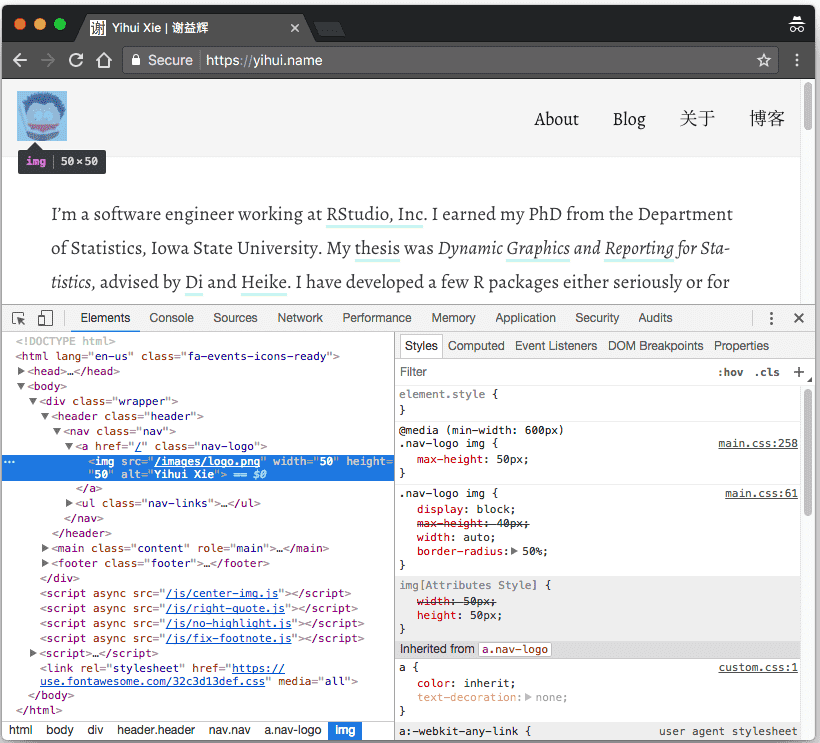
\includegraphics[width=1\linewidth]{images/chrome-devtools} 

}

\caption{Herramientas de desarrollador en Google Chrome.}\label{fig:chrome-devtools}
\end{figure}

Por lo general, también puede abrir las Herramientas de desarrollo
haciendo clic derecho en un elemento determinado en la página web y
seleccionando la opción del menú \texttt{Inspeccionar} (o
\texttt{Inspeccionar\ elemento}). En la figura @ref(fig:
chrome-devtools), hice clic derecho en la imagen de perfil de mi sitio
web \url{https://yihui.name} y lo inspeccioné, y Chrome destacó su
código fuente HTML \texttt{\textless{}img\ src="...".../\textgreater{}}
en el panel izquierdo. También puede ver los estilos CSS asociados con
este elemento \texttt{img} en el panel derecho. Además, puede cambiar
los estilos de forma interactiva si conoce CSS y ver los efectos
(temporales) en tiempo real en la página. Una vez que esté satisfecho
con los nuevos estilos, puede escribir el código CSS en los archivos.

Hay muchas características increíbles de Herramientas de desarrollador,
que las hacen no solo extremadamente útiles para la depuración y la
experimentación, sino también útiles para el aprendizaje del desarrollo
web. Estas herramientas son indispensables para mí cuando desarrollo
algo relacionado con páginas web. Aprendí mucho sobre CSS y JavaScript
jugando con estas herramientas.

\hypertarget{html}{%
\section{HTML}\label{html}}

HTML\index{HTML} significa Hyper Text Markup Language, y es el lenguaje
detrás de la mayoría de las páginas web que usted ve. Puede usar el menú
\texttt{Ver\ -\textgreater{}\ Ver\ fuente} o el menú contextual
\texttt{Ver\ fuente\ de\ página} para ver la fuente HTML completa de una
página web en su navegador. Todos los elementos en una página están
representados por etiquetas HTML. Por ejemplo, la etiqueta
\texttt{\textless{}p\textgreater{}} representa párrafos, y
\texttt{\textless{}img\textgreater{}} representa imágenes.

Lo bueno de HTML es que el lenguaje tiene solo un número limitado de
etiquetas, y el número no es muy grande (especialmente el número de
etiquetas comúnmente utilizadas). Esto significa que hay esperanza de
que pueda dominar este idioma de manera completa y rápida.

La mayoría de las etiquetas HTML aparecen en pares, con una etiqueta de
apertura y una etiqueta de cierre, por ejemplo,
\texttt{\textless{}p\textgreater{}\textless{}/p\textgreater{}}. Usted
escribe el contenido entre las etiquetas de apertura y cierre, por
ejemplo,
\texttt{\textless{}p\textgreater{}Este\ es\ un\ párrafo.\textless{}/\ P\textgreater{}}.
Hay algunas excepciones, como la etiqueta
\texttt{\textless{}img\textgreater{}}, que se puede cerrar con una barra
inclinada \texttt{/} en la etiqueta de apertura, por ejemplo,
\texttt{\textless{}img\ src="foo.png"/\textgreater{}}. Puede especificar
los atributos de un elemento en la etiqueta de apertura usando la
sintaxis \texttt{name=value} (algunos atributos no requieren
\texttt{value}).

Los documentos HTML a menudo tienen la extensión de nombre de archivo
\texttt{.html} (o \texttt{.htm}). A continuación se muestra una
estructura general de un documento HTML:

\begin{Shaded}
\begin{Highlighting}[]
\KeywordTok{<html>}

  \KeywordTok{<head>}
  \KeywordTok{</head>}
  
  \KeywordTok{<body>}
  \KeywordTok{</body>}

\KeywordTok{</html>}
\end{Highlighting}
\end{Shaded}

Básicamente, un documento HTML consta de una sección \texttt{head} y
\texttt{body}. Puede especificar los metadatos e incluir archivos como
archivos CSS en la sección \texttt{head}. Normalmente, la sección
\texttt{head} no está visible en una página web. Es la sección de
`cuerpo' que mantiene el contenido para mostrarse a un lector. A
continuación se muestra un documento de ejemplo un poco más rico:

\begin{Shaded}
\begin{Highlighting}[]
\DataTypeTok{<!DOCTYPE }\NormalTok{html}\DataTypeTok{>}
\KeywordTok{<html>}

  \KeywordTok{<head>}
    \KeywordTok{<meta}\OtherTok{ charset=}\StringTok{"utf-8"} \KeywordTok{/>}
    
    \KeywordTok{<title>}\NormalTok{Your Page Title}\KeywordTok{</title>}
    
    \KeywordTok{<link}\OtherTok{ rel=}\StringTok{"stylesheet"}\OtherTok{ href=}\StringTok{"/css/style.css"} \KeywordTok{/>}
  \KeywordTok{</head>}
  
  \KeywordTok{<body>}
    \KeywordTok{<h1>}\NormalTok{A First-level Heading}\KeywordTok{</h1>}
    
    \KeywordTok{<p>}\NormalTok{A paragraph.}\KeywordTok{</p>}
    
    \KeywordTok{<img}\OtherTok{ src=}\StringTok{"/images/foo.png"}\OtherTok{ alt=}\StringTok{"A nice image"} \KeywordTok{/>}
    
    \KeywordTok{<ul>}
      \KeywordTok{<li>}\NormalTok{An item.}\KeywordTok{</li>}
      \KeywordTok{<li>}\NormalTok{Another item.}\KeywordTok{</li>}
      \KeywordTok{<li>}\NormalTok{Yet another item.}\KeywordTok{</li>}
    \KeywordTok{</ul>}
    
    \KeywordTok{<script}\OtherTok{ src=}\StringTok{"/js/bar.js"}\KeywordTok{></script>}
  \KeywordTok{</body>}

\KeywordTok{</html>}
\end{Highlighting}
\end{Shaded}

En la cabecera, declaramos que la codificación de caracteres de esta
página es UTF-8 a través de una etiqueta
\texttt{\textless{}meta\textgreater{}}, especificamos el título mediante
la etiqueta \texttt{\textless{}title\textgreater{}} e incluimos una hoja
de estilo mediante una etiqueta \texttt{\textless{}link\textgreater{}}.

El cuerpo contiene un encabezado de sección de primer nivel
\texttt{\textless{}h1\textgreater{}},\footnote{Hay seis niveles posibles
  de \texttt{h1}, \texttt{h2}, \ldots{}, a \texttt{h6}.} Un párrafo
\texttt{\textless{}p\textgreater{}}, una imagen
\texttt{\textless{}img\textgreater{}}, una lista desordenada
\texttt{\textless{}ul\textgreater{}} con tres elementos de lista
\texttt{\textless{}li\textgreater{}}, e incluye un archivo JavaScript al
final a través de \texttt{\textless{}script\textgreater{}}.

Hay tutoriales mucho mejores en HTML que esta sección, como los que
ofrecen MDN y w3schools.com, por lo que no vamos a hacer de esta sección
un tutorial completo. En cambio, solo queremos brindar algunos consejos
sobre HTML:

\begin{itemize}
\item
  Puede validar su código HTML a través de este servicio:
  \url{https://validator.w3.org}. Este validador señalará posibles
  problemas de su código HTML. En realidad, también funciona para
  documentos XML y SVG.
\item
  Entre todos los atributos de HTML, las rutas de archivos (el atributo
  \texttt{src} de algunas etiquetas como
  \texttt{\textless{}img\textgreater{}}) y los enlaces (el atributo
  \texttt{href} de la etiqueta \texttt{\textless{}a\textgreater{}})
  pueden ser las más confusas para los principiantes. Las rutas y los
  enlaces pueden ser relativos o absolutos, y pueden venir con o sin el
  protocolo y el dominio. Tiene que entender a qué apunta exactamente un
  enlace o una ruta. Un enlace completo tiene la forma
  \texttt{http://www.example.com/foo/bar.ext}, donde \texttt{http}
  especifica el protocolo (puede tratarse de otros protocolos como
  \texttt{https} o \texttt{ftp}), \texttt{www.example.com} es el
  dominio, y \texttt{foo/bar.ext} es el archivo debajo del directorio
  raíz del sitio web.

  \begin{itemize}
  \item
    Si se refiere a recursos en el mismo sitio web (el mismo protocolo y
    dominio), le recomendamos que omita el protocolo y los nombres de
    dominio, para que los enlaces continúen funcionando incluso si
    cambia el protocolo o dominio. Por ejemplo, un enlace
    \texttt{\textless{}a\ href="/hi/there.html"\textgreater{}} en una
    página \texttt{http://example.com/foo/} hace referencia a
    \texttt{http://example.com/hi/there.html}. No importa si cambia
    \texttt{http} a \texttt{https}, o \texttt{example.com} a
    \texttt{another-domain.com}.
  \item
    Dentro del mismo sitio web, un enlace o ruta puede ser relativa o
    absoluta. El significado de una ruta absoluta no cambia sin importar
    dónde se coloca el archivo HTML actual, pero el significado de una
    ruta relativa depende de la ubicación del archivo HTML actual.
    Supongamos que está viendo la página
    \texttt{example.com/hi/there.html}:
  \item
    Una ruta absoluta \texttt{/foo/bar.ext} siempre significa
    \texttt{example.com/foo/bar.ext}. La barra diagonal significa el
    directorio raíz del sitio web.
  \item
    Una ruta relativa \texttt{../images/foo.png} significa
    \texttt{example.com/images/foo.png} (\texttt{..} significa subir un
    nivel). Sin embargo, si el archivo HTML \texttt{there.html} se mueve
    a \texttt{example.com/hey/again/there.html}, esta ruta en
    \texttt{there.html} se referirá a
    \texttt{example.com/hey/images/foo.png}.
  \item
    Cuando decida si usar rutas relativas o absolutas, aquí está la
    regla general: si no va a mover los recursos referidos o vinculados
    de un subpath a otro (por ejemplo, de \texttt{example.com/foo/} a
    \texttt{example.com/bar/}), pero solo mueve las páginas HTML que
    usan estos recursos, usa rutas absolutas; Si desea cambiar el
    subpaso de la URL de su sitio web, pero las ubicaciones relativas de
    los archivos HTML y los recursos que utilizan no cambian, puede usar
    enlaces relativos (por ejemplo, puede mover todo el sitio web de
    \texttt{example.com/} a \texttt{example.com/foo/}).
  \item
    Si los conceptos anteriores parecen demasiado complicados, una mejor
    manera es pensar detenidamente sobre la estructura de su sitio web y
    evitar mover archivos, o usar reglas de redireccionamientos si son
    compatibles (como los redireccionamientos 301 o 302).
  \item
    Si enlaza a un sitio web o página web diferente, debe incluir el
    dominio en el enlace, pero puede no ser necesario incluir el
    protocolo, por ejemplo, \texttt{//test.example.com/foo.css} es un
    ruta válida. El protocolo real de esta ruta coincide con el
    protocolo de la página actual, por ejemplo, si la página actual es
    \texttt{https://example.com/}, este enlace significa
    \texttt{https://test.example.com/foo.css}. Puede ser beneficioso
    omitir el protocolo porque los recursos HTTP no se pueden incrustar
    en páginas servidas a través de HTTPS (por razones de seguridad),
    por ejemplo, una imagen en \texttt{http://example.com/foo.png} no se
    puede incrustar en una página \texttt{https://example.com/hi.html}
    via
    \texttt{\textless{}img\ src="http://example.com/foo.png"/\textgreater{}},
    pero
    \texttt{\textless{}img\ src="//example.com/foo.png"/\textgreater{}}
    funcionará si se puede acceder a la imagen a través de HTTPS, es
    decir, \texttt{https://example.com/foo.png}. El principal
    inconveniente de no incluir el protocolo es que tales enlaces y
    rutas no funcionan si abre el archivo HTML localmente sin usar un
    servidor web, por ejemplo, solo haga doble clic en el archivo HTML
    en su buscador de archivos y muéstrelo en el navegador.\footnote{Eso
      es porque sin un servidor web, un archivo HTML se ve a través del
      protocolo \texttt{archivo}. Por ejemplo, puede ver una URL del
      formulario \texttt{file://ruta/al/archivo.html} en la barra de
      direcciones de su navegador. La ruta
      \texttt{//example.com/foo.png} se interpretará como
      \texttt{file://example.com/foo.png}, que es poco probable que
      exista como un archivo local en su computadora.}
  \item
    Un error muy común que las personas cometen es poner un enlace sin
    las dobles barras delanteras delante del dominio. Puede pensar que
    \texttt{www.example.com} es un enlace válido. ¡No lo es! Al menos no
    se vincula al sitio web al que desea vincularse. Funciona cuando lo
    escribe en la barra de direcciones de su navegador porque su
    navegador normalmente lo autocompletará en
    \texttt{http://www.example.com}. Sin embargo, si escribe un enlace
    \texttt{\textless{}a\ href="www.example.com"\textgreater{}Vea\ este\ enlace\textless{}/a\textgreater{}},
    tendrá problemas. El navegador interpretará esto como un enlace
    relativo, y es relativo a la URL de la página web actual, por
    ejemplo, si actualmente está viendo \texttt{http://yihui.name/cn/},
    el enlace \texttt{www.example.com} en realidad significa
    \texttt{http://yihui.name/cn/www.example.com}! Ahora debería conocer
    el texto de Markdown \texttt{{[}Link{]}(www.example.com)} suele ser
    un error, a menos que realmente quiera vincular un subdirectorio de
    la página actual o un archivo con literalmente el nombre
    \texttt{www.example.com}.
  \end{itemize}
\end{itemize}

\hypertarget{css}{%
\section{CSS}\label{css}}

El lenguaje Cascading Stylesheets \index{CSS} (CSS) se utiliza para
describir el aspecto y el formato de los documentos escritos en HTML.
CSS es responsable del estilo visual de su sitio. CSS es muy divertido
de jugar, pero también puede robar tu tiempo fácilmente.

En el marco de Hugo
(\url{https://gohugo.io/tutorials/creating-a-new-theme/}), CSS es uno de
los principales archivos ``sin contenido'' que da forma a la apariencia
de su sitio (los otros son imágenes, JavaScript y plantillas Hugo). ¿Qué
significa el
\href{https://en.wikipedia.org/wiki/Look_and_feel}{``aspecto y tacto''}
de un sitio? ``Buscar'' generalmente se refiere a componentes de estilo
estático que incluyen, entre otros,

\begin{itemize}
\tightlist
\item
  paltetas de color,
\item
  imágenes,
\item
  diseños/márgenes, y
\item
  fuentes.
\end{itemize}

mientras que ``sentir'' se relaciona con componentes dinámicos con los
que el usuario interactúa como

\begin{itemize}
\tightlist
\item
  menús desplegables,
\item
  botones, y
\item
  formas.
\end{itemize}

Hay 3 formas de definir estilos. El primero está en línea con HTML. Por
ejemplo, este código

\begin{Shaded}
\begin{Highlighting}[]
\KeywordTok{<p>}\NormalTok{Marco! }\KeywordTok{<em>}\NormalTok{Polo!}\KeywordTok{</em></p>} 
\end{Highlighting}
\end{Shaded}

produciría texto que se parece a esto: Marco! \emph{Polo!}

Sin embargo, este método generalmente no es preferido para
\href{https://stackoverflow.com/q/12013532/559676}{razones numerosas.}

Una segunda forma es definir internamente el CSS colocando una sección
de estilo en su HTML:

\begin{Shaded}
\begin{Highlighting}[]
\KeywordTok{<html>}
\KeywordTok{<style>} 
\PreprocessorTok{#favorite}\NormalTok{ \{}
    \KeywordTok{font-style}\NormalTok{: }\DecValTok{italic}\NormalTok{;}
\NormalTok{\}}
\KeywordTok{</style>}
\KeywordTok{<ul}\OtherTok{ id=}\StringTok{"tea-list"}\KeywordTok{>}
  \KeywordTok{<li>}\NormalTok{Earl Grey}\KeywordTok{</li>}
  \KeywordTok{<li>}\NormalTok{Darjeeling}\KeywordTok{</li>}
  \KeywordTok{<li>}\NormalTok{Oolong}\KeywordTok{</li>}
  \KeywordTok{<li>}\NormalTok{Chamomile}\KeywordTok{</li>}
  \KeywordTok{<li}\OtherTok{ id=}\StringTok{"favorite"}\KeywordTok{>}\NormalTok{Chai}\KeywordTok{</li>}
\KeywordTok{</ul>}
\KeywordTok{</html>}
\end{Highlighting}
\end{Shaded}

En este ejemplo, solo el último té enumerado, \emph{Chai}, está en
cursiva.

El tercer método es el más popular porque es más flexible y el menos
repetitivo. En este método, usted define el CSS en un archivo externo
que luego se referencia como un enlace en su HTML:

\begin{Shaded}
\begin{Highlighting}[]
\KeywordTok{<html>}
    \KeywordTok{<link}\OtherTok{ rel=}\StringTok{"stylesheet"}\OtherTok{ href=}\StringTok{"/css/style.css"} \KeywordTok{/>}
\KeywordTok{</html>}
\end{Highlighting}
\end{Shaded}

Lo que va dentro del documento CSS vinculado es esencialmente una lista
de reglas (la misma lista podría aparecer internamente entre las
etiquetas de estilo, si está utilizando el segundo método). Cada regla
debe incluir un selector o un grupo de selectores, y un bloque de
declaraciones dentro de llaves que contenga uno o más pares
\texttt{property:\ value;}. Aquí está la
\href{https://developer.mozilla.org/en-US/docs/Web/CSS/Reference}{estructura
general para una regla}:

\begin{Shaded}
\begin{Highlighting}[]
\CommentTok{/* CSS pseudo-code */}
\NormalTok{selectorlist \{}
\NormalTok{    property: value;}
    \CommentTok{/* more property: value; pairs*/}
\NormalTok{\}}
\end{Highlighting}
\end{Shaded}

Los
\href{https://developer.mozilla.org/en-US/docs/Web/CSS/Reference\#Selectors}{selectores}
pueden basarse en tipos o atributos de elementos HTML, como \texttt{id}
o \texttt{class} (y combinaciones de estos atributos):

\begin{Shaded}
\begin{Highlighting}[]
\CommentTok{/* by element type */}
\NormalTok{li \{ }
    \KeywordTok{color}\NormalTok{: }\DecValTok{yellow}\NormalTok{; }\CommentTok{/* all <li> elements are yellow */}
\NormalTok{\}}

\CommentTok{/* by ID with the # symbol */}
\PreprocessorTok{#my-id}\NormalTok{ \{ }
    \KeywordTok{color}\NormalTok{: }\DecValTok{yellow}\NormalTok{; }\CommentTok{/* elements with id = "my-id" are yellow */}
\NormalTok{\}}

\CommentTok{/* by class with the . symbol */}
\FunctionTok{.my-class}\NormalTok{ \{ }
    \KeywordTok{color}\NormalTok{: }\DecValTok{yellow}\NormalTok{; }\CommentTok{/* elements with class = "my-class" are yellow  */}
\NormalTok{\}}
\end{Highlighting}
\end{Shaded}

Debido a que cada elemento HTML puede coincidir con varios selectores
diferentes, el estándar CSS determina qué conjunto de reglas tiene
prioridad para cualquier elemento dado y qué propiedades heredar. Aquí
es donde el algoritmo de cascada entra en juego. Por ejemplo, tome una
lista desordenada simple:

\begin{Shaded}
\begin{Highlighting}[]
\KeywordTok{<ul}\OtherTok{ id=}\StringTok{"tea-list"}\KeywordTok{>}
  \KeywordTok{<li>}\NormalTok{Earl Grey}\KeywordTok{</li>}
  \KeywordTok{<li>}\NormalTok{Darjeeling}\KeywordTok{</li>}
  \KeywordTok{<li>}\NormalTok{Oolong}\KeywordTok{</li>}
  \KeywordTok{<li>}\NormalTok{Chamomile}\KeywordTok{</li>}
  \KeywordTok{<li>}\NormalTok{Chai}\KeywordTok{</li>}
\KeywordTok{</ul>}
\end{Highlighting}
\end{Shaded}

Ahora, digamos que queremos resaltar nuestros tés favoritos nuevamente,
así que usaremos un atributo de clase.

\begin{Shaded}
\begin{Highlighting}[]
\KeywordTok{<ul}\OtherTok{ id=}\StringTok{"tea-list"}\KeywordTok{>}
  \KeywordTok{<li>}\NormalTok{Earl Grey}\KeywordTok{</li>}
  \KeywordTok{<li}\OtherTok{ class=}\StringTok{"favorite"}\KeywordTok{>}\NormalTok{Darjeeling}\KeywordTok{</li>}
  \KeywordTok{<li>}\NormalTok{Oolong}\KeywordTok{</li>}
  \KeywordTok{<li>}\NormalTok{Chamomile}\KeywordTok{</li>}
  \KeywordTok{<li}\OtherTok{ class=}\StringTok{"favorite"}\KeywordTok{>}\NormalTok{Chai}\KeywordTok{</li>}
\KeywordTok{</ul>}
\end{Highlighting}
\end{Shaded}

Podemos usar este atributo de clase como un selector en nuestro CSS.
Digamos que queremos que nuestros tés favoritos estén en negrita y
tengan un color de fondo amarillo, por lo que nuestro CSS se vería así:

\begin{Shaded}
\begin{Highlighting}[]
\FunctionTok{.favorite}\NormalTok{ \{}
  \KeywordTok{font-weight}\NormalTok{: }\DecValTok{bold}\NormalTok{;}
  \KeywordTok{background-color}\NormalTok{: }\DecValTok{yellow}\NormalTok{;}
\NormalTok{\}}
\end{Highlighting}
\end{Shaded}

Ahora, si desea que cada elemento de la lista se ponga en cursiva con un
fondo blanco, puede configurar otra regla:

\begin{Shaded}
\begin{Highlighting}[]
\NormalTok{li \{ }
  \KeywordTok{font-style}\NormalTok{: }\DecValTok{italic}\NormalTok{;}
  \KeywordTok{background-color}\NormalTok{: }\DecValTok{white}\NormalTok{;}
\NormalTok{\}}
\end{Highlighting}
\end{Shaded}

Si juega con este código (que puede usar fácilmente usando sitios como
\url{http://jsbin.com}, \url{https://jsfiddle.net} o
\url{https://codepen.io/pen/}), verá que el segundo té favorito sigue
resaltado en amarillo. Esto se debe a que la regla de CSS sobre
\texttt{.favorite} como clase es más específica que la regla sobre
elementos de tipo \texttt{li}. Para anular la regla \texttt{.favorite},
debe ser tan específico como sea posible al elegir su grupo de
selectores:

\begin{Shaded}
\begin{Highlighting}[]
\NormalTok{ul}\PreprocessorTok{#tea-list}\NormalTok{ li}\FunctionTok{.favorite}\NormalTok{ \{}
  \KeywordTok{background-color}\NormalTok{: }\DecValTok{white}\NormalTok{;}
\NormalTok{\}}
\end{Highlighting}
\end{Shaded}

Este ejemplo solo araña la superficie de
\href{https://developer.mozilla.org/en-US/docs/Learn/CSS/Introduction_to_CSS/Cascade_and_inheritance}{cascada
y herencia.}

Para cualquier tema de Hugo que instale, puede encontrar el archivo CSS
en la carpeta \texttt{themes/}. Por ejemplo, el tema predeterminado de
litio se encuentra en:
\texttt{themes/hugo-lithium-theme/static/css/main.css}. Una vez que esté
familiarizado con CSS, puede comprender cómo funciona cada conjunto de
reglas para dar forma al estilo visual de su sitio web, y cómo modificar
las reglas. Para algunos temas (es decir, el
\href{https://github.com/gcushen/hugo-academic}{tema académico}), tiene
la opción de vincular a un
\href{https://gist.github.com/gcushen/d5525a4506b9ccf83f2bce592a895495}{CSS
personalizado} que puede utilizar para personalizar aún más el estilo
visual de su sitio.

Algunos ejemplos de una línea ilustran cómo las simples reglas de CSS se
pueden usar para hacer cambios dramáticos:

\begin{itemize}
\item
  Para hacer imágenes circulares o redondeadas, puede asignar una clase
  \texttt{img-circle} a imágenes (e.g.,
  \texttt{\textless{}img\ class="img-circle"\ src="foo.png"\ /\textgreater{}})
  y definir el CSS:

\begin{Shaded}
\begin{Highlighting}[]
\FunctionTok{.img-circle}\NormalTok{ \{}
  \KeywordTok{border-radius}\NormalTok{: }\DecValTok{50%}\NormalTok{;}
\NormalTok{\}}
\end{Highlighting}
\end{Shaded}
\item
  Para hacer tablas de rayas, puede agregar colores de fondo a las filas
  impares o pares de la tabla, e.g.,

\begin{Shaded}
\begin{Highlighting}[]
\NormalTok{tr}\InformationTok{:nth-child}\NormalTok{(even) \{}
  \KeywordTok{background}\NormalTok{: }\DecValTok{#eee}\NormalTok{;}
\NormalTok{\}}
\end{Highlighting}
\end{Shaded}
\item
  Puede agregar o anteponer contenido a elementos a través de
  pseudo-elementos \texttt{::after} y \texttt{::before}. Aquí hay un
  ejemplo de cómo agregar un período después de los números de sección:
  \url{https://github.com/rstudio/blogdown/issues/80}.
\end{itemize}

\hypertarget{javascript}{%
\section{JavaScript}\label{javascript}}

Es mucho más difícil introducir JavaScript \index{JavaScript} que HTML y
CSS, ya que es un lenguaje de programación. Hay muchos libros y
tutoriales sobre este idioma. De todos modos, intentaremos arañar la
superficie para los usuarios R en esta sección.

En pocas palabras, JavaScript es un lenguaje que generalmente se utiliza
para manipular elementos en una página web. Una forma efectiva de
aprender es a través de la consola de JavaScript en las Herramientas de
Desarrollador de su navegador web (vea la Figura @ref(fig:
chrome-devtools)), porque puede escribir código de manera interactiva en
la consola y ejecutarlo, lo cual se siente similar para ejecutar el
código en R en la consola de R (por ejemplo, en RStudio). Puede abrir
cualquier página web en su navegador web (por ejemplo,
\url{https://yihui.name}), luego abrir la consola de JavaScript y probar
el siguiente código en cualquier página web:

\begin{Shaded}
\begin{Highlighting}[]
\VariableTok{document}\NormalTok{.}\VariableTok{body}\NormalTok{.}\VariableTok{style}\NormalTok{.}\AttributeTok{background} \OperatorTok{=} \StringTok{'orange'}\OperatorTok{;}
\end{Highlighting}
\end{Shaded}

Debería cambiar el color de fondo de la página a naranja, a menos que la
página ya haya definido los colores de fondo para ciertos elementos.

Para usar JavaScript de manera efectiva, debe aprender tanto la sintaxis
básica de JavaScript como la forma de seleccionar elementos en una
página antes de poder manipularlos. Puede aprender parcialmente lo
primero a partir del fragmento corto de JavaScript a continuación:

\begin{Shaded}
\begin{Highlighting}[]
\KeywordTok{var}\NormalTok{ x }\OperatorTok{=} \DecValTok{1}\OperatorTok{;}  \CommentTok{// assignments}
\DecValTok{1} \OperatorTok{+} \DecValTok{2} \OperatorTok{-} \DecValTok{3} \OperatorTok{*} \DecValTok{4}\NormalTok{ / }\DecValTok{5}\OperatorTok{;}  \CommentTok{// arithmetic}

\ControlFlowTok{if}\NormalTok{ (x }\OperatorTok{<} \DecValTok{2}\NormalTok{) }\VariableTok{console}\NormalTok{.}\AttributeTok{log}\NormalTok{(x)}\OperatorTok{;}  \CommentTok{// "print" x}

\KeywordTok{var}\NormalTok{ y }\OperatorTok{=}\NormalTok{ [}\DecValTok{9}\OperatorTok{,} \DecValTok{1}\OperatorTok{,} \DecValTok{0}\OperatorTok{,} \DecValTok{2}\OperatorTok{,} \DecValTok{1}\OperatorTok{,} \DecValTok{4}\NormalTok{]}\OperatorTok{;}  \CommentTok{// array}

\CommentTok{// function}
\KeywordTok{var}\NormalTok{ sum }\OperatorTok{=} \KeywordTok{function}\NormalTok{(x) }\OperatorTok{\{}
  \KeywordTok{var}\NormalTok{ s }\OperatorTok{=} \DecValTok{0}\OperatorTok{;}
  \CommentTok{// a naive way to compute the sum}
  \ControlFlowTok{for}\NormalTok{ (}\KeywordTok{var}\NormalTok{ i}\OperatorTok{=}\DecValTok{0}\OperatorTok{;}\NormalTok{ i }\OperatorTok{<} \VariableTok{x}\NormalTok{.}\AttributeTok{length}\OperatorTok{;}\NormalTok{ i}\OperatorTok{++}\NormalTok{) }\OperatorTok{\{}
\NormalTok{    s }\OperatorTok{+=}\NormalTok{ x[i]}\OperatorTok{;}
  \OperatorTok{\}}
  \ControlFlowTok{return}\NormalTok{ s}\OperatorTok{;}
\OperatorTok{\};}

\AttributeTok{sum}\NormalTok{(y)}\OperatorTok{;}

\KeywordTok{var}\NormalTok{ y }\OperatorTok{=} \StringTok{"Hello World"}\OperatorTok{;}
\NormalTok{y }\OperatorTok{=} \VariableTok{y}\NormalTok{.}\AttributeTok{replace}\NormalTok{(}\StringTok{" "}\OperatorTok{,} \StringTok{", "}\NormalTok{)}\OperatorTok{;}  \CommentTok{// string manipulation}
\end{Highlighting}
\end{Shaded}

Puede sentir que la sintaxis es similar a R hasta cierto punto.
JavaScript es un lenguaje orientado a objetos, y generalmente hay varios
métodos que puede aplicar a un objeto. La manipulación de cadena
anterior es un ejemplo típico de la sintaxis \texttt{Object.method()}.
Para conocer los métodos posibles en un objeto, puede escribir el nombre
del objeto en su consola JavaScript seguido de un punto, y debería ver
todos los candidatos.

Los usuarios de R deben ser extremadamente cautelosos porque los objetos
JavaScript a menudo son mutables, lo que significa que un objeto puede
ser modificado en cualquier lugar. A continuación, hay un ejemplo
rápido:

\begin{Shaded}
\begin{Highlighting}[]
\KeywordTok{var}\NormalTok{ x }\OperatorTok{=} \OperatorTok{\{}\StringTok{"a"}\OperatorTok{:} \DecValTok{1}\OperatorTok{,} \StringTok{"b"}\OperatorTok{:} \DecValTok{2}\OperatorTok{\};}  \CommentTok{// como una lista en R}
\KeywordTok{var}\NormalTok{ f }\OperatorTok{=} \KeywordTok{function}\NormalTok{(z) }\OperatorTok{\{}
  \VariableTok{z}\NormalTok{.}\AttributeTok{a} \OperatorTok{=} \DecValTok{100}\OperatorTok{;}
\OperatorTok{\};}
\AttributeTok{f}\NormalTok{(x)}\OperatorTok{;}
\NormalTok{x}\OperatorTok{;}  \CommentTok{// modificado! x.a es 100 ahora}
\end{Highlighting}
\end{Shaded}

Hay muchas librerías maduras de JavaScript que pueden ayudarlo a
seleccionar y manipular elementos en una página, y la más popular puede
ser\index{jQuery} \href{https://jquery.com}{jQuery.} Sin embargo, debe
saber que a veces probablemente puede hacerlo lo suficientemente bien
sin estas librerías de terceros. Hay algunos métodos básicos para
seleccionar elementos, como \texttt{document.getElementById()} y
\texttt{document.getElementsByClassName()}. Por ejemplo, puede
seleccionar todos los párrafos usando
\texttt{document.querySelectorAll(\textquotesingle{}p\textquotesingle{})}.

A continuación mostramos una aplicación ligeramente avanzada, en la que
verá funciones anónimas, selección de elementos por nombres de etiquetas
HTML, expresiones regulares y manipulación de elementos HTML.

En la sección \ref{how-to}, mencionamos cómo habilitar
MathJax\index{MathJax} en un sitio web de Hugo. La parte fácil es
incluir el script \texttt{MathJax.js} a través de una etiqueta
\texttt{\textless{}script\textgreater{}}, y hay dos partes difíciles:

\begin{enumerate}
\def\labelenumi{\arabic{enumi}.}
\item
  Cómo proteger el contenido matemático del motor de reducción
  (Blackfriday), por ejemplo, necesitamos asegurarnos de que los
  subrayados en las expresiones matemáticas no se interpreten como
  \texttt{\textless{}em\textgreater{}\textless{}/em\textgreater{}}. Este
  problema solo existe en las publicaciones simples de Markdown, y se ha
  mencionado en la sección \ref{formato-de-salida} sin explicar la
  solución.
\item
  Por defecto, MathJax no reconoce un par de signos de pesos como la
  sintaxis de las expresiones matemáticas en línea, pero la mayoría de
  los usuarios se sienten más cómodos con la sintaxis \texttt{\$x\$} que
  con \texttt{\textbackslash{}(x\textbackslash{})}.
\end{enumerate}

La solución más fácil para el primer problema puede ser la adición de
retrocesos alrededor de las expresiones matemáticas, por ejemplo,
\texttt{\textasciigrave{}\$x\_i\$\textasciigrave{}}, pero la
consecuencia es que la expresión matemática se representará en
\texttt{\textless{}code\textgreater{}\textless{}/code\textgreater{}}, y
MathJax ignora las etiquetas \texttt{\textless{}code\textgreater{}}
cuando busca expresiones matemáticas en la página. Podemos obligar a
MathJax a buscar expresiones matemáticas en
\texttt{\textless{}code\textgreater{}}, pero esto seguirá siendo
problemático. Por ejemplo, alguien puede querer mostrar el código en
línea R \texttt{\textasciigrave{}list\$x\$y\textasciigrave{}}, y
\texttt{\$x\$} puede reconocerse como una expresión matemática. MathJax
ignora \texttt{\textless{}code\textgreater{}} por buenas razones.
Incluso si no tiene esas expresiones en
\texttt{\textless{}code\textgreater{}}, puede tener algunos estilos CSS
especiales adjuntos a \texttt{\textless{}code\textgreater{}}, y estos
estilos se aplicarán a sus expresiones matemáticas, que pueden ser no
deseadas (por ejemplo, una luz fondo gris).

Para resolver estos problemas, proporcioné una solución en el código
JavaScript en \url{https://yihui.name/js/math-code.js}:

\begin{Shaded}
\begin{Highlighting}[]
\NormalTok{(}\KeywordTok{function}\NormalTok{() }\OperatorTok{\{}
  \KeywordTok{var}\NormalTok{ i}\OperatorTok{,}\NormalTok{ text}\OperatorTok{,}\NormalTok{ code}\OperatorTok{,}\NormalTok{ codes }\OperatorTok{=} \VariableTok{document}\NormalTok{.}\AttributeTok{getElementsByTagName}\NormalTok{(}\StringTok{'code'}\NormalTok{)}\OperatorTok{;}
  \ControlFlowTok{for}\NormalTok{ (i }\OperatorTok{=} \DecValTok{0}\OperatorTok{;}\NormalTok{ i }\OperatorTok{<} \VariableTok{codes}\NormalTok{.}\AttributeTok{length}\OperatorTok{;}\NormalTok{) }\OperatorTok{\{}
\NormalTok{    code }\OperatorTok{=}\NormalTok{ codes[i]}\OperatorTok{;}
    \ControlFlowTok{if}\NormalTok{ (}\VariableTok{code}\NormalTok{.}\VariableTok{parentNode}\NormalTok{.}\AttributeTok{tagName} \OperatorTok{!==} \StringTok{'PRE'} \OperatorTok{&&}
        \VariableTok{code}\NormalTok{.}\AttributeTok{childElementCount} \OperatorTok{===} \DecValTok{0}\NormalTok{) }\OperatorTok{\{}
\NormalTok{      text }\OperatorTok{=} \VariableTok{code}\NormalTok{.}\AttributeTok{textContent}\OperatorTok{;}
      \ControlFlowTok{if}\NormalTok{ (}\SpecialStringTok{/}\SpecialCharTok{^\textbackslash{}$[^$]}\SpecialStringTok{/}\NormalTok{.}\AttributeTok{test}\NormalTok{(text) }\OperatorTok{&&} \SpecialStringTok{/}\SpecialCharTok{[^$]\textbackslash{}$$}\SpecialStringTok{/}\NormalTok{.}\AttributeTok{test}\NormalTok{(text)) }\OperatorTok{\{}
\NormalTok{        text }\OperatorTok{=} \VariableTok{text}\NormalTok{.}\AttributeTok{replace}\NormalTok{(}\SpecialStringTok{/}\SpecialCharTok{^\textbackslash{}$}\SpecialStringTok{/}\OperatorTok{,} \StringTok{'}\SpecialCharTok{\textbackslash{}\textbackslash{}}\StringTok{('}\NormalTok{).}\AttributeTok{replace}\NormalTok{(}\SpecialStringTok{/}\SpecialCharTok{\textbackslash{}$$}\SpecialStringTok{/}\OperatorTok{,} \StringTok{'}\SpecialCharTok{\textbackslash{}\textbackslash{}}\StringTok{)'}\NormalTok{)}\OperatorTok{;}
        \VariableTok{code}\NormalTok{.}\AttributeTok{textContent} \OperatorTok{=}\NormalTok{ text}\OperatorTok{;}
      \OperatorTok{\}}
      \ControlFlowTok{if}\NormalTok{ (}\SpecialStringTok{/}\SpecialCharTok{^\textbackslash{}\textbackslash{}\textbackslash{}((}\SpecialStringTok{.}\SpecialCharTok{|\textbackslash{}s)+\textbackslash{}\textbackslash{}\textbackslash{})$}\SpecialStringTok{/}\NormalTok{.}\AttributeTok{test}\NormalTok{(text) }\OperatorTok{||}
          \SpecialStringTok{/}\SpecialCharTok{^\textbackslash{}\textbackslash{}\textbackslash{}[(}\SpecialStringTok{.}\SpecialCharTok{|\textbackslash{}s)+\textbackslash{}\textbackslash{}\textbackslash{}]$}\SpecialStringTok{/}\NormalTok{.}\AttributeTok{test}\NormalTok{(text) }\OperatorTok{||}
          \SpecialStringTok{/}\SpecialCharTok{^\textbackslash{}$(}\SpecialStringTok{.}\SpecialCharTok{|\textbackslash{}s)+\textbackslash{}$$}\SpecialStringTok{/}\NormalTok{.}\AttributeTok{test}\NormalTok{(text) }\OperatorTok{||}
          \SpecialStringTok{/}\SpecialCharTok{^\textbackslash{}\textbackslash{}}\SpecialStringTok{begin}\SpecialCharTok{\textbackslash{}\{([^\}]+)\textbackslash{}\}(}\SpecialStringTok{.}\SpecialCharTok{|\textbackslash{}s)+\textbackslash{}\textbackslash{}}\SpecialStringTok{end}\SpecialCharTok{\textbackslash{}\{[^\}]+\textbackslash{}\}$}\SpecialStringTok{/}\NormalTok{.}\AttributeTok{test}\NormalTok{(text)) }\OperatorTok{\{}
        \VariableTok{code}\NormalTok{.}\AttributeTok{outerHTML} \OperatorTok{=} \VariableTok{code}\NormalTok{.}\AttributeTok{innerHTML}\OperatorTok{;}  \CommentTok{// remove <code></code>}
        \ControlFlowTok{continue}\OperatorTok{;}
      \OperatorTok{\}}
    \OperatorTok{\}}
\NormalTok{    i}\OperatorTok{++;}
  \OperatorTok{\}}
\OperatorTok{\}}\NormalTok{)()}\OperatorTok{;}
\end{Highlighting}
\end{Shaded}

No es una solución perfecta, pero debería ser muy raro que tenga
problemas. Esta solución identifica posibles expresiones matemáticas en
\texttt{\textless{}code\textgreater{}}, y elimina la etiqueta
\texttt{\textless{}code\textgreater{}}, por ejemplo, reemplaza
\texttt{\textless{}code\textgreater{}\$x\$\textless{}/code\textgreater{}}
con \texttt{\textbackslash{}(x\textbackslash{})}. Después de que se
ejecuta este script, cargamos el script MathJax. De esta forma, no
necesitamos obligar a MathJax a buscar expresiones matemáticas en las
etiquetas \texttt{\textless{}code\textgreater{}}, y sus expresiones
matemáticas no heredarán ningún estilo de
\texttt{\textless{}code\textgreater{}}. El código de JavaScript anterior
no es demasiado largo y debe ser autoexplicativo. La parte más difícil
es \texttt{i++}. Dejaré que los lectores descubran por qué el bucle
\texttt{for} no es la forma
habitual\texttt{for(i\ =\ 0;\ i\ \textless{}codes.length;\ i\ ++)}. Me
tomó unos minutos darme cuenta de mi error cuando escribí el ciclo en la
forma habitual.

\hypertarget{recursos-utiles}{%
\section{Recursos útiles}\label{recursos-utiles}}

\hypertarget{organizacion-de-archivos}{%
\subsection{Organización de archivos}\label{organizacion-de-archivos}}

Aunque los sitios web estáticos de \index{Optimización} son rápidos en
general, ciertamente puede optimizarlos aún más. Puede buscar
``minificador de CSS y JavaScript'', y estas herramientas pueden
comprimir sus archivos CSS y JavaScript, de modo que puedan cargarse más
rápido. Como hay muchas herramientas, no las recomendaré aquí.

También puede optimizar imágenes en su sitio web. Frecuentemente uso una
herramienta de línea de comandos llamada
\href{http://optipng.sourceforge.net}{\texttt{optipng}} para optimizar
las imágenes PNG. Es un optimizador sin pérdida, lo que significa que
reduce el tamaño del archivo de una imagen PNG sin pérdida de calidad.
Desde mi experiencia, funciona muy bien en imágenes PNG generadas a
partir de R, y puede reducir el tamaño del archivo en al menos un 30\%
(a veces incluso más del 50\%). Personalmente también uso herramientas
en línea como \url{http://optimizilla.com} para optimizar imágenes PNG y
JPEG. Para imágenes GIF, a menudo uso \url{https://ezgif.com/optimize}
para reducir el tamaño de los archivos si son demasiado grandes.

Tenga en cuenta que Netlify ha proporcionado las funciones de
optimización en el servidor de forma gratuita en este momento, por lo
que es posible que desee habilitarlos allí en lugar de hacer todo el
trabajo por su cuenta.

\hypertarget{ayudando-a-las-personas-a-encontrar-su-sitio}{%
\subsection{Ayudando a las personas a encontrar su
sitio}\label{ayudando-a-las-personas-a-encontrar-su-sitio}}

Una vez que su sitio esté en funcionamiento, es probable que desee que
las personas lo encuentren. SEO --- Search Engine Optimization --- es el
arte de hacer que un sitio web sea fácil de entender para los motores de
búsqueda como Google. Y, con suerte, si el motor de búsqueda sabe de lo
que está escribiendo, presentará enlaces a su sitio con altos resultados
cuando alguien busque los temas que cubre.

Se han escrito libros completos sobre SEO, sin mencionar las muchas
empresas que se dedican a ofrecer asesoramiento técnico y estratégico
(pagado) para ayudar a que los sitios estén en la cima de los rankings
de los motores de búsqueda. Si está interesado en obtener más
información, un buen lugar para comenzar es la Guía de inicio de la
optimización del motor de búsqueda de Google
(\url{http://bit.ly/google-seo-starter}). A continuación hay algunos
puntos clave:

\begin{enumerate}
\def\labelenumi{\arabic{enumi}.}
\item
  El título que seleccione para cada página y publicación es una señal
  muy importante para Google y otros motores de búsqueda que les dicen
  de qué se trata esa página.
\item
  Las etiquetas de descripción también son fundamentales para explicar
  de qué se trata una página. En documentos HTML,
  \href{https://www.w3schools.com/tags/tag_meta.asp}{etiquetas de
  descripción} son una forma de proporcionar metadatos sobre la página.
  Con \textbf{blogdown}, la descripción puede terminar como texto debajo
  del título de la página en un resultado de motor de búsqueda. Si el
  YAML de su página no incluye una descripción, puede agregar uno como
  \texttt{description:"Una\ breve\ descripción\ de\ esta\ página."}; la
  fuente HTML de la página renderizada tendría una etiqueta
  \texttt{\textless{}meta\textgreater{}} en
  \texttt{\textless{}head\textgreater{}} como
  \texttt{\textless{}meta\ name="description"\ content="\ Una\ breve\ descripción\ de\ esta\ página."\textgreater{}}.
  No todos los temas admiten agregar la descripción a su página HTML
  (¡aunque deberían!)
\item
  La estructura de URL también es importante. Desea que el slug de su
  publicación tenga palabras clave informativas, lo que le da otra señal
  de lo que trata la página. ¿Tiene una publicación con cosas
  interesantes que hacer en San Francisco?
  \texttt{san-francisco-events-calendar} podría ser un mejor slug que
  \texttt{my-guide-to-fun-things-to-do}.
\end{enumerate}

\hypertarget{nombre-de-dominio}{%
\chapter{Nombre de dominio}\label{nombre-de-dominio}}

Si bien puede usar los nombres de subdominio gratuitos
\index{Nombre de dominio} como los provistos por GitHub o Netlify, puede
ser una mejor idea tener un nombre de dominio propio. El costo de un
dominio principal es mínimo (por lo general, el costo anual es de
alrededor de US\$ 10), y usted ingresará a un mundo mucho más rico
después de comprar un nombre de dominio. Por ejemplo, puede colocar su
dominio en cualquier servidor web, puede crear tantos nombres de
subdominios como desee e incluso puede configurar sus propias cuentas de
correo electrónico usando el dominio o los subdominios. En este
apéndice, explicaremos algunos conceptos básicos de nombres de dominio y
mencionaremos algunos servicios (gratuitos) para ayudarlo a configurar
su nombre de dominio.

Antes de sumergirnos en los detalles, queremos delinear la gran imagen
de cómo funciona una URL en su navegador web. Supongamos que escribió o
hizo clic en un enlace \texttt{http://www.example.com/foo/index.html} en
su navegador web. ¿Qué sucede tras bambalinas antes de ver la página web
real?

Primero, el nombre de dominio debe ser resuelto a través de los
servidores de nombres asociados con él. Un servidor de nombres conoce
los registros DNS (Sistema de nombres de dominio) de un dominio. Por lo
general, buscará los ``registros A'' para señalar el dominio a la
dirección IP de un servidor web. Existen muchos otros tipos de registros
DNS, y los explicaremos más adelante. Una vez que se llega al servidor
web, el servidor buscará el archivo \texttt{foo/index.html} debajo de un
directorio asociado con el nombre de dominio, y devolverá su contenido
en la respuesta. Eso es básicamente cómo puedes ver una página web.

\hypertarget{registro}{%
\section{Registro}\label{registro}}

Puede comprar un nombre de dominio de muchos registradores de nombres de
dominio. Para permanecer neutral, no vamos a hacer recomendaciones aquí.
Puede usar su buscador para buscar un registrador por su cuenta, o
pedirle recomendaciones a sus amigos. Sin embargo, nos gustaría
recordarle algunas cosas a las que debe prestar atención cuando busque
un registrador de nombres de dominio:

\begin{itemize}
\item
  Debería tener la libertad de transferir su dominio del registrador
  actual a otros registradores, es decir, no deberían bloquearlo en su
  sistema. Para transferir un nombre de dominio, se le debe dar un
  código conocido como ``Código de transferencia de autenticación'' o
  ``Código de autenticación'' o ``Clave de transferencia'' o algo por el
  estilo.
\item
  Debería poder personalizar los servidores de nombres (consulte la
  sección \ref{nombres-de-servidores}) de su dominio. De forma
  predeterminada, cada registrador le asignará sus propios nombres de
  servidores, y estos nombres de servidores generalmente funcionan muy
  bien. Sin embargo, hay algunos nombres de servidores especiales que
  proporcionan servicios más que solo registros DNS, y puede que esté
  interesado en usarlos.
\item
  Otras personas pueden buscar libremente su información personal, como
  su correo electrónico o dirección postal, después de registrar un
  dominio y enviar esta información al registrador. Esto se denomina
  ``WHOIS Lookup''. Es posible que desee proteger su privacidad, pero su
  registrador puede requerir un pago adicional.
\end{itemize}

\hypertarget{nombres-de-servidores}{%
\section{Nombres de servidores}\label{nombres-de-servidores}}

La razón principal por la que necesitamos nombres de servidores
\index{Nombres de servidores} es que queremos usar dominios en lugar de
direcciones IP, aunque un dominio no es estrictamente necesario para que
pueda acceder a un sitio web. Puede usar la dirección IP si tiene su
propio servidor con una IP pública, pero hay muchos problemas con este
enfoque. Por ejemplo, las direcciones IP son limitadas (en particular,
la IPv4), no son fáciles de memorizar y solo puede alojar un sitio web
por dirección IP (sin utilizar otros puertos).

Un nombre de servidor de nombres es un motor que dirige los registros
DNS de su dominio. El registro DNS más común es el registro A, que
asigna un dominio a una dirección IP, de modo que el servidor de
alojamiento se puede encontrar a través de su dirección IP cuando se
accede a un sitio web a través de un dominio. Presentaremos dos tipos
más de registros DNS en la sección \ref{registros-dns}: registros CNAME
y MX.

En la mayoría de los casos, los nombres de servidores predeterminados
provistos por el registrador de su dominio deberían ser suficientes,
pero falta una tecnología especial en la mayoría de nombres de
servidores: aplanamiento CNAME. Solo necesita esta tecnología si desea
establecer un registro CNAME para su dominio apex. El único caso de uso
que yo sepa es cuando aloja su sitio web a través de Netlify, pero desea
utilizar el dominio Apex en lugar del subdominio \texttt{www}, por
ejemplo, si desea usar \texttt{example.com} en lugar de
\texttt{www.example.com}. Para hacer uso de esta tecnología, podría
considerar \href{https://www.cloudflare.com}{Cloudflare,} que
proporciona esta característica DNS de forma gratuita. Básicamente, todo
lo que necesita hacer es apuntar los servidores de nombres de su dominio
a los servidores de nombres proporcionados por Cloudflare (de la forma
\texttt{*.ns.cloudflare.com}).

\hypertarget{resgistro-dns}{%
\section{Resgistro DNS}\label{resgistro-dns}}

Hay muchos tipos de registros DNS \index{registros-dns}, y es posible
que vea una lista completa en
\href{https://en.wikipedia.org/wiki/List_of_DNS_record_types}{Wikipedia.}.
Los tipos más comúnmente utilizados pueden ser A, CNAME y registros MX.
La figura @ref(fig: cloudflare-dns) muestra un subconjunto de registros
DNS de mi dominio \texttt{yihui.name} en Cloudflare, lo que puede darle
una idea de cómo son los registros DNS. Puede consultar registros DNS
utilizando herramientas de línea de comandos como
\href{https://en.wikipedia.org/wiki/Dig_(command)}{\texttt{dig}} o una
aplicación proporcionada por Google:
\url{https://toolbox.googleapps.com/apps/dig/}.

\begin{figure}

{\centering 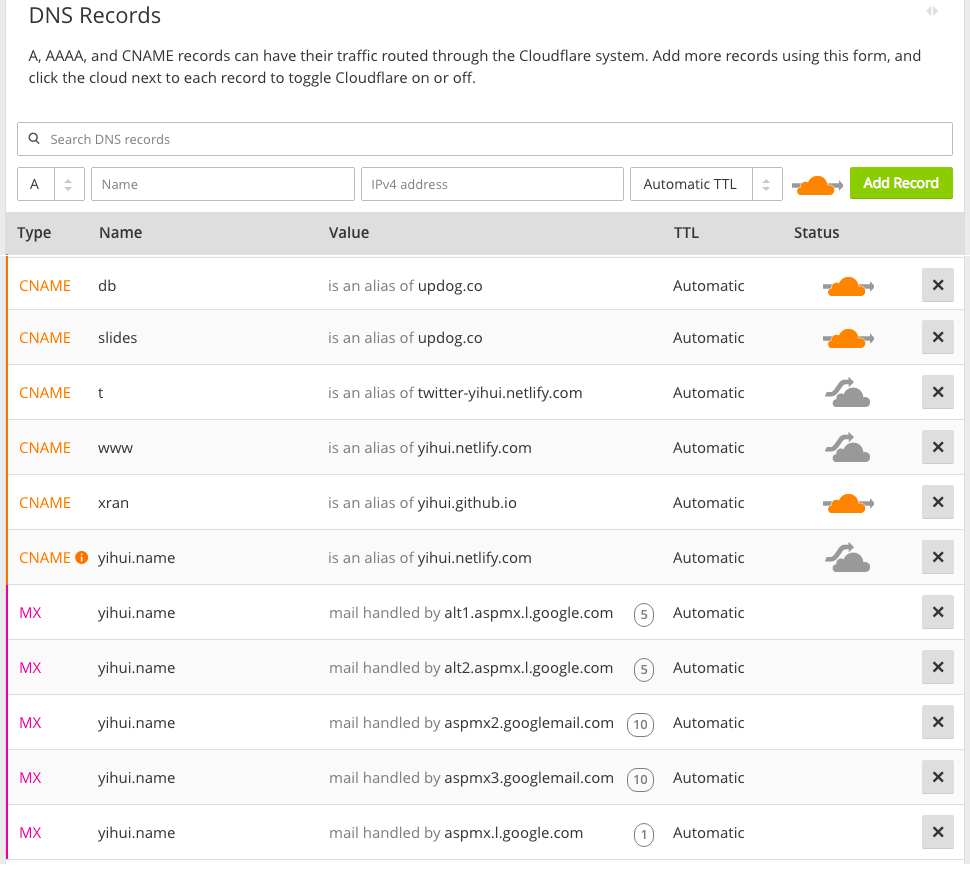
\includegraphics[width=1\linewidth]{images/cloudflare-dns} 

}

\caption{Algunos registros DNS del dominio yihui.name en Cloudflare.}\label{fig:cloudflare-dns}
\end{figure}

Un dominio apex puede tener cualquier cantidad de subdominios. Puede
establecer registros DNS para el dominio apex y cualquier subdominio.
Puede ver en la figura @ref(fig: cloudflare-dns) que tengo varios
subdominios, por ejemplo, \texttt{slides.yihui.name} y
\texttt{xran.yihui.name}.

Como hemos mencionado, un registro A señala un dominio o subdominio a
una dirección IP del servidor host. No utilicé ningún registro A para
mis dominios, ya que todos los servicios que uso, como Updog, GitHub
Pages y Netlify, son compatibles con los registros CNAME. Un registro
CNAME \index{CNAME Record} es un alias que señala un dominio a otro. La
ventaja de utilizar CNAME sobre A es que no tiene que vincular un
dominio a una dirección IP fija. Por ejemplo, el registro CNAME para
\texttt{t.yihui.name} es \texttt{twitter-yihui.netlify.com}. Este último
dominio es proporcionado por Netlify, y no necesito saber dónde alojan
realmente el sitio web. Son libres de mover el host de
\texttt{twitter-yihui.netlify.com}, y no necesitaré actualizar mi
registro de DNS. Cada vez que alguien visita el sitio web
\texttt{t.yihui.name}, el navegador web enrutará el tráfico al dominio
establecido en el registro CNAME. Tenga en cuenta que esto es diferente
de la redirección, es decir, que la URL \texttt{t.yihui.name} no se
redirigirá explícitamente a \texttt{twitter-yihui.netlify.com} (aún se
ve la primera en la barra de direcciones de su navegador).

Normalmente, puede establecer cualquier registro DNS para el dominio
Apex, excepto CNAME, pero configuré un registro CNAME para mi dominio
Apex \texttt{yihui.name}, y esto se debe a que Cloudflare admite el
aplanamiento CNAME. Para obtener más información sobre este tema, puede
leer la publicación
\href{https://www.netlify.com/blog/2017/02/28/to-www-or-not-www\%20/}{``WWW
o no WWW,''} por Netlify. Personalmente, prefiero no usar el subdominio
\texttt{www.yihui.name} para mantener mis URL cortas, así que establezco
un registro CNAME tanto para el dominio principal \texttt{yihui.name}
como para el subdominio \texttt{www}, y Netlify redirigirá
automáticamente el \texttt{www} subdominio al dominio apex. Dicho esto,
si es un principiante, puede ser un poco más fácil configurar y usar el
subdominio \texttt{www}, como lo sugiere Netlify. Tenga en cuenta que
\texttt{www} es un subdominio convencional que suena como un dominio de
apex, pero realmente no lo es; puede seguir esta convención o no como lo
desee.

Para los servicios de correo electrónico, llegué lo suficientemente
temprano \href{https://en.wikipedia.org/wiki/Netizen}{``cibernauta'',} y
cuando registré mi nombre de dominio, Google todavía ofrecía servicios
gratuitos de correo electrónico a propietarios de dominios
personalizados. Así es como puedo tener un buzón personalizado
\texttt{xie@yihui.name}. Ahora tendrá que pagar por
\href{https://gsuite.google.com}{G Suite.} En la figura @ref(fig:
cloudflare-dns) puede ver que he configurado algunos MX (siglas en
inglés de ``intercambio de correo'') registros que apuntan a algunos
servidores de correo de Google. Por supuesto, Google no es la única
opción posible cuando se trata de buzones personalizados.
\href{https://www.migadu.com}{Migadu} dice ser el ``alojamiento de
correo electrónico más asequible''. Puede probar su plan gratuito y ver
si le gusta. A menos que vaya a usar su buzón personalizado
extensivamente y para fines profesionales, el plan gratuito puede ser
suficiente. De hecho, puede crear una dirección de alias en Migadu para
reenviar correos electrónicos a sus otras cuentas de correo electrónico
(como Gmail) si no le importa un buzón personalizado real. Migadu ha
proporcionado instrucciones detalladas sobre cómo establecer los
registros MX para su dominio.

\hypertarget{topicos-avanzados}{%
\chapter{Tópicos avanzados}\label{topicos-avanzados}}

En este apéndice, hablamos de algunos temas avanzados que pueden ser de
interés para desarrolladores y usuarios avanzados.

\hypertarget{mas-opciones-globales}{%
\section{Más opciones globales}\label{mas-opciones-globales}}

Hay algunas opciones globales más avanzadas \index{Opciones globales}
además de las introducidas en la sección @ref(opciones globales), y se
enumeran en la Tabla \ref{tab:global-options2}.

\begin{table}

\caption{\label{tab:global-options2}Unas opciones globales un poco más avanzadas.}
\centering
\begin{tabular}[t]{lll}
\toprule
Option name & Default & Meaning\\
\midrule
blogdown.hugo.dir &  & El directorio ejecutable de Hugo\\
blogdown.method & html & El método de construcción para R Markdown\\
blogdown.publishDir &  & El directorio de publicación para previsualización local\\
blogdown.widgetsID & TRUE & IDs incrementales para HTML widgets?\\
\bottomrule
\end{tabular}
\end{table}

Si desea instalar Hugo en una ruta personalizada, puede establecer la
opción global \texttt{blogdown.hugo.dir} en un directorio para almacenar
el ejecutable Hugo antes de llamar a \texttt{install\_hugo()}, por
ejemplo,
\texttt{options(blogdown.hugo.dir\ =\ \textquotesingle{}\textasciitilde{}/Downloads/hugo\_0.20.1/\textquotesingle{})}.
Esto puede ser útil para que usted use una versión específica de Hugo
para un sitio web específico,\footnote{Puede establecer esta opción por
  proyecto. Consulte la sección @ref(opciones globales) para obtener
  detalles.} O guarde una copia de Hugo en una unidad USB junto con su
sitio web.

La opción \texttt{blogdown.method} se explica en la sección
\ref{métodos}.

Cuando el proyecto de su sitio web está bajo control de versiones en
RStudio IDE, la vista previa continua del sitio puede ser lenta, si
contiene cientos de archivos o más. El directorio de publicación
predeterminado es \texttt{public/} en el directorio raíz del proyecto, y
siempre que realice un cambio en la fuente que desencadena una
reconstrucción, RStudio estará ocupado rastreando los cambios de
archivos en el directorio \texttt{public/}. La demora antes de que vea
el sitio web en RStudio Viewer puede durar 10 segundos o incluso más. Es
por eso que ofrecemos la opción \texttt{blogdown.publishDir}. Puede
establecer un directorio de publicación temporal para generar el sitio
web, y este directorio no debe estar bajo el mismo proyecto de RStudio,
por ejemplo,
\texttt{options\ (blogdown.publishDir\ =\ \textquotesingle{}../public\_site\textquotesingle{})},
lo que significa que el sitio web se generará para el directorio
\texttt{public\_site/} en el directorio padre del proyecto actual.

La opción \texttt{blogdown.widgetsID} solo es relevante si el origen de
su sitio web está bajo control de versiones y tiene widgets HTML en el
sitio web. Si esta opción es \texttt{TRUE} (valor predeteminado), los ID
aleatorios de los HTML widgets se cambiarán a ID incrementales en el
resultado HTML, por lo que es poco probable que estos ID cambien cada
vez que recompile su sitio web; de lo contrario, cada vez obtendrá
diferentes ID aleatorios.

\hypertarget{livereload}{%
\section{LiveReload}\label{livereload}}

Como mencionamos brevemente \index{LiveReload} en la sección
\ref{un-ejemplo-rápido}, puede usar \texttt{blogdown::serve\_site()}
para obtener una vista previa de un sitio web, y la página web se
reconstruirá automáticamente y se volverá a cargar en su navegador web
cuando el archivo fuente se modifica y se guarda. Esto se llama
``LiveReload''.

Hemos proporcionado dos enfoques para LiveReload. El enfoque
predeterminado es a través de \texttt{servr::httw()}, que vigilará
continuamente el directorio del sitio web en busca de cambios de
archivos y reconstruirá el sitio cuando se detecten cambios. Este
enfoque tiene algunos inconvenientes:

\begin{enumerate}
\def\labelenumi{\arabic{enumi}.}
\item
  Es relativamente lento porque el sitio web se regenera por completo
  cada vez. Esto puede no ser un problema real para Hugo, porque Hugo
  suele ser lo suficientemente rápido: se tarda aproximadamente un
  milisegundo en generar una página, por lo que un sitio web con mil
  páginas solo puede tardar aproximadamente un segundo en regenerarse
  por completo.
\item
  El servidor demonizado (vea la sección \ref{opciones-globales} puede
  no funcionar.
\end{enumerate}

Si no está preocupado por los problemas anteriores, le recomendamos que
use el enfoque predeterminado; de lo contrario, puede configurar la
opción global \texttt{options(blogdown.generator.server\ =\ TRUE)} para
usar un enfoque alternativo a LiveReload, que se basa en el soporte
nativo para LiveReload del generador de sitios estáticos. Por el
momento, esto solo se ha probado contra sitios web basados en Hugo. No
funciona con Jekyll y tampoco tuvimos éxito con Hexo.

Este enfoque alternativo requiere la instalación de dos paquetes R
adicionales: \textbf{processx} \citep{R-processx} y \textbf{later}
\citep{R-later}. Puede utilizar este enfoque cuando trabaje
principalmente en publicaciones de Markdown sencillas en lugar de
publicaciones de R Markdown, porque puede ser mucho más rápido obtener
una vista previa de las publicaciones de Markdown utilizando el servidor
web de Hugo. El servidor web puede ser detenido por
\texttt{blogdown::stop\_server()}, y siempre se detendrá cuando la
sesión en R finalice, por lo que puede reiniciar su sesión en R si
\texttt{stop\_server()} no puede detener el servidor por alguna razón.

El servidor web se establece a través del comando \texttt{hugo\ server}
(ver \href{https://gohugo.io/commands/hugo_server/}{su documentación}
para más detalles). Puede pasar argumentos de línea de comandos a través
de la opción global \texttt{blogdown.hugo.server}. El valor
predeterminado para esta opción es
\texttt{c(\textquotesingle{}-D\textquotesingle{},\ \textquotesingle{}-F\textquotesingle{})},
lo que significa mostrar las publicaciones preliminares y futuras en la
vista previa. Queremos resaltar un argumento especial
\texttt{-\/-navigateToChanged} en una versión reciente de Hugo, que le
pide a Hugo que navegue automáticamente a la página modificada. Por
ejemplo, puede establecer las opciones:

\begin{Shaded}
\begin{Highlighting}[]
\KeywordTok{options}\NormalTok{(}\DataTypeTok{blogdown.hugo.server =} \KeywordTok{c}\NormalTok{(}\StringTok{'-D'}\NormalTok{, }\StringTok{'-F'}\NormalTok{, }\StringTok{'--navigateToChanged'}\NormalTok{))}
\end{Highlighting}
\end{Shaded}

Luego, cuando edite un archivo fuente bajo \texttt{content/}, Hugo le
mostrará automáticamente la página de salida correspondiente en el
navegador web.

Tenga en cuenta que Hugo presenta el sitio web desde la memoria de forma
predeterminada, por lo que no se generarán archivos para
\texttt{public/}. Si necesita publicar la carpeta \texttt{public/}
manualmente, deberá compilar manualmente el sitio web a través de
\texttt{blogdown::hugo\_build()} o \texttt{blogdown::build\_site()}.

\hypertarget{local-preview}{%
\section{Construyendo un sitio web para vista previa
local}\label{local-preview}}

La función\index{blogdown::build\_site()}
\texttt{blogdown::build\_site()} tiene un argumento \texttt{local} que
por defecto es \texttt{FALSE}, lo que significa construir el sitio web
para publicación en lugar de vista previa local. El modo
\texttt{local\ =\ TRUE} es principalmente para
\texttt{blogdown::serve\_site()} para presentar el sitio web localmente.
Hay tres diferencias principales entre \texttt{local\ =\ FALSE} y
\texttt{TRUE}. Cuando \texttt{local\ =\ TRUE}:

\begin{itemize}
\item
  La opción \texttt{baseurl} en \texttt{config.toml} se reemplaza
  temporalmente por \texttt{"/"} aunque haya configurado una URL
  completa como \texttt{"http://www.example.com/"}.\footnote{Si su
    \texttt{baseurl} contiene un subdirectorio, será reemplazado por el
    nombre del subdirectorio. Por ejemplo, para
    \texttt{baseurl="\ http://www.example.com/project/\ "},
    \texttt{build\_site(local\ =TRUE)} eliminará temporalmente el nombre
    de dominio y solo usará el valor \texttt{/project/}.} es porque
  cuando un sitio web se va a obtener una vista previa localmente, los
  enlaces deben hacer referencia a los archivos locales. Por ejemplo, se
  debe usar \texttt{/about/index.html} en lugar del enlace
  completo\texttt{http://www.example.com/about/index.html}; la función
  \texttt{serve\_site()} sabe que \texttt{/about/index.html} significa
  el archivo bajo el directorio \texttt{public/}, y puede buscarlo y
  mostrarle el contenido, de lo contrario, su navegador lo llevará al
  sitio web \texttt{http://www.example.com} en lugar de mostrar un
  archivo local.
\item
  Las publicaciones en borrador y futuras siempre se muestran cuando
  \texttt{local\ =\ TRUE}, pero no cuando \texttt{local\ =\ FALSE}. Esto
  es para que pueda obtener una vista previa del borrador y futuras
  publicaciones localmente. Si conoce la
  \href{https://gohugo.io/commands/hugo/}{línea de comandos de Hugo}
  significa que se llama al comando \texttt{hugo} con las banderas
  \texttt{-D\ -F}, o equivalentemente,
  \texttt{-\/-buildDrafts\ -\/-buildFuture}.
\item
  Hay un mecanismo de almacenamiento en caché para acelerar la creación
  de su sitio web: un archivo Rmd no se volverá a compilar cuando su
  archivo de salida \texttt{*.html} sea más reciente (en términos de
  tiempo de modificación de archivos). Si desea forzar
  \texttt{build\_site(local\ =\ TRUE)} para recompilar el archivo Rmd
  incluso si es anterior al resultado HTML, debe eliminar el resultado
  HTML o editar el archivo Rmd para que su hora de modificación sea más
  reciente. Este mecanismo de almacenamiento en caché no se aplica a
  \texttt{local\ =\ FALSE}, es decir,
  \texttt{build\_site(local\ =\ FALSE)}siempre recompilará todos los
  archivos Rmd, porque cuando desee publicar un sitio, es posible que
  deba recompilarlo todo para asegurarse de que el sitio está
  completamente regenerado. Si tiene fragmentos de código que consumen
  mucho tiempo en cualquier archivo Rmd, debe usar cualquiera de estos
  métodos para ahorrar tiempo:

  \begin{itemize}
  \item
    Active el almacenamiento en caché de \textbf{knitr} para la pérdida
    de tiempo de los trozos de código, i.e., la opción de chunk
    \texttt{cache\ =\ TRUE}.
  \item
    No llame \texttt{build\_site()}, sino
    \texttt{blogdown::hugo\_build()} en su lugar
    \index{blogdown::hugo\_build()}. Este último no compila ningún
    archivo Rmd, simplemente ejecuta el comando \texttt{hugo} para
    construir el sitio. Utilice este método solo si está seguro de que
    sus archivos Rmd no necesitan ser recompilados.
  \end{itemize}
\end{itemize}

No necesita preocuparse por estos detalles si su sitio web se genera
automáticamente desde la fuente a través de un servicio como Netlify,
que hará uso de \texttt{baseurl} y no usar \texttt{-D\ -F} de forma
predeterminada. Si publica manualmente la carpeta \texttt{public/}, debe
tener más cuidado:

\begin{itemize}
\item
  Si su sitio web no funciona sin el \texttt{baseurl} completo, o si no
  desea que se publiquen los borradores o las publicaciones futuras, no
  debe publicar el directorio \texttt{public/} generado por
  \texttt{serve\_site()}. Siempre ejecute
  \texttt{blogdown::build\_site()} o \texttt{blogdown::hugo\_build()}
  antes de subir este directorio a un servidor web.
\item
  Si sus borradores y publicaciones futuras contienen información
  (sensible al tiempo), se recomienda mucho eliminar el directorio
  \texttt{/public/} antes de reconstruir el sitio para publicarlo todo
  el tiempo, porque Hugo nunca lo elimina, y su información confidencial
  puede ser presentada por una determinada llamada
  \texttt{build\_site(local\ =\ TRUE)} la última vez y la dejarla en el
  directorio. Si el sitio web es realmente importante, y necesita
  asegurarse de que no se arruinará nada cada vez que lo publique,
  coloque el directorio \texttt{/public/} bajo control de versiones,
  para que pueda ver qué archivos se cambiaron antes de publicar el
  nuevo sitio.
\end{itemize}

\hypertarget{funciones}{%
\section{Funciones del paquete de blogdown}\label{funciones}}

Hay aproximadamente 20 funciones exportadas\index{Funciones} en el
paquete \textbf{blogdown}, y muchas más funciones no exportadas. Las
funciones exportadas están documentadas y puede usarlas después de
\texttt{library(blogdown)} (o mediante \texttt{blogdown\ ::}). Las
funciones no exportadas no están documentadas, pero puede acceder a
ellas a través de \texttt{blogdown:::} (la sintaxis de tres puntos).
Este paquete no es muy complicado y consta de solo 1800 líneas de código
en R (el número viene dado por el comando de conteo de palabras
\texttt{wc}):

Puede consultar el código fuente
(\url{https://github.com/rstudio/blogdown}) si quiere saber más acerca
de una función no exportada. En esta sección, enumeramos de forma
selectiva algunas funciones exportadas y no exportadas en el paquete
para su referencia.

\hypertarget{funciones-exportadas}{%
\subsection{Funciones exportadas}\label{funciones-exportadas}}

Instalación: Puede instalar Hugo con \texttt{install\_hugo()},
actualizar Hugo con \texttt{update\_hugo()}, e instalar un tema de Hugo
con \texttt{install\_theme()}.

Paquetes de comandos de Hugo: \texttt{hugo\_cmd()} es un paquete de
\texttt{system2(\textquotesingle{}hugo\textquotesingle{},\ ...)}, y
todas las funciones posteriores ejecutan comandos específicos de Hugo
basados en esta función de paquete general; \texttt{hugo\_version()}
ejecuta el comando \texttt{hugo\ version} (i.e.,
\texttt{system2(\textquotesingle{}hugo\textquotesingle{},\ \textquotesingle{}version\textquotesingle{})}
en R); \texttt{hugo\_build()} ejecuta \texttt{hugo} con parámetros
opcionales; \texttt{new\_site()} ejecuta \texttt{hugo\ new\ site};
\texttt{new\_content()} ejecuta \texttt{hugo\ new} para crear un nuevo
archivo de contenido, y \texttt{new\_post()} es un paquete basado en
\texttt{new\_content()} para crear una nueva publicación de blog con
metadatos YAML apropiados y nombre de archivo; \texttt{hugo\_convert()}
ejecuta \texttt{hugo\ convert}; \texttt{hugo\_server()} ejecuta
\texttt{hugo\ server}.

Formato de salida: \texttt{html\_page()} es la única función de formato
de salida R Markdown en el paquete. Está heredada desde
\texttt{bookdown::html\_document2()}, que a su vez está heredada de
\texttt{rmarkdown::html\_document()}. Necesita leer la documentación de
estas dos funciones para conocer los posibles argumentos. La sección
\ref{formato-de-salida} tiene información más detallada al respecto.

Funciones de ayuda: \texttt{shortcode()} es una función de ayuda para
escribir abreviatura de Hugo \texttt{\{\{\%\ \%\}\}} en un post Rmd;
\texttt{shortcode\_html()} escribe
\texttt{\{\{\textless{}\ \textgreater{}\}\}}.

Presentar un sitio: \texttt{serve\_site()} inicia un servidor web local
para construir y obtener una vista previa de un sitio de forma continua;
puede detener el servidor a través de \texttt{stop\_server()}, o
reiniciar su sesión en R.

Manejando metadatos YAML: \texttt{find\_yaml()} se puede usar para
encontrar archivos de contenido que contengan un campo YAML especificado
con valores especificados; \texttt{find\_tags()} y
\texttt{find\_categories()} son funciones de contenedor basadas en
\texttt{find\_yaml()} para unir etiquetas y categorías específicas en
archivos de contenido, respectivamente; \texttt{count\_yaml()} se puede
usar para calcular las frecuencias de los campos especificados.

\hypertarget{funciones-no-exportadas}{%
\subsection{Funciones no exportadas}\label{funciones-no-exportadas}}

Algunas funciones no se exportan en este paquete porque es poco probable
que los usuarios promedio las utilicen directamente, y enumeramos un
subconjunto de ellas a continuación:

\begin{itemize}
\item
  Puede encontrar la ruta al ejecutable de Hugo a través de
  \texttt{blogdown:::find\_hugo()}. Si el ejecutable se puede encontrar
  a través de la variable de entorno \texttt{PATH}, simplemente devuelve
  \texttt{\textquotesingle{}hugo\textquotesingle{}}.
\item
  La función auxiliar \texttt{modify\_yaml()} se puede usar para
  modificar los metadatos YAML de un archivo. Tiene un argumento
  \texttt{...} que toma campos YAML arbitrarios, por ejemplo,
  \texttt{blogdown:::modify\_yaml(\textquotesingle{}foo.md\textquotesingle{},\ author\ =\ \textquotesingle{}Frida\ Gomam\textquotesingle{},\ date\ =\ \textquotesingle{}2015-07-23\textquotesingle{})}
  cambiará el campo \texttt{author} en el archivo \texttt{foo.md} a
  \texttt{Frida\ Gomam}, y \texttt{date} a \texttt{2015-07-23}. Hemos
  mostrado el uso avanzado de esta función en la sección
  \ref{Desde-jekyll}.
\item
  También hemos mencionado una serie de funciones para limpiar
  publicaciones de Markdown en la sección \ref{desde-jekyll}. Incluyendo
  \texttt{process\_file()}, \texttt{remove\_extra\_empty\_lines()},
  \texttt{process\_bare\_urls()}, \texttt{normalize\_chars()},
  \texttt{remove\_highlight\_tags()}, y \texttt{fix\_img\_tags()}.
\item
  En la sección @ref(vista previa local), mencionamos un mecanismo de
  almacenamiento en caché basado en el tiempo de modificación del
  archivo. Se implementa en \texttt{blogdown:::require\_rebuild()}, que
  toma dos argumentos de nombres de archivos. El primer archivo es el
  archivo de salida, y el segundo es el archivo de origen. Cuando el
  archivo fuente es anterior al archivo de salida, o el archivo de
  salida no existe o está vacío, esta función devuelve \texttt{TRUE}.
\item
  La función \texttt{blogdown:::Rscript()} es una función de contenedor
  para ejecutar el comando \texttt{Rscript}, que básicamente significa
  ejecutar un script R en una nueva sesión R. Mencionamos esta función
  en el capítulo \ref{otros-generadores}.
\end{itemize}

\hypertarget{rutas-de-figuras-y-otras-dependencias-dep-path}{%
\section{Rutas de figuras y otras dependencias \{\#
dep-path\}}\label{rutas-de-figuras-y-otras-dependencias-dep-path}}

Una de las tareas más desafiantes en el desarrollo del paquete
\textbf{blogdown} es manejar adecuadamente los archivos de dependencia
\index{Archivos de dependencia} de las páginas web. Si todas las páginas
de un sitio web estuvieran en texto plano sin dependencias como imágenes
o librerías de JavaScript, hubiera sido mucho más fácil desarrollar el
paquete \textbf{blogdown}.

Después de que \textbf{blogdown} compila cada documento Rmd en HTML,
intentará detectar las dependencias (si las hay) del código fuente HTML
y las copiará en la carpeta \texttt{static/}, para que Hugo las copie
luego en \texttt{public/} . La detección depende de las rutas de las
dependencias. De forma predeterminada, todas las dependencias, como las
representaciones R y las librerías para HTML widgets, se generan en el
directorio \texttt{foo\_files/} si la Rmd se llama \texttt{foo.Rmd}.
Específicamente, los gráficos R se generan a
\texttt{foo\_files/figure-html/} y el resto de los archivos bajo
\texttt{foo\_files/} son típicamente de HTML widgets.

Los gráficos de R bajo \texttt{content/*/foo\_files/figure-html/} se
copian a \texttt{static/*/foo\_files/figure-html/}, y las rutas en las
etiquetas HTML como
\texttt{\textless{}img\ src="foo\_files/figure-html/bar.png"/\textgreater{}}
se sustituyen por \texttt{/*/foo\_files/figure-html/bar.png}. Tenga en
cuenta que la barra diagonal indica el directorio raíz del sitio web
publicado, y la sustitución funciona porque Hugo copiará
\texttt{*/foo\_files/figure-html/} de \texttt{static/} a
\texttt{public/}.

Cualquier otro archivo bajo \texttt{foo\_files/} se trata como archivo
de dependencia de HTML widgets, y se copiará a
\texttt{static/rmarkdown-libs/}. Las rutas originales en HTML también
serán sustituidos en consecuencia, por ejemplo, del
\texttt{\textless{}script\ src\ =\ "foo\_files/jquery/jquery.min.js"\textgreater{}}
a
\texttt{\textless{}script\ src\ ="/rmarkdown-libs/jquery/jquery.min.js\ "\textgreater{}}.
No importa si estos archivos son generados por HTML widgets o no. Los
enlaces en el sitio web publicado serán correctos y normalmente ocultos
a los lectores de las páginas.\footnote{Por ejemplo, un lector no verá
  la etiqueta \texttt{\textless{}script\textgreater{}} en una página,
  por lo que realmente no importa lo que su atributo \texttt{src} parece
  siempre que sea una ruta que realmente existe.}

No debe modificar la opción \textbf{knitr} chunk \texttt{fig.path} o
\texttt{cache.path} a menos que el proceso anterior sea completamente
claro para usted, y quiera manejar las dependencias usted mismo.

En los casos poco frecuentes en los que \textbf{blogdown} no detecta y
copia algunas de sus dependencias (p.~ej., osó un paquete de HTML
widgets bastante sofisticado que escribe archivos en rutas
personalizadas), tiene dos opciones posibles:

\begin{itemize}
\item
  No ignore \texttt{\_files\$} en la opción \texttt{ignoreFiles} en
  \texttt{config.toml}, no personalice la opción \texttt{permalinks}, y
  configure la opción \texttt{uglyURLs} en \texttt{true}. De esta forma,
  \textbf{blogdown} no sustituirá las rutas que no puede reconocer, y
  Hugo copiará estos archivos a \texttt{public/}. Las ubicaciones de
  archivo relativas del archivo \texttt{*.html} y sus dependencias
  seguirán siendo las mismas cuando se copien en \texttt{public/}, de
  modo que todos los enlaces continuarán funcionando.
\item
  Si elige ignorar \texttt{\_files\$} o ha personalizado la opción
  \texttt{permalinks}, debe asegurarse de que \textbf{blogdown} pueda
  reconocer las dependencias. Un enfoque es usar la ruta devuelta por la
  función auxiliar \texttt{blogdown::dep\_path()} para escribir archivos
  de dependencia adicionales. Básicamente, esta función devuelve la
  opción actual \texttt{fig.path} en \textbf{knitr}, que por defecto es
  \texttt{*\_files/figure-html/}. Por ejemplo, puede generar un trazado
  manualmente bajo \texttt{dep\_path()}, y \textbf{blogdown} lo
  procesará automáticamente (copie el archivo y sustituya la ruta de la
  imagen).
\end{itemize}

Si no entiende todos estos detalles técnicos, le recomendamos que use la
primera opción, y deberá sacrificar los enlaces permanentes
personalizados y las URL limpias (por ejemplo, \texttt{/about.html} en
lugar de \texttt{/about/}). Con esta opción, también puede personalizar
la opción \texttt{fig.path} para fragmentos de código si lo desea.

\hypertarget{html-widgets}{%
\section{HTML widgets}\label{html-widgets}}

No recomendamos utilizar diferentes HTML widgets\index {HTML Widgets} de
muchos paquetes de R en la misma página, ya que es probable que genere
conflictos en JavaScript. Por ejemplo, si su tema utiliza la librería
jQuery, puede entrar en conflicto con la librería jQuery utilizada por
un determinado HTML widget. En este caso, puede cargar de forma
condicional la librería jQuery\index{jQuery} del tema configurando un
parámetro en los metadatos YAML de su publicación y revisando la
plantilla Hugo que carga jQuery. A continuación se muestra el código de
ejemplo para cargar jQuery condicionalmente en una plantilla de Hugo:

\begin{Shaded}
\begin{Highlighting}[]
\NormalTok{\{\{ if not .Params.exclude_jquery\}\}}
\KeywordTok{<script}\OtherTok{ src=}\StringTok{"path/to/jquery.js"}\KeywordTok{></script>}
\NormalTok{\{\{ end \}\}}
\end{Highlighting}
\end{Shaded}

Luego, si configura \texttt{exclude\_jquery:\ true} en los metadatos
YAML de una publicación, la jQuery del tema no se cargará, por lo que no
habrá conflictos cuando los HTML widgets también dependan de jQuery.

Otra solución es el paquete
\href{https://github.com/bhaskarvk/widgetframe}{\textbf{widgetframe}}
\citep{R-widgetframe}. Resuelve este problema incorporando HTML widgets
en
\texttt{\textless{}iframe\textgreater{}\textless{}/iframe\textgreater{}}.
Como un iframe está aislado de la página web principal en la que está
incrustado, no habrá conflictos de JavaScript.

Un widget generalmente no tiene el ancho completo en la página. Para
establecer su ancho al 100\%, puede usar la opción de fragmento de
código \texttt{out.width\ ="100\%"}.

\hypertarget{control-de-versiones}{%
\section{Control de versiones}\label{control-de-versiones}}

Si los archivos fuente de su sitio web están bajo control de versión
\index{Control de versiones}, le recomendamos que agregue al menos estos
dos nombres de carpeta a su archivo \texttt{.gitignore}:

\begin{Shaded}
\begin{Highlighting}[]
\ExtensionTok{blogdown}
\ExtensionTok{public}
\end{Highlighting}
\end{Shaded}

El directorio \texttt{blogdown/} se usa para almacenar archivos de
caché, y es probable que sean inútiles para el sitio web publicado. Solo
\textbf{knitr} puede usarlos, y el sitio web publicado no dependerá de
estos archivos.

El directorio \texttt{public/} debe ignorarse si su sitio web va a ser
(re)incorporado automáticamente en un servidor remoto como Netlify.

Como mencionamos en la sección \ref{dep-path}, las gráficas de R se
copiarán a \texttt{static/}, por lo que puede ver nuevos archivos en GIT
luego de renderizar un archivo Rmd que tenga salida de gráficos. Debe
agregar y confirmar estos nuevos archivos en GIT, ya que el sitio web
los usará.

Aunque no es relevante para \textbf{blogdown}, los usuarios de macOS
deben recordar ignorar \texttt{.DS\_Store} y los usuarios de Windows
deben ignorar \texttt{Thumbs.db}.

Si está relativamente familiarizado con GIT\index{Submódulos de GIT},
hay una técnica especial que puede serle útil para administrar los temas
de Hugo, que se llama ``GIT submodules''. Un submódulo en GIT le permite
administrar una carpeta particular del repositorio principal utilizando
un repositorio remoto diferente. Por ejemplo, si utilizó el
\texttt{hugo-lithium-theme} predeterminado de mi repositorio de GitHub,
es posible que desee sincronizarlo con mi repositorio de vez en cuando,
porque puedo actualizarlo de vez en cuando. Puede agregar el submódulo
GIT a través de la línea de comando:

\begin{Shaded}
\begin{Highlighting}[]
\FunctionTok{git}\NormalTok{ submodule add \textbackslash{}}
\NormalTok{  https://github.com/yihui/hugo-lithium-theme.git \textbackslash{}}
\NormalTok{  themes/hugo-lithium-theme}
\end{Highlighting}
\end{Shaded}

Si existe la carpeta \texttt{themes/hugo-lithium-theme}, debe eliminarla
antes de agregar el submódulo. Luego puede ver una cadena SHA asociada a
la ``carpeta'' \texttt{themes/hugo-lithium-theme} en el estado de GIT de
su repositorio principal que indica la versión del submódulo. Tenga en
cuenta que solo verá la cadena SHA en lugar del contenido completo de la
carpeta. La próxima vez que quiera sincronizarse con mi repositorio,
puede ejecutar el comando:

\begin{Shaded}
\begin{Highlighting}[]
\FunctionTok{git}\NormalTok{ submodule update --recursive --remote}
\end{Highlighting}
\end{Shaded}

En general, si está satisfecho con el aspecto de su sitio web, no
necesita administrar el tema con los submódulos de GIT. Es posible que
las actualizaciones futuras en el repositorio upstream no sean realmente
lo que desea. En ese caso, una copia física y fija del tema es más
apropiada para usted.

\hypertarget{default-plantilla}{%
\section{La plantilla por defecto en HTML}\label{default-plantilla}}

Como mencionamos en la sección \ref{formato-de-salida}, el formato de
salida predeterminado para un documento Rmd en \textbf{blogdown} es
\texttt{blogdown::html\_page}. Este formato transfiere una plantilla
HTML mínima a Pandoc\index{Pandoc} de manera predeterminada:

\begin{Shaded}
\begin{Highlighting}[]
\NormalTok{$for(header-includes)$}
\NormalTok{$header-includes$}
\NormalTok{$endfor$}
\NormalTok{$if(highlighting-css)$}
\KeywordTok{<style}\OtherTok{ type=}\StringTok{"text/css"}\KeywordTok{>}
\NormalTok{$highlighting-css$}
\KeywordTok{</style>}
\NormalTok{$endif$}
\NormalTok{$for(css)$}
  \KeywordTok{<link}\OtherTok{ rel=}\StringTok{"stylesheet"}\OtherTok{ href=}\StringTok{"$css$"}\OtherTok{ type=}\StringTok{"text/css"} \KeywordTok{/>}
\NormalTok{$endfor$}

\NormalTok{$for(include-before)$}
\NormalTok{$include-before$}
\NormalTok{$endfor$}
\NormalTok{$if(toc)$}
\KeywordTok{<div}\OtherTok{ id=}\StringTok{"$idprefix$TOC"}\KeywordTok{>}
\NormalTok{$toc$}
\KeywordTok{</div>}
\NormalTok{$endif$}

\NormalTok{$body$}

\NormalTok{$for(include-after)$}
\NormalTok{$include-after$}
\NormalTok{$endfor$}
\end{Highlighting}
\end{Shaded}

Puede encontrar este archivo de plantilla a través de
\texttt{blogdown:::pkg\_file(\textquotesingle{}resources\textquotesingle{},\ \textquotesingle{}template-minimal.html\textquotesingle{})}
en R, y esta ruta de archivo es el valor predeterminado del argumento
\texttt{template} de \texttt{html\_page()}. Puede cambiar esta plantilla
predeterminada, pero debe entender qué se supone que debe hacer esta
plantilla primero.

Si está familiarizado con las plantillas de Pandoc, debe tener en cuenta
que esta no es una plantilla HTML completa, por ejemplo, no tiene las
etiquetas \texttt{\textless{}html\textgreater{}},
\texttt{\textless{}head\textgreater{}}, o
\texttt{\textless{}body\textgreater{}}. Eso es porque no necesitamos ni
queremos que Pandoc nos devuelva un documento HTML completo. Lo
principal que queremos que Pandoc haga es convertir nuestro documento
Markdown a HTML, y darnos el cuerpo del documento HTML, que está en la
variable de plantilla \texttt{\$body\$}. Una vez que tengamos el cuerpo,
podemos pasarlo a Hugo, y Hugo usará su propia plantilla para incrustar
el cuerpo y generar el documento HTML completo. Vamos a explicar esto
con un ejemplo mínimo. Supongamos que tenemos un documento R Markdown
\texttt{foo.Rmd}:

\begin{Shaded}
\begin{Highlighting}[]
\NormalTok{---}
\NormalTok{title: "Hola mundo"}
\NormalTok{author: "Yihui Xie"}
\NormalTok{---}

\NormalTok{Encontré un paquete llamado **blogdown**.}
\end{Highlighting}
\end{Shaded}

Primero se convierte a un archivo HTML \texttt{foo.html} a través de
\texttt{html\_page()}, y tenga en cuenta que los metadatos YAML se
ignoran por ahora:

\begin{Shaded}
\begin{Highlighting}[]
\NormalTok{Encontré un paquete llamado }\KeywordTok{<strong>}\NormalTok{blogdown}\KeywordTok{</strong>}\NormalTok{.}
\end{Highlighting}
\end{Shaded}

Luego \textbf{blogdown} leerá los metadatos YAML del archivo fuente Rmd
e insertará los metadatos en el archivo HTML para que se convierta en:

\begin{Shaded}
\begin{Highlighting}[]
\NormalTok{---}
\NormalTok{title: "Hola mundo"}
\NormalTok{author: "Yihui Xie"}
\NormalTok{---}

\NormalTok{Encontré un paquete llamado }\KeywordTok{<strong>}\NormalTok{blogdown}\KeywordTok{</strong>}\NormalTok{.}
\end{Highlighting}
\end{Shaded}

Este es el archivo que Hugo debe recoger y eventualmente convertir a una
página HTML de un sitio web. Como Pandoc procesó el cuerpo de Markdown
para HTML, Hugo básicamente usará el HTML. Así es como eludimos el motor
Markdown BlackFriday de Hugo.

Además de \texttt{\$body\$}, puede haber notado otras variables de
plantilla de Pandoc como \texttt{\$header-includes\$}, \texttt{\$css\$},
\texttt{\$include-before\$}, \texttt{\$toc\$}, y
\texttt{\$include-after\$}. Estas variables permiten personalizar el
formato \texttt{html\_page}. Por ejemplo, si desea generar una tabla de
contenido y aplicar una hoja de estilo CSS adicional a una página
determinada, puede establecer \texttt{toc} en \texttt{true} y pasar la
ruta de la hoja de estilo al argumento \texttt{css} de
\texttt{html\_page()}, por ejemplo,

\begin{Shaded}
\begin{Highlighting}[]
\OtherTok{---}
\FunctionTok{title:}\AttributeTok{ }\StringTok{"Hola mundo"}
\FunctionTok{author:}\AttributeTok{ }\StringTok{"Yihui Xie"}
\FunctionTok{output:}
  \FunctionTok{blogdown:}\AttributeTok{:html_page:}
    \FunctionTok{toc:}\AttributeTok{ true}
    \FunctionTok{css:}\AttributeTok{ }\StringTok{"/css/my-style.css"}
\OtherTok{---}
\end{Highlighting}
\end{Shaded}

\hypertarget{muxe9todos}{%
\section{Diferentes métodos de construcción}\label{muxe9todos}}

Si su sitio web no contiene ningún archivo Rmd, es muy sencillo
presentarlo, solo una llamada al sistema al comando \texttt{hugo}.
Cuando su sitio web contiene archivos Rmd, \textbf{blogdown} ha
proporcionado dos métodos de representación para compilar estos archivos
Rmd. Se puede construir un sitio web usando la función
\texttt{blogdown::build\_site()}:

\begin{Shaded}
\begin{Highlighting}[]
\KeywordTok{build_site}\NormalTok{(}\DataTypeTok{local =} \OtherTok{FALSE}\NormalTok{, }\DataTypeTok{method =} \KeywordTok{c}\NormalTok{(}\StringTok{"html"}\NormalTok{, }\StringTok{"custom"}\NormalTok{),}
  \DataTypeTok{run_hugo =} \OtherTok{TRUE}\NormalTok{)}
\end{Highlighting}
\end{Shaded}

Como se menciona en la sección \ref{opciones-globales}, el valor
predeterminado del argumento \texttt{método} está determinado por la
opción global \texttt{blogdown.method}, y puede establecer esta opción
en \texttt{.Rprofile}.

Para
\texttt{method\ =\ \textquotesingle{}html\textquotesingle{}},\texttt{build\_site()}
renderiza \texttt{*.Rmd} a \texttt{*.html}, y \texttt{*.Rmarkdown} a
\texttt{*.markdown}, y mantiene los \texttt{*.html}/\texttt{*.markdown}
archivos de salida bajo el mismo directorio que los archivos
\texttt{*.Rmd}/\texttt{*.Rmarkdown}.

Un archivo Rmd puede generar dos directorios para figuras
(\texttt{*\_files/}) y caché (\texttt{*\_caché/}), respectivamente, si
tiene salida de gráficos o HTML widgets \citep{R-htmlwidgets} en los
fragmentos de código R, o habilitada la opción de fragmento
\texttt{cache\ =\ TRUE} para el almacenamiento en caché. En el
directorio de figuras, habrá un subdirectorio \texttt{figure-html/} que
contiene los archivos de salida de trazado, y posiblemente otros
subdirectorios que contengan dependencias HTML de widgets HTML (por
ejemplo, \texttt{jquery/}). El directorio de figuras se mueve a
\texttt{/static/}, y el directorio de caché se mueve a
\texttt{/blogdown/}.

Después de ejecutar \texttt{build\_site()}, su sitio web está listo para
ser compilado por Hugo. Esto le da la libertad de usar servicios de
implementación como Netlify (capítulo \ref{implementación}), donde ni R
ni \textbf{blogdown} están disponibles, pero Hugo sí lo está.

Para \texttt{method\ =\ \textquotesingle{}custom\textquotesingle{}},
\texttt{build\_site()} no procesará ningún archivo R Markdown ni llamará
a Hugo para construir el sitio. No importa qué método elija usar,
\texttt{build\_site()} siempre buscará un script en R
\texttt{/R/build.R} y lo ejecutará si existe. Esto le da total libertad
para hacer lo que quiera para el sitio web. Por ejemplo, puede llamar a
\texttt{knitr::knit()} para compilar Rmd a Markdown (\texttt{*.md}) en
este script de R en lugar de usar \texttt{rmarkdown::render()}. Esta
característica está diseñada para usuarios avanzados que están realmente
familiarizados con el paquete \textbf{knitr}\footnote{Honestamente,
  originalmente fue diseñado para que el propio Yihui construya su
  propio sitio web, pero se dio cuenta de que esta característica podría
  liberar a los usuarios de Hugo. Por ejemplo, es posible usar Jekyll
  (otro popular generador de sitios estáticos) con \textbf{blogdown},
  también.} Y Hugo u otros generadores de sitios web estáticos (ver
capítulo \ref{otros-generadores}).

Cuando \texttt{R/build.R} existe y
\texttt{method\ =\ \textquotesingle{}html\textquotesingle{}}, los
archivos R Markdown se tejen primero, luego se ejecuta el script
\texttt{R/build.R}, y finalmente se llama a Hugo para construir el sitio
web.

\hypertarget{experiencia-personal}{%
\chapter{Experiencia personal}\label{experiencia-personal}}

Empecé a bloguear en blogchina.com en 2005, me mudé a blog.com.cn, luego
a MSN Space, y finalmente compré mi propio dominio \texttt{yihui.name} y
un host virtual. Primero usé una aplicación PHP llamada Bo-Blog, luego
cambié a WordPress, y luego a Jekyll. Finalmente me mudé a Hugo. Aunque
me he mudado varias veces, todas mis publicaciones se han conservado, y
todavía se puede ver mi primera publicación en chino en 2005. A menudo
hago mi mejor esfuerzo para no introducir enlaces rotos (que conducen a
la página 404) cada vez que cambio la publicación backend de mi sitio
web. Cuando sea demasiado difícil preservar los enlaces originales de
ciertas páginas, redirigiré las URL rotas a las nuevas URL. Es por eso
que es importante que su sistema admita redirecciones, y en particular,
301 redirecciones (Netlify hace un buen trabajo aquí). Estas son algunas
de mis reglas de redireccionamiento:
\url{https://github.com/rbind/yihui/blob/master/static/_redirects}. Por
ejemplo, \texttt{http://yihui.name/en/feed/} era la fuente RSS de mis
viejos blogs de WordPress y Jekyll en inglés, y Hugo genera la fuente
RSS a \texttt{/en/index.xml} en su lugar, así que necesita redirigir
\texttt{/en/feed/} a \texttt{/en/index.xml}.

Google ha proporcionado varias herramientas para ayudarlo a obtener más
información sobre su sitio web. Por ejemplo,
\href{https://analytics.google.com}{Google Analytics} puede recopilar
estadísticas de visitantes y dar sugerencias de velocidad para su sitio
web. \href{https://www.google.com/webmasters/}{Google Webmasters} puede
mostrarle los enlaces rotos que encuentra. Uso estas herramientas con
frecuencia.

Creo firmemente en el valor de escribir. Con los años, he escrito más de
1000 publicaciones en chino e inglés. Algunos son largos, y la mayoría
son cortos. El tamaño total de estos archivos de texto es de
aproximadamente 5 Mb. En retrospectiva, la mayoría de los mensajes
probablemente no son valiosos para los lectores en general (algunos son
pensamientos aleatorios, y algunos son mis discursos), pero creo que me
beneficié mucho de escribir en dos aspectos:

\begin{enumerate}
\def\labelenumi{\arabic{enumi}.}
\item
  Si me siento y me concentro en escribir un tema pequeño por un tiempo,
  a menudo siento que mis pensamientos serán más claros. Una gran
  diferencia entre escribir y hablar es que siempre puedes reorganizar
  las cosas y revisarlas al escribir. No creo que escribir en redes
  sociales cuente. 140 caracteres bien pueden ser reflexivos, pero
  siento que hay mucho caos allí. Es difícil plantear pensamientos
  sistemáticos solo a través de mensajes cortos, y estos mensajes
  rápidos a menudo se olvidan rápidamente.
\item
  Sé que algunos bloggers están en contra de los comentarios, por lo que
  no abren comentarios al público. Todavía no he tenido una experiencia
  muy negativa con los comentarios. Por el contrario, constantemente
  encuentro inspiraciones de los comentarios. Por ejemplo,
  \href{https://yihui.name/en/2013/04/travis-ci-for-r/}{Estaba pensando}
  si era posible verificar automáticamente los paquetes en R en la nube
  a través de Travis CI. En ese momento (abril de 2013), creo que no
  mucha gente en la comunidad R había comenzado a usar Travis CI, aunque
  no estoy seguro si fui la primera persona que experimentó con esta
  idea. Sentí que Travis CI podría ser prometedor, pero no fue
  compatible con R en ese momento. Alguien llamado Vincent Arel-Bundock
  (todavía no lo conozco) me contó un truco en un comentario, que de
  repente me iluminó y rápidamente descubrí una solución. En octubre de
  2013, Craig Citro comenzó un trabajo más sólido en el apoyo de R en
  Travis CI. No sé si vio mi publicación en el blog. De todos modos,
  creo que Travis CI ha tenido un impacto sustancial en los
  desarrolladores de paquetes en R, que es algo grandioso para la
  comunidad de R.
\end{enumerate}

Otro beneficio relativamente pequeño es que a menudo voy a mis propios
posts para aprender algunas cosas técnicas que he olvidado. Por ejemplo,
me resulta difícil recordar la sintaxis de diferentes tipos de
aserciones de ancho cero en expresiones regulares similares a Perl:
\texttt{(?=...)}, \texttt{(?!...)}, \texttt{(?\textless{}=...)},
y\texttt{(?\textless{}!...)}. Así que escribí una breve publicación en
el blog y me di algunos ejemplos mínimos. Después de volver a esa
publicación varias veces, finalmente puedo recordar cómo usar estas
expresiones regulares.

\bibliography{book.bib,packages.bib}

\backmatter
\printindex

\end{document}
